\chapter{Battery Emulator Setup}
% \stepcounter{chapter}\addcontentsline{toc}{chapter}{Simulink Modeling and Verification}

\section{Introduction}
The block specifications obtained from the Simulink model is considered as a starting point for the circuit level design in the Cadence. The core part of the architecture of the Extended-Range ADC to be implemented, as shown in Fig. \ref{fig:prop_eradc_circ}, consists of two integrators, 3-bit quantizer, 3-bit DAC and Inter-Stage Gain block. While the supporting-blocks required for the complete implementation are the biasing for the op-amps in the two integrators and the ISG, timing block to generate clock phases and some control signals, the Dynamic Element Matching (DEM) block for the suppression of the harmonics due to DAC unit element mismatch and the Wallace tree encoder to convert the thermometer code to binary code which is read outside for the post-processing.

%
\begin{table}[h]
\centering
\begin{tabular}{c|c|c|c}
\Xhline{4\arrayrulewidth}
\textbf{Sr. No.} & \textbf{Parameter} & \textbf{First Op-Amp} & \textbf{Second Op-Amp} \\ \hline
1 & Gain (dB) & 50 & 50 \\ \hline 
2 & GBW (MHz) & 190 & 160 \\ \hline
3 & Slew Rate (V/µs) & 190 & 160 \\ \hline
4 & Voltage Swing (V) & 0.3 & 1.2 \\ \Xhline{4\arrayrulewidth}
\end{tabular}
\caption{Op-Amp specification requirements}
\label{tab:opamp_specs}
\end{table}
%
It can be observed from Fig. \ref{SNR_G1} and Fig. \ref{SNR_G2}, though the low frequency gain requirement for the case $N_{SD}=3$ and $N_{RS}=5$ to achieve maximum SNR of 86~dB is around 80~dB, there is no significant degradation in SNR, if gain drops down to 50~dB. This relaxation in the gain requirement then helps to achieve the GBW value. The Table.\ref{tab:opamp_specs} shows the first and the second op-amp requirements for given specifications for the ADC architecture.
% \begin{table}[h]
% \centering
% \begin{tabular}{c|c|c|c}
% \hline \xrowht{15pt}
% \textbf{Sr. No.} & \textbf{Parameter} & \textbf{First Op-Amp} & \textbf{Second Op-Amp} \\ \hline\xrowht{10pt}
% 1 & Gain ($dB$) & 60 & 60 \\ \xrowht{10pt}
% 2 & GBW ($MHz$) & 250 & 140 \\ \xrowht{10pt}
% 3 & Slew Rate ($V/\mu s$) & 250 & 120 \\ \xrowht{10pt}
% 4 & Voltage Swing ($V$) & 0.3 & 1.2 \\ \hline
% \end{tabular}
% \end{table}
\section{Integrators}
%
\begin{figure}[ht]
\centering
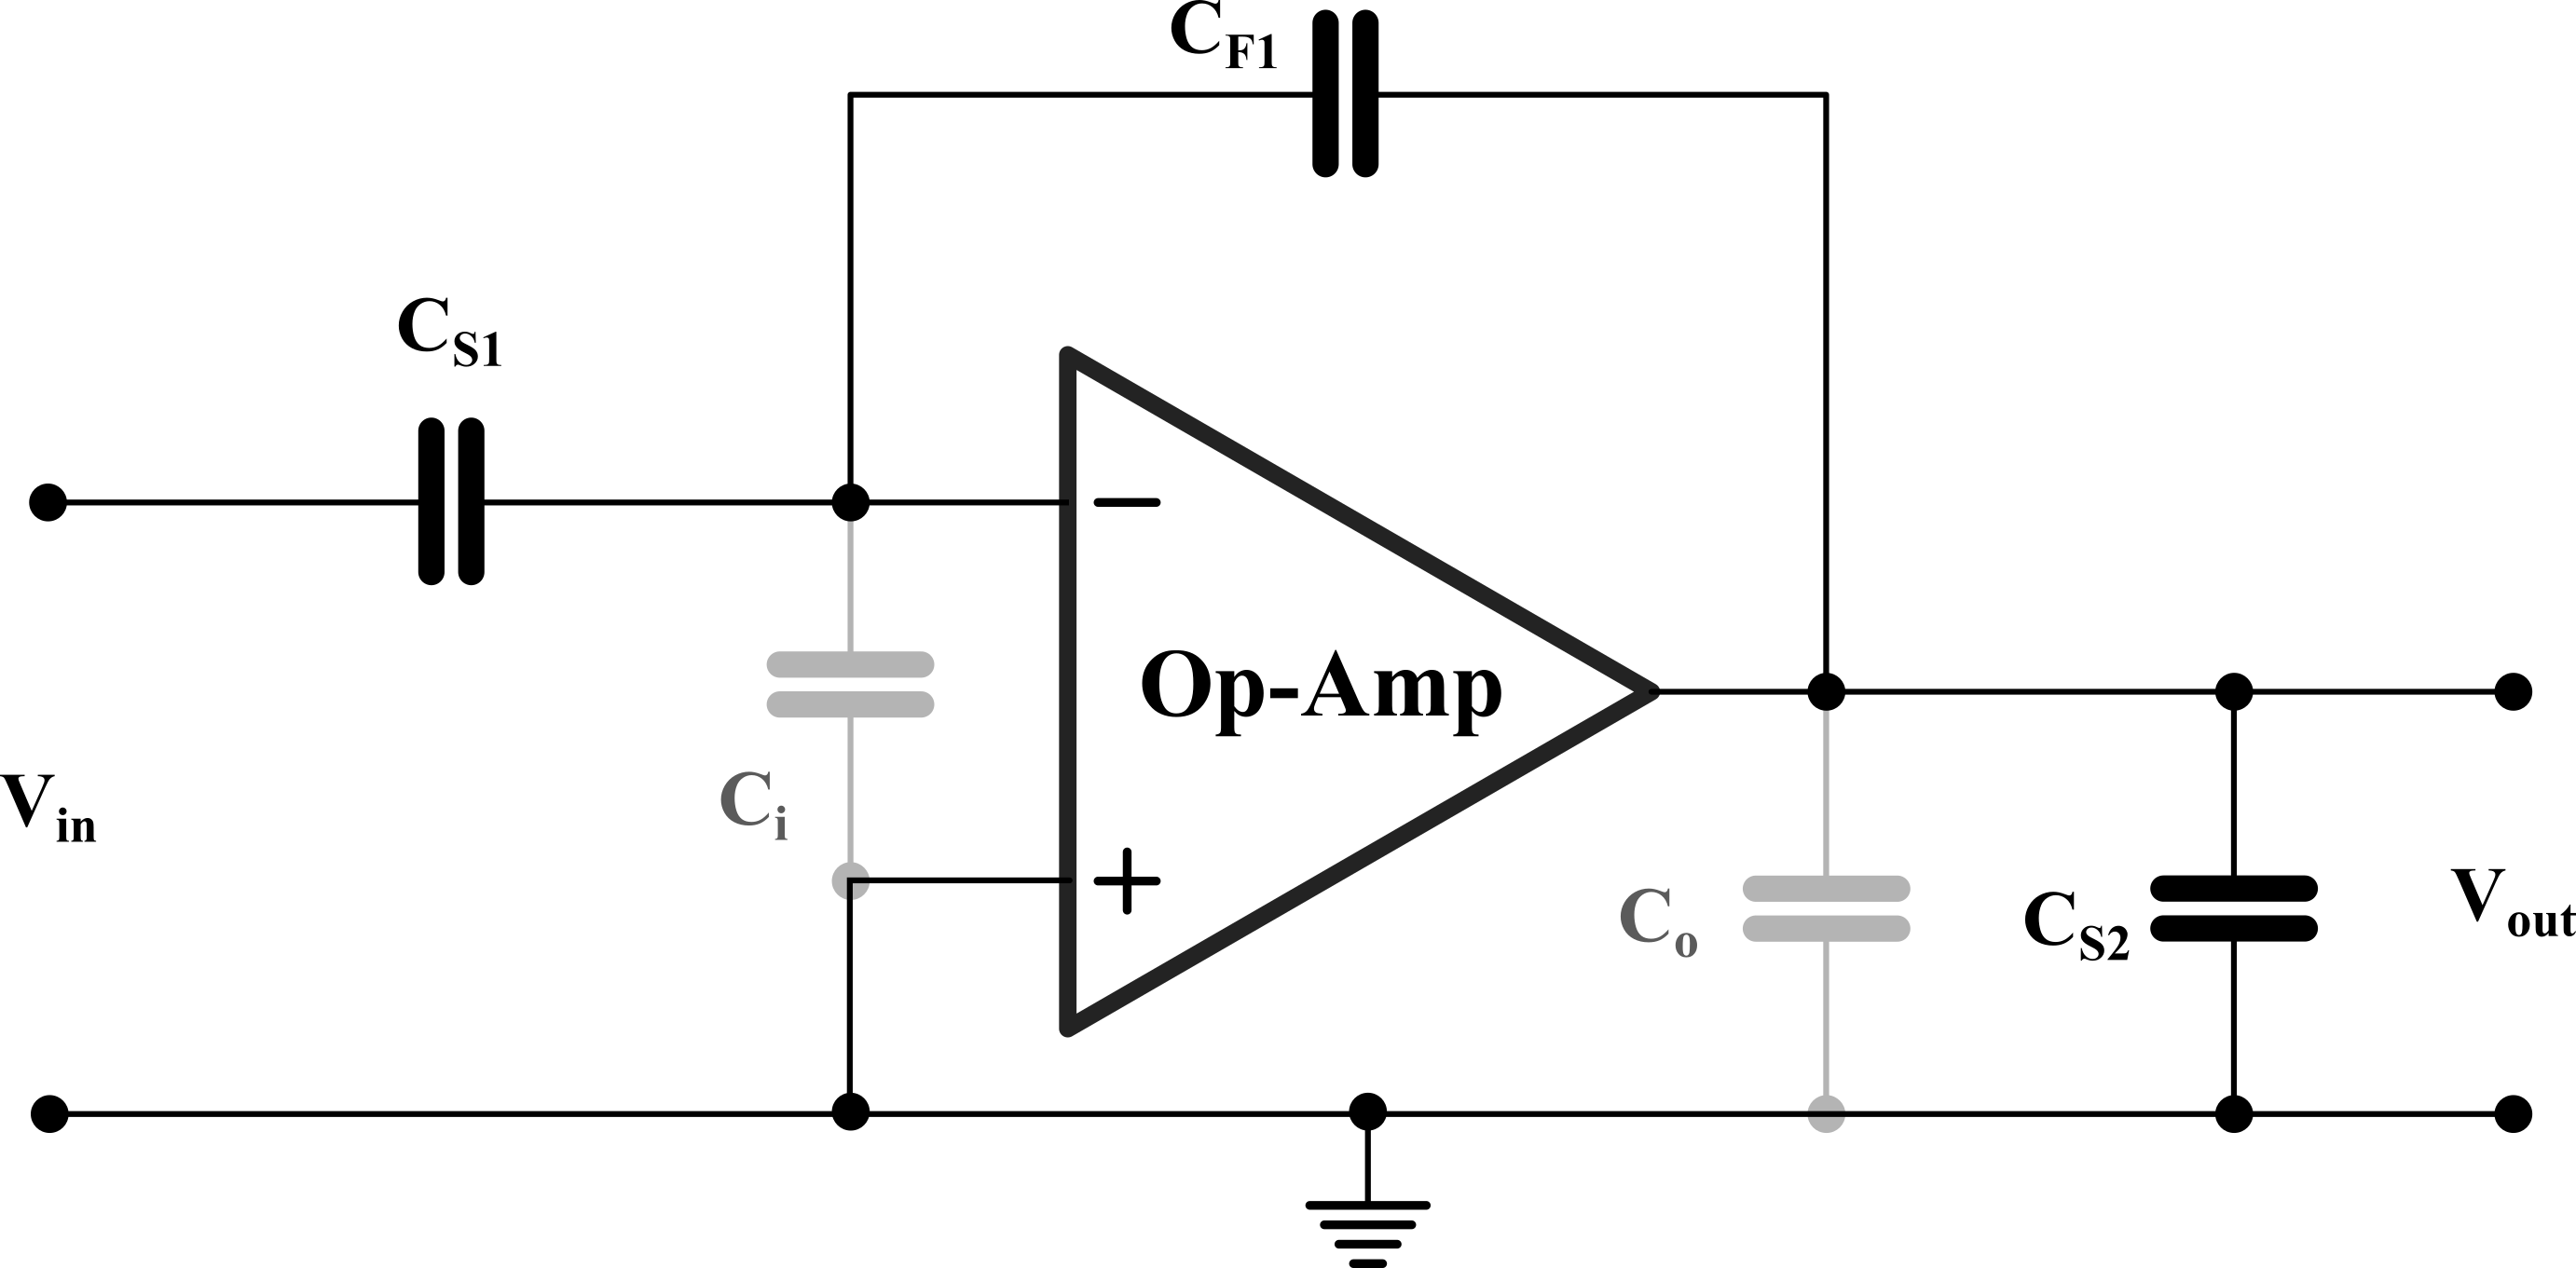
\includegraphics[width=0.6\columnwidth]{Chap05/Figures/integrator.png}
\caption{Single Ended representation of the First Integrator in the integrating phase}
\label{INT1_INTPHS}
\end{figure}
%
The choice of the architecture of the op-amps has various design constraints like power consumption, gain, GBW and slew rate, load capacitance, voltage swing etc. Two-stage op-amp is usually preferred when the gain high requirement has to be fulfilled and the power consumption is not of the concern. It also achieves high output voltage swing since at the output stage, there are just two transistors in stack. However, if along with gain the power consumption and GBW are also important, the solution could be the telescopic amplifier. Nevertheless, stack of 5 transistors between the rails in the telescopic structure limits the swing at the output. But considering the requirement, it is a good option for the op-amp in the first integrator. Swing of the signal at the output of second integrator is considerably high. Therefore, the op-amp structure or the constraints for the second integrator can be reconsidered if similar op-amp architecture has to be reused.

\subsection{Op-Amp for the First Integrator:}
In the integrating phase of the circuit of the first integrator appears like one shown in Fig. \ref{INT1_INTPHS} where $C_{S1}$ is the sampling capacitor, $C_{F1}$ is the feedback capacitor of first integrator, $C_{i}$ is the parasitic capacitor at the virtual ground node, $C_{o}$ is the parasitic capacitor at the output node of the op-amp and $C_{S2}$ is the sampling capacitor of the second integrator. The value of the sampling capacitor $C_{S1}$ is $400\ fF$, therefore the value of the feedback capacitor is also kept $400\ fF$ for the purpose to keep coefficient of the integrator to 1. 
%
\begin{figure}[h]
\centering
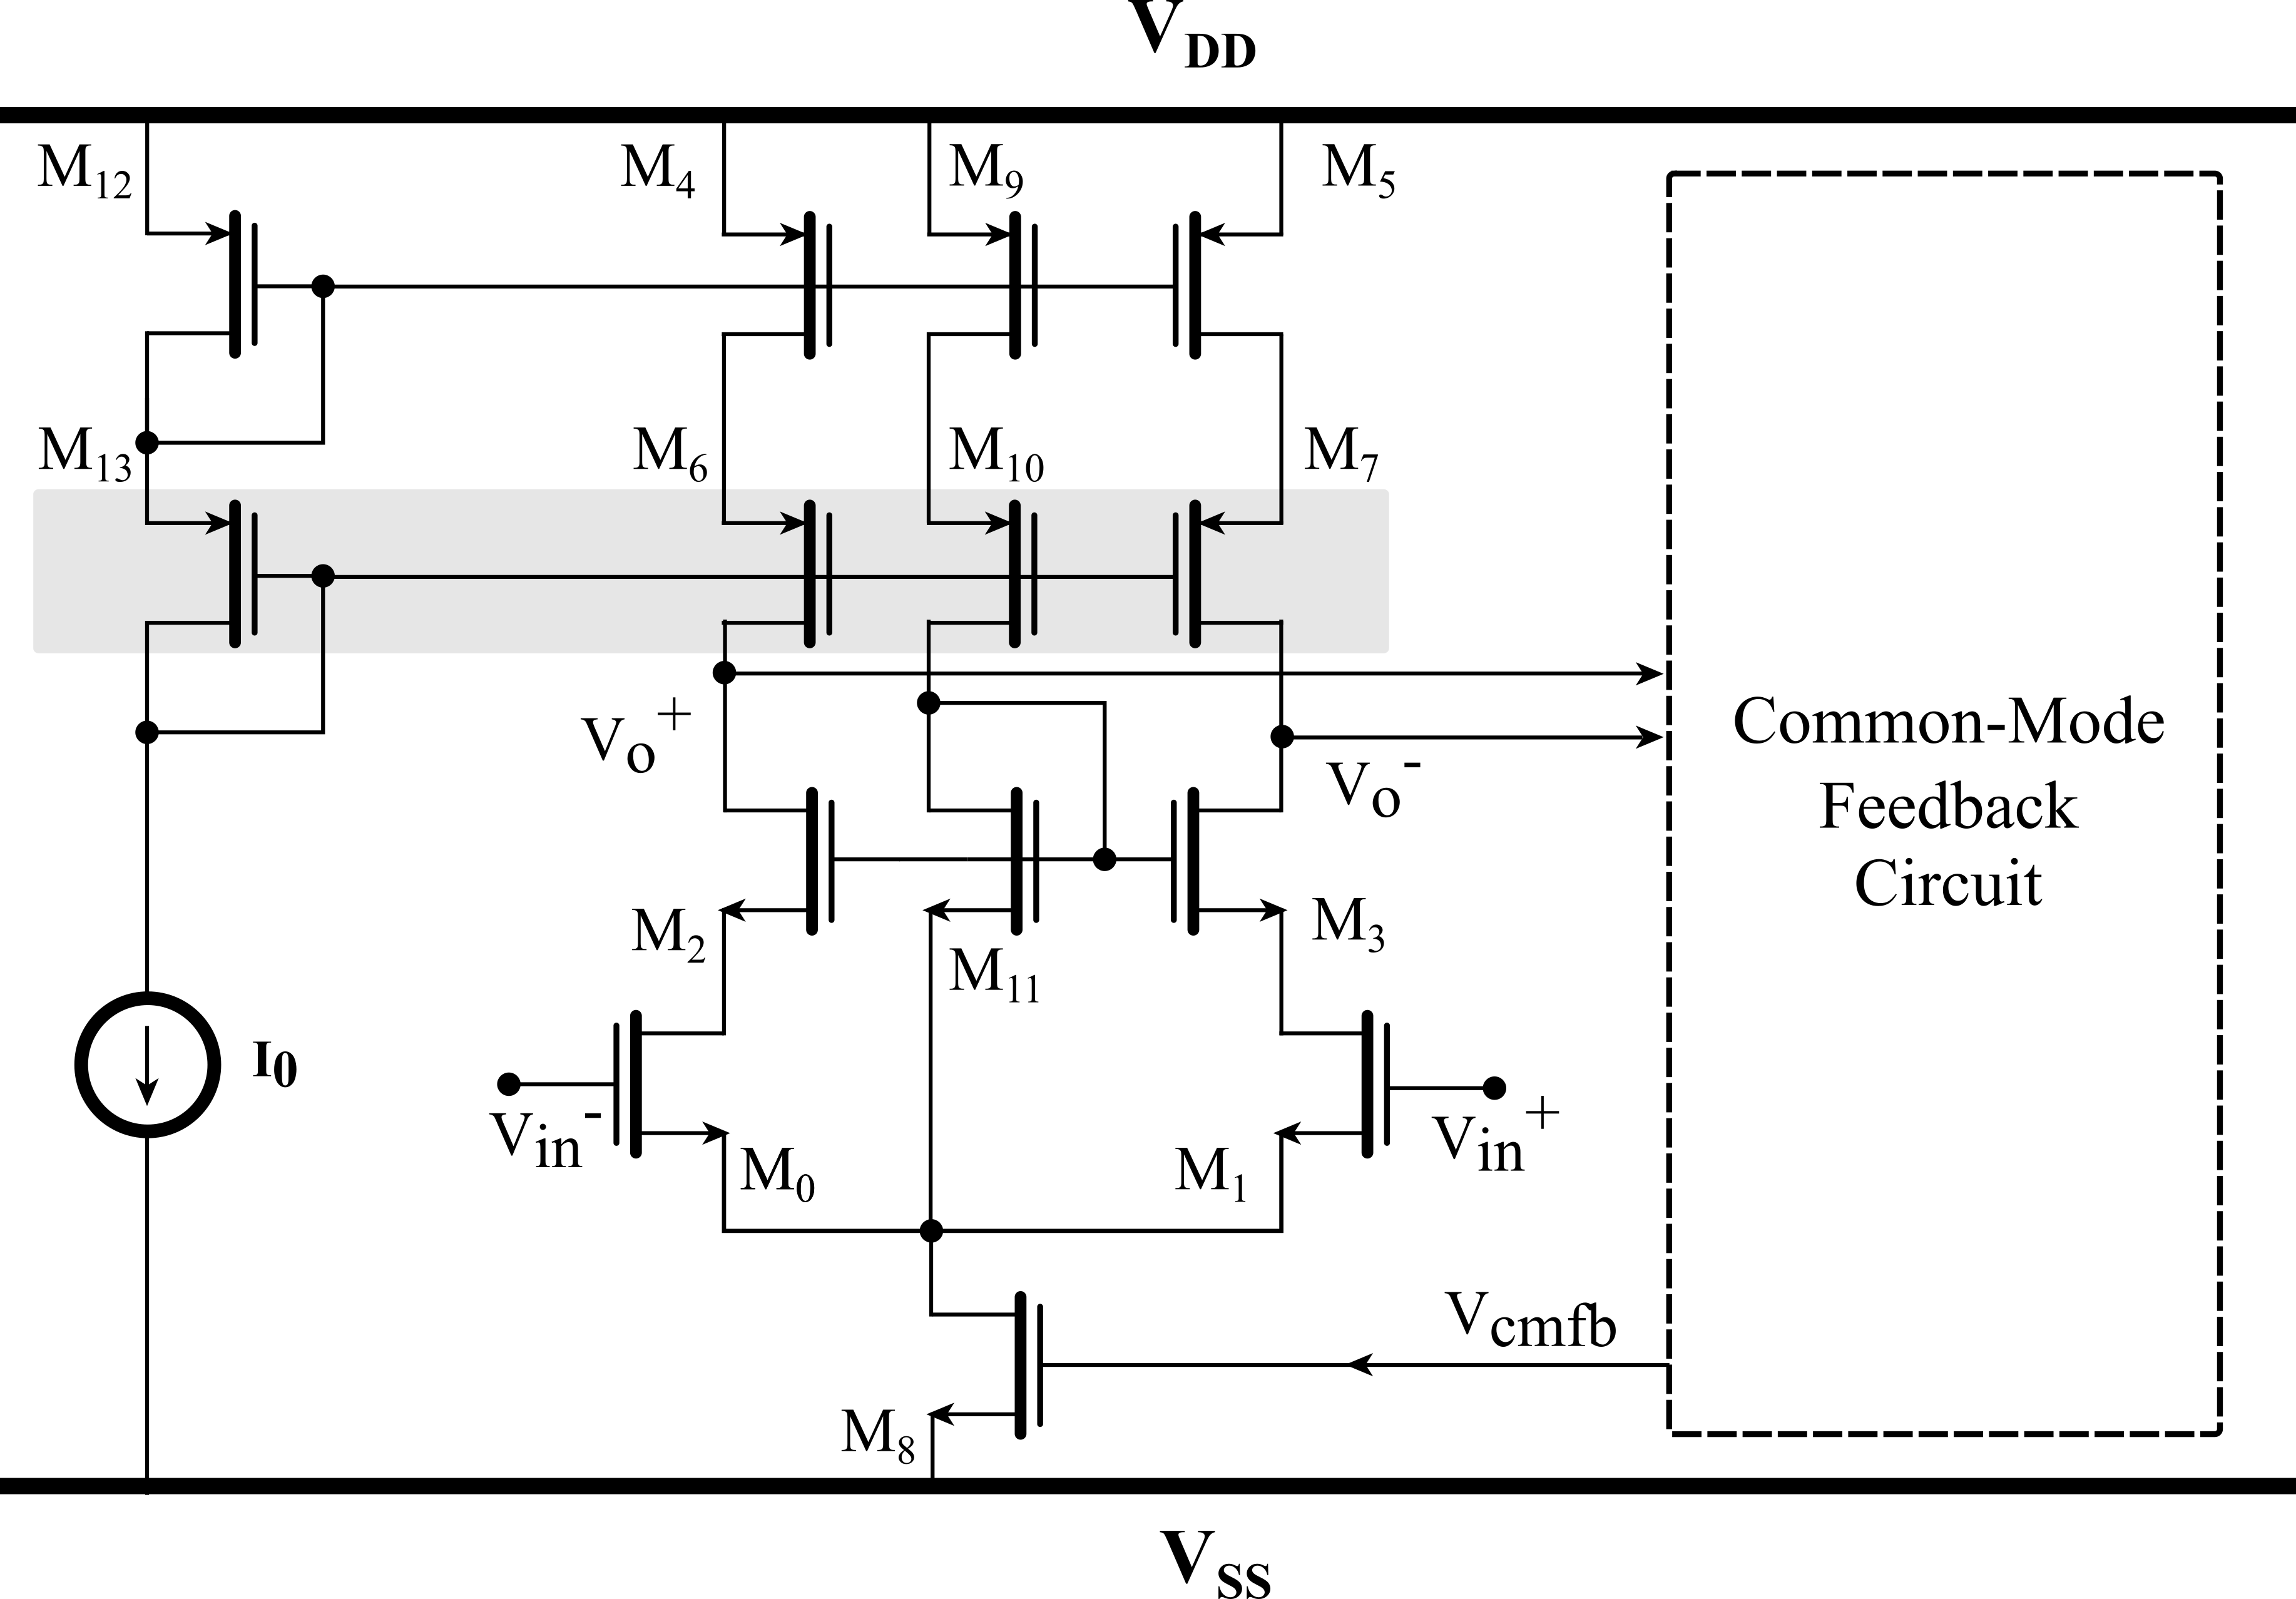
\includegraphics[width=0.85\columnwidth]{Chap05/Figures/telescopic.png}
\caption{Conventional Telescopic Amplifier Circuit Diagram}
\label{fig:TELE_AMP}
\end{figure}
%

% Similarly the value of sampling cap of the second integrator is also kept $400\ fF$, while that for $C_{i}$ and $C_{o}$ are assumed to be $100\ fF$ (assumption, prior to the design). 
From the setup in Fig. \ref{INT1_INTPHS}, the load capacitance $C_L$ and the feedback factor $\beta$, for the first integrator, can be estimated as,
\begin{equation}
    C_{L1}=\frac{C_{F1}\left(C_{S1}+C_{i}\right)}{C_{F1}+C_{S1}+C_{i}}+C_{o}+C_{S2}
    \label{CL1}
\end{equation}
\begin{equation}
    \beta_{1}=\frac{C_{F1}}{C_{F1}+C_{S1}+C_{i}}
    \label{BETA1}
\end{equation}

Making the use of the equations above, the load capacitance and the feedback factor turns out to be around $725\ fF$ and 0.44 respectively. Consequently, the design of the first op-amp has to be done to ensure the loop gain of $60\ dB$, loop GBW of $190\ MHz$, SR of $190\ V/\mu s$ and voltage swing of $300\ mV$ for the load of $725\ fF$ and $\beta$ of 0.44. 
%
\begin{equation}
    Loop\ GBW = \beta_1 \ GBW_{OL} = \beta_1 \frac{g_m}{2\pi C_{L1}}
\end{equation}
%
%
\begin{equation}
    Loop\ Gain = \beta_1\ A_{OL}
\end{equation}
%
%
\begin{figure}[h]
\centering
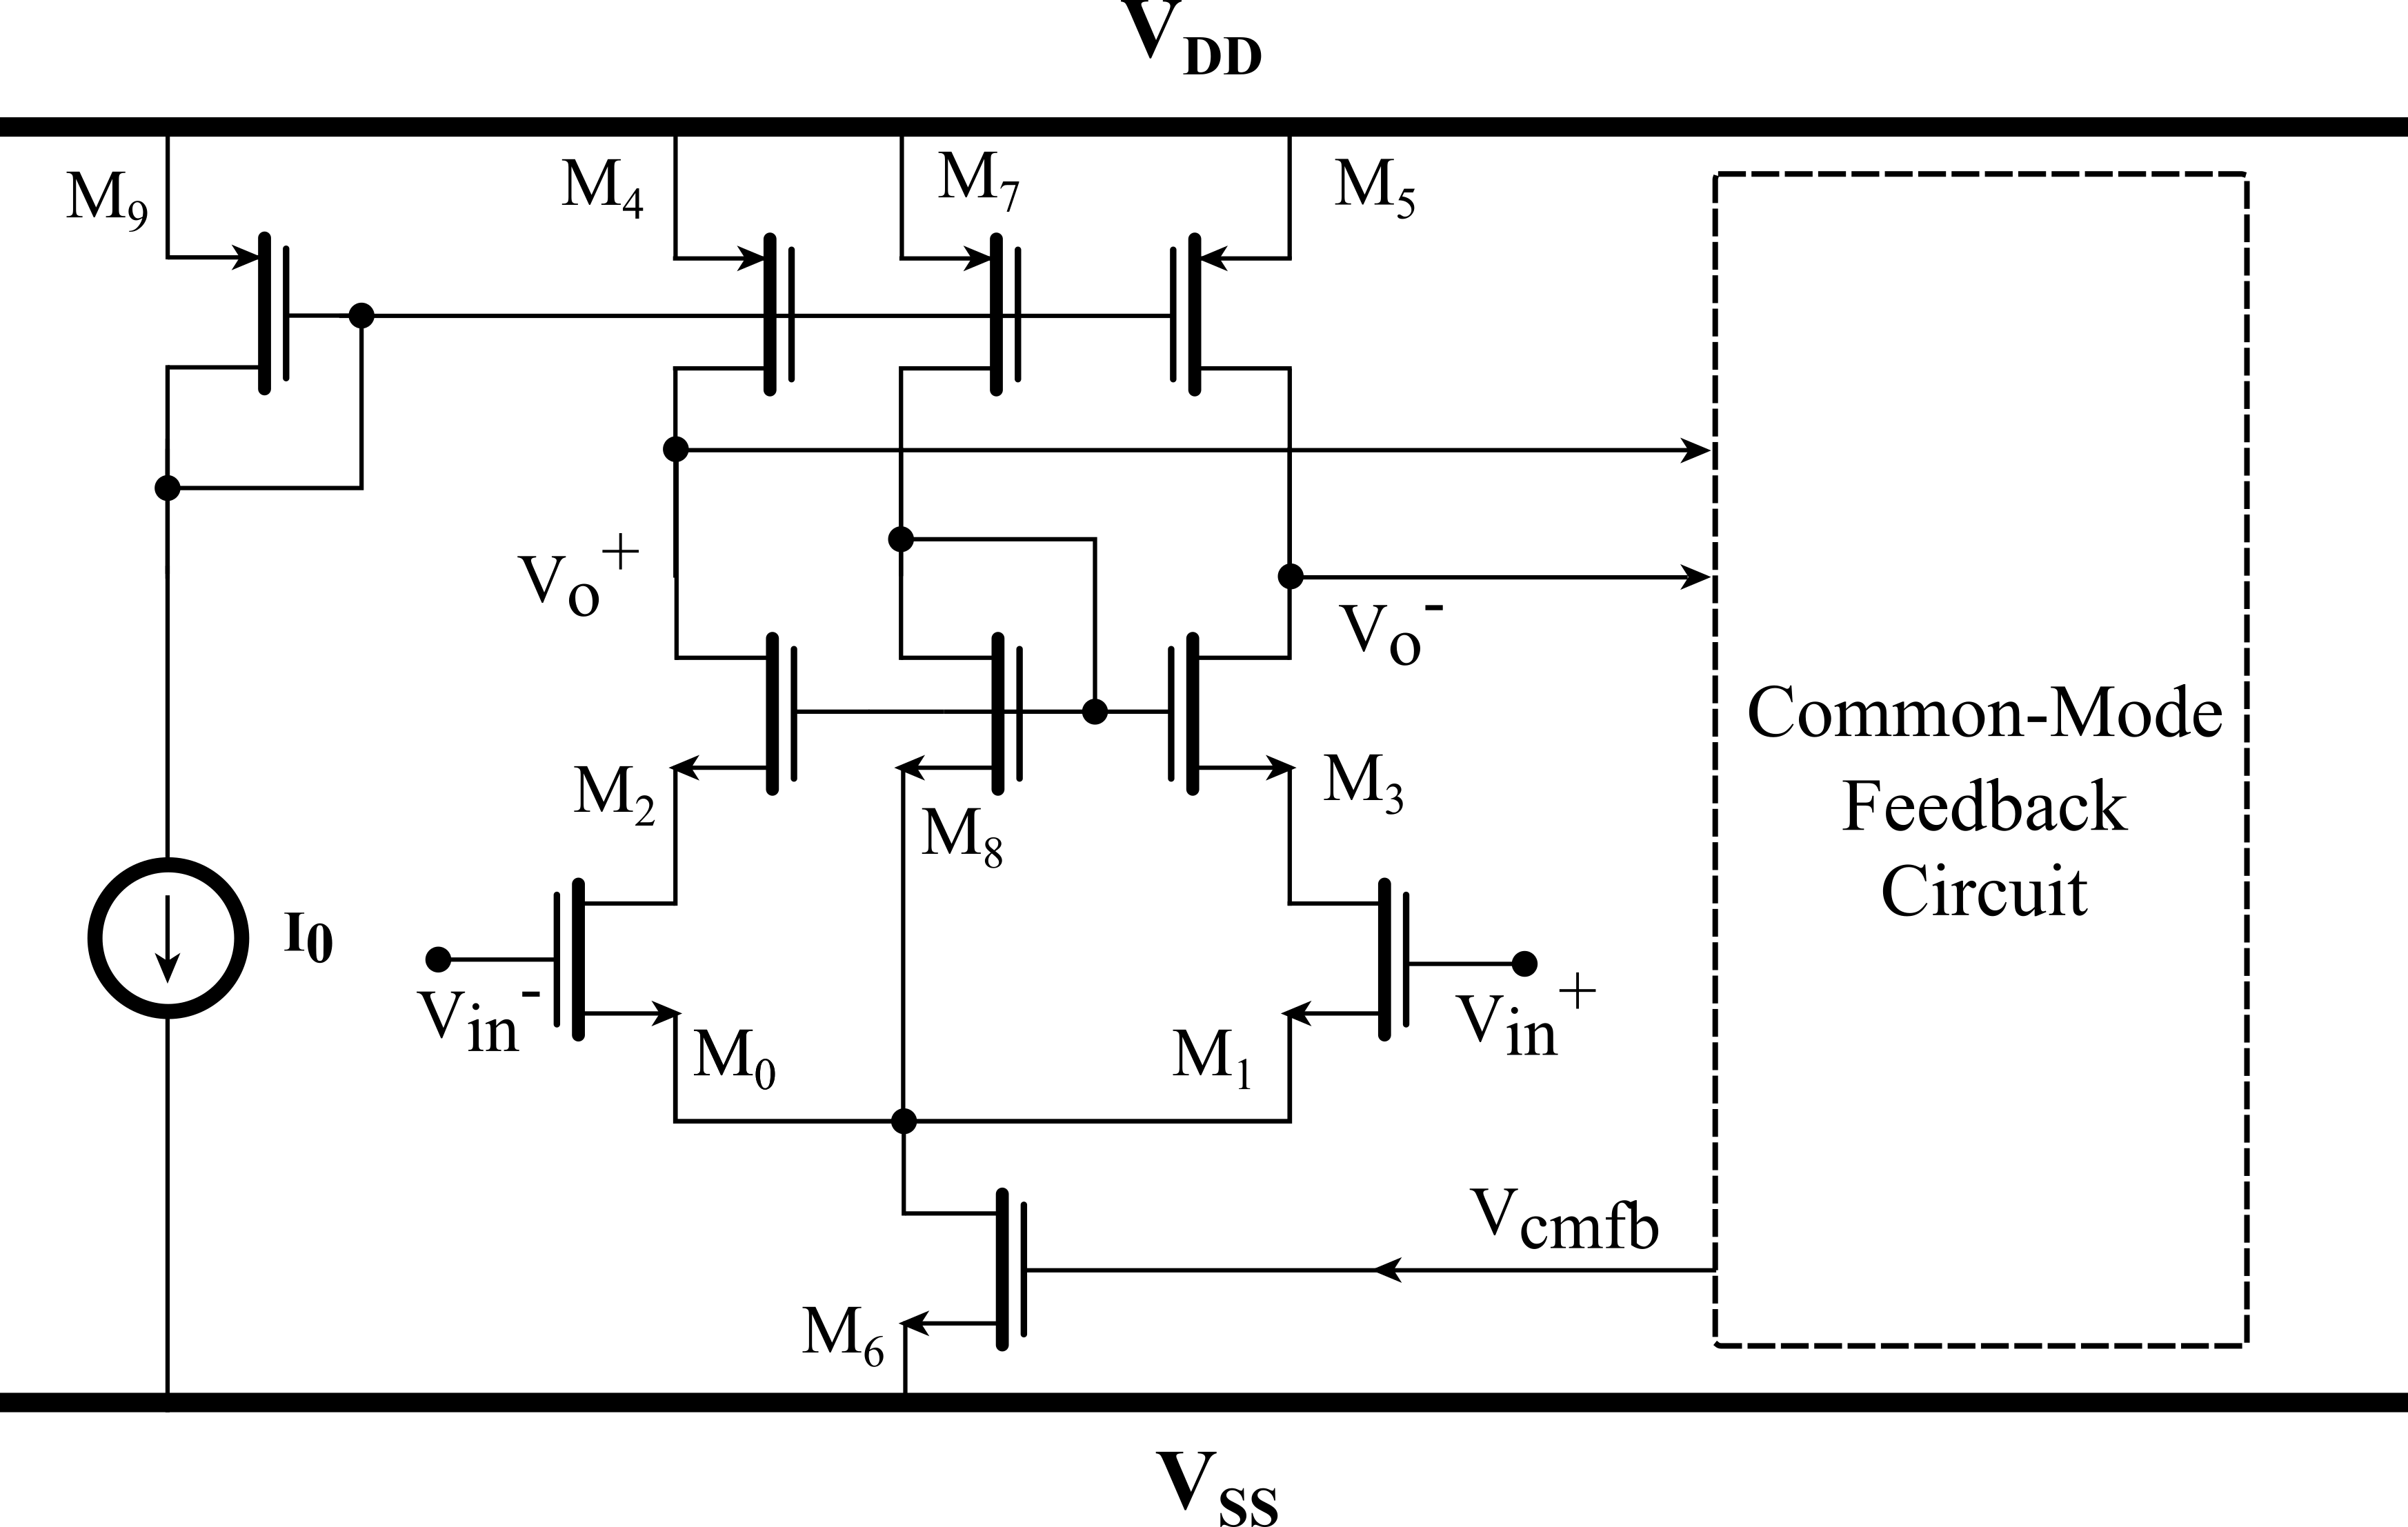
\includegraphics[width=0.9\columnwidth]{Chap05/Figures/telescopic_m.png}
\caption{Modified Telescopic Amplifier for improved output swing}
\label{TELE_AMP1}
\end{figure}
%
Two stage op-amps usually consumes more power compared to single stage op-amps, therefore the choice of single stage op-amp is made. But reduction in power comes with a drawback of reduced low frequency gain. Telescopic amplifier is the suitable alternative with the objective to overcome this drawback. In case of Telescopic amplifier, total five transistors are in stack from rail to rail (two transistors more compared to simple differential amplifier) which limits the output swing by two overdrives w.r.t. single stage differential amplifier as shown in Fig. \ref{fig:TELE_AMP}. The approach to improve the output swing can be to eliminate the one transistor from the stack highlighted in conventional structure and cause to raise it by one overdrive (Fig. \ref{TELE_AMP1}). However, the elimination of the transistor in stack leads to the lowering the gain and thus necessitates to investigate the technique to resolve this problem.


The expression for the low-frequency gain of the telescopic amplifier shown in Fig. \ref{fig:TELE_AMP} is given as,
%
\begin{equation}
    A_0 \approx g_{m0,1}\left(g_{m2,3}r_{O2,3}r_{O0,1}||g_{m6,7}r_{O6,7}r_{O4,5}\right)
\end{equation}
%
However, the elimination of the transistor from the stack reduces the output resistance, which in turn brings the low frequency gain, down. The expression for the low frequency gain and GBW of the modified telescopic amplifier for improved swing,
%
\begin{equation}\label{eq:A_0_swing_improve}
    A_0 \approx g_{m0,1}\left(g_{m2,3}r_{O2,3}r_{O0,1}||r_{O4,5}\right)
\end{equation}
%
%
\begin{equation}
    GBW = \frac{g_{m0,1}}{2\pi C_L}
\end{equation}
%
\subsection{Gain and GBW Enhancement:}
A technique is employed where the Auxiliary op-amp is incorporated for the purpose of gain enhancement\cite{ISCAS_PEREZ} as shown in the block diagram Fig. \ref{BLK_GIN_ENH}. Auxiliary op-amp takes same inputs as the principal one and generates the signals which in turns, are used to drive the main op-amp. The power consumption of the auxiliary op-amp is significantly lower than that in the principal one.
\begin{figure}[h]
\centering
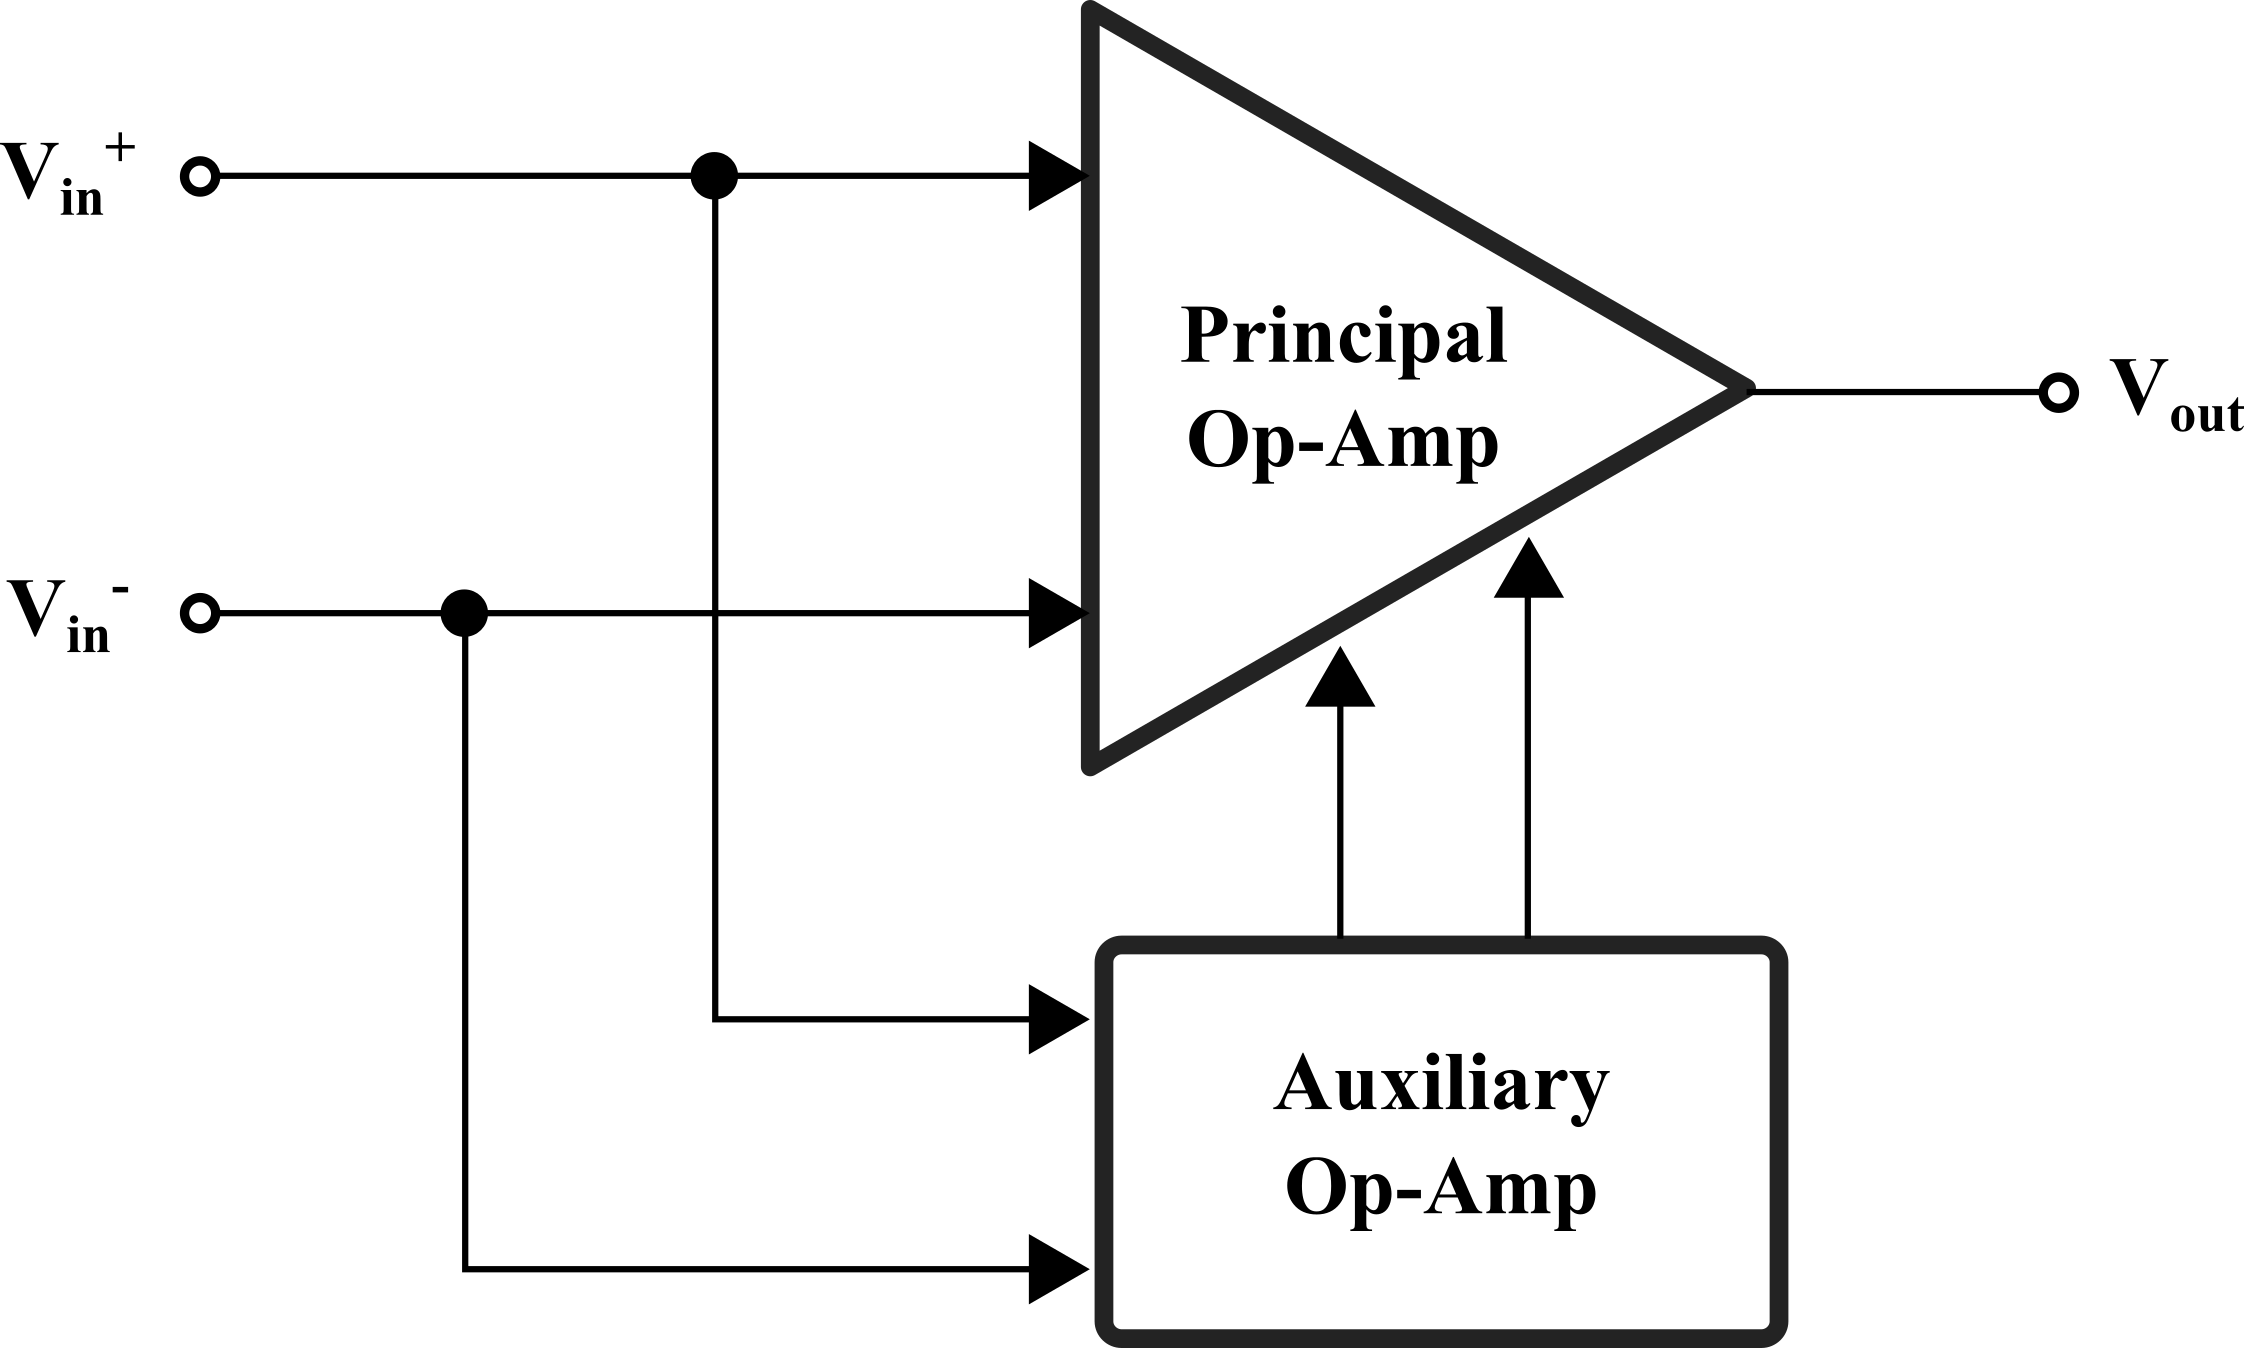
\includegraphics[width=0.6\columnwidth]{Chap05/Figures/block_diagram_gain_enhancement.png}
\caption{Block Diagram of Gain and GBW Enhancement}
\label{BLK_GIN_ENH}
\end{figure}

The circuit level implementation of the architecture is as shown in the Fig. \ref{fig:GIN_ENH_TELE_AMP}. The Auxiliary op-amp is a single stage differential amplifier with diodes as a load. The diode connected loads $M_{a2}$ and $M_{a3}$ in the Auxiliary op-amp are used to bias the current sources $M_5$ and $M_4$ in the principal op-amp respectively as shown in the Fig. \ref{fig:GIN_ENH_TELE_AMP}. With this architecture of the amplifier, all the requirements for the first integrator are fulfilled.

The bias voltages to the current sources in modified architecture for improved swing are fixed as shown in Fig. \ref{TELE_AMP1}. In case of Gain-enhanced telescopic architecture, the bias voltages $v_A$, $v_B$ are generated from auxiliary op-amp and are not constant. These voltages change as the input changes and are applied to the controlled current sources. The signal voltage $v_A$ is applied to transistor $M_4$ and $v_B$ to $M_5$.

\begin{figure}[ht]
\centering
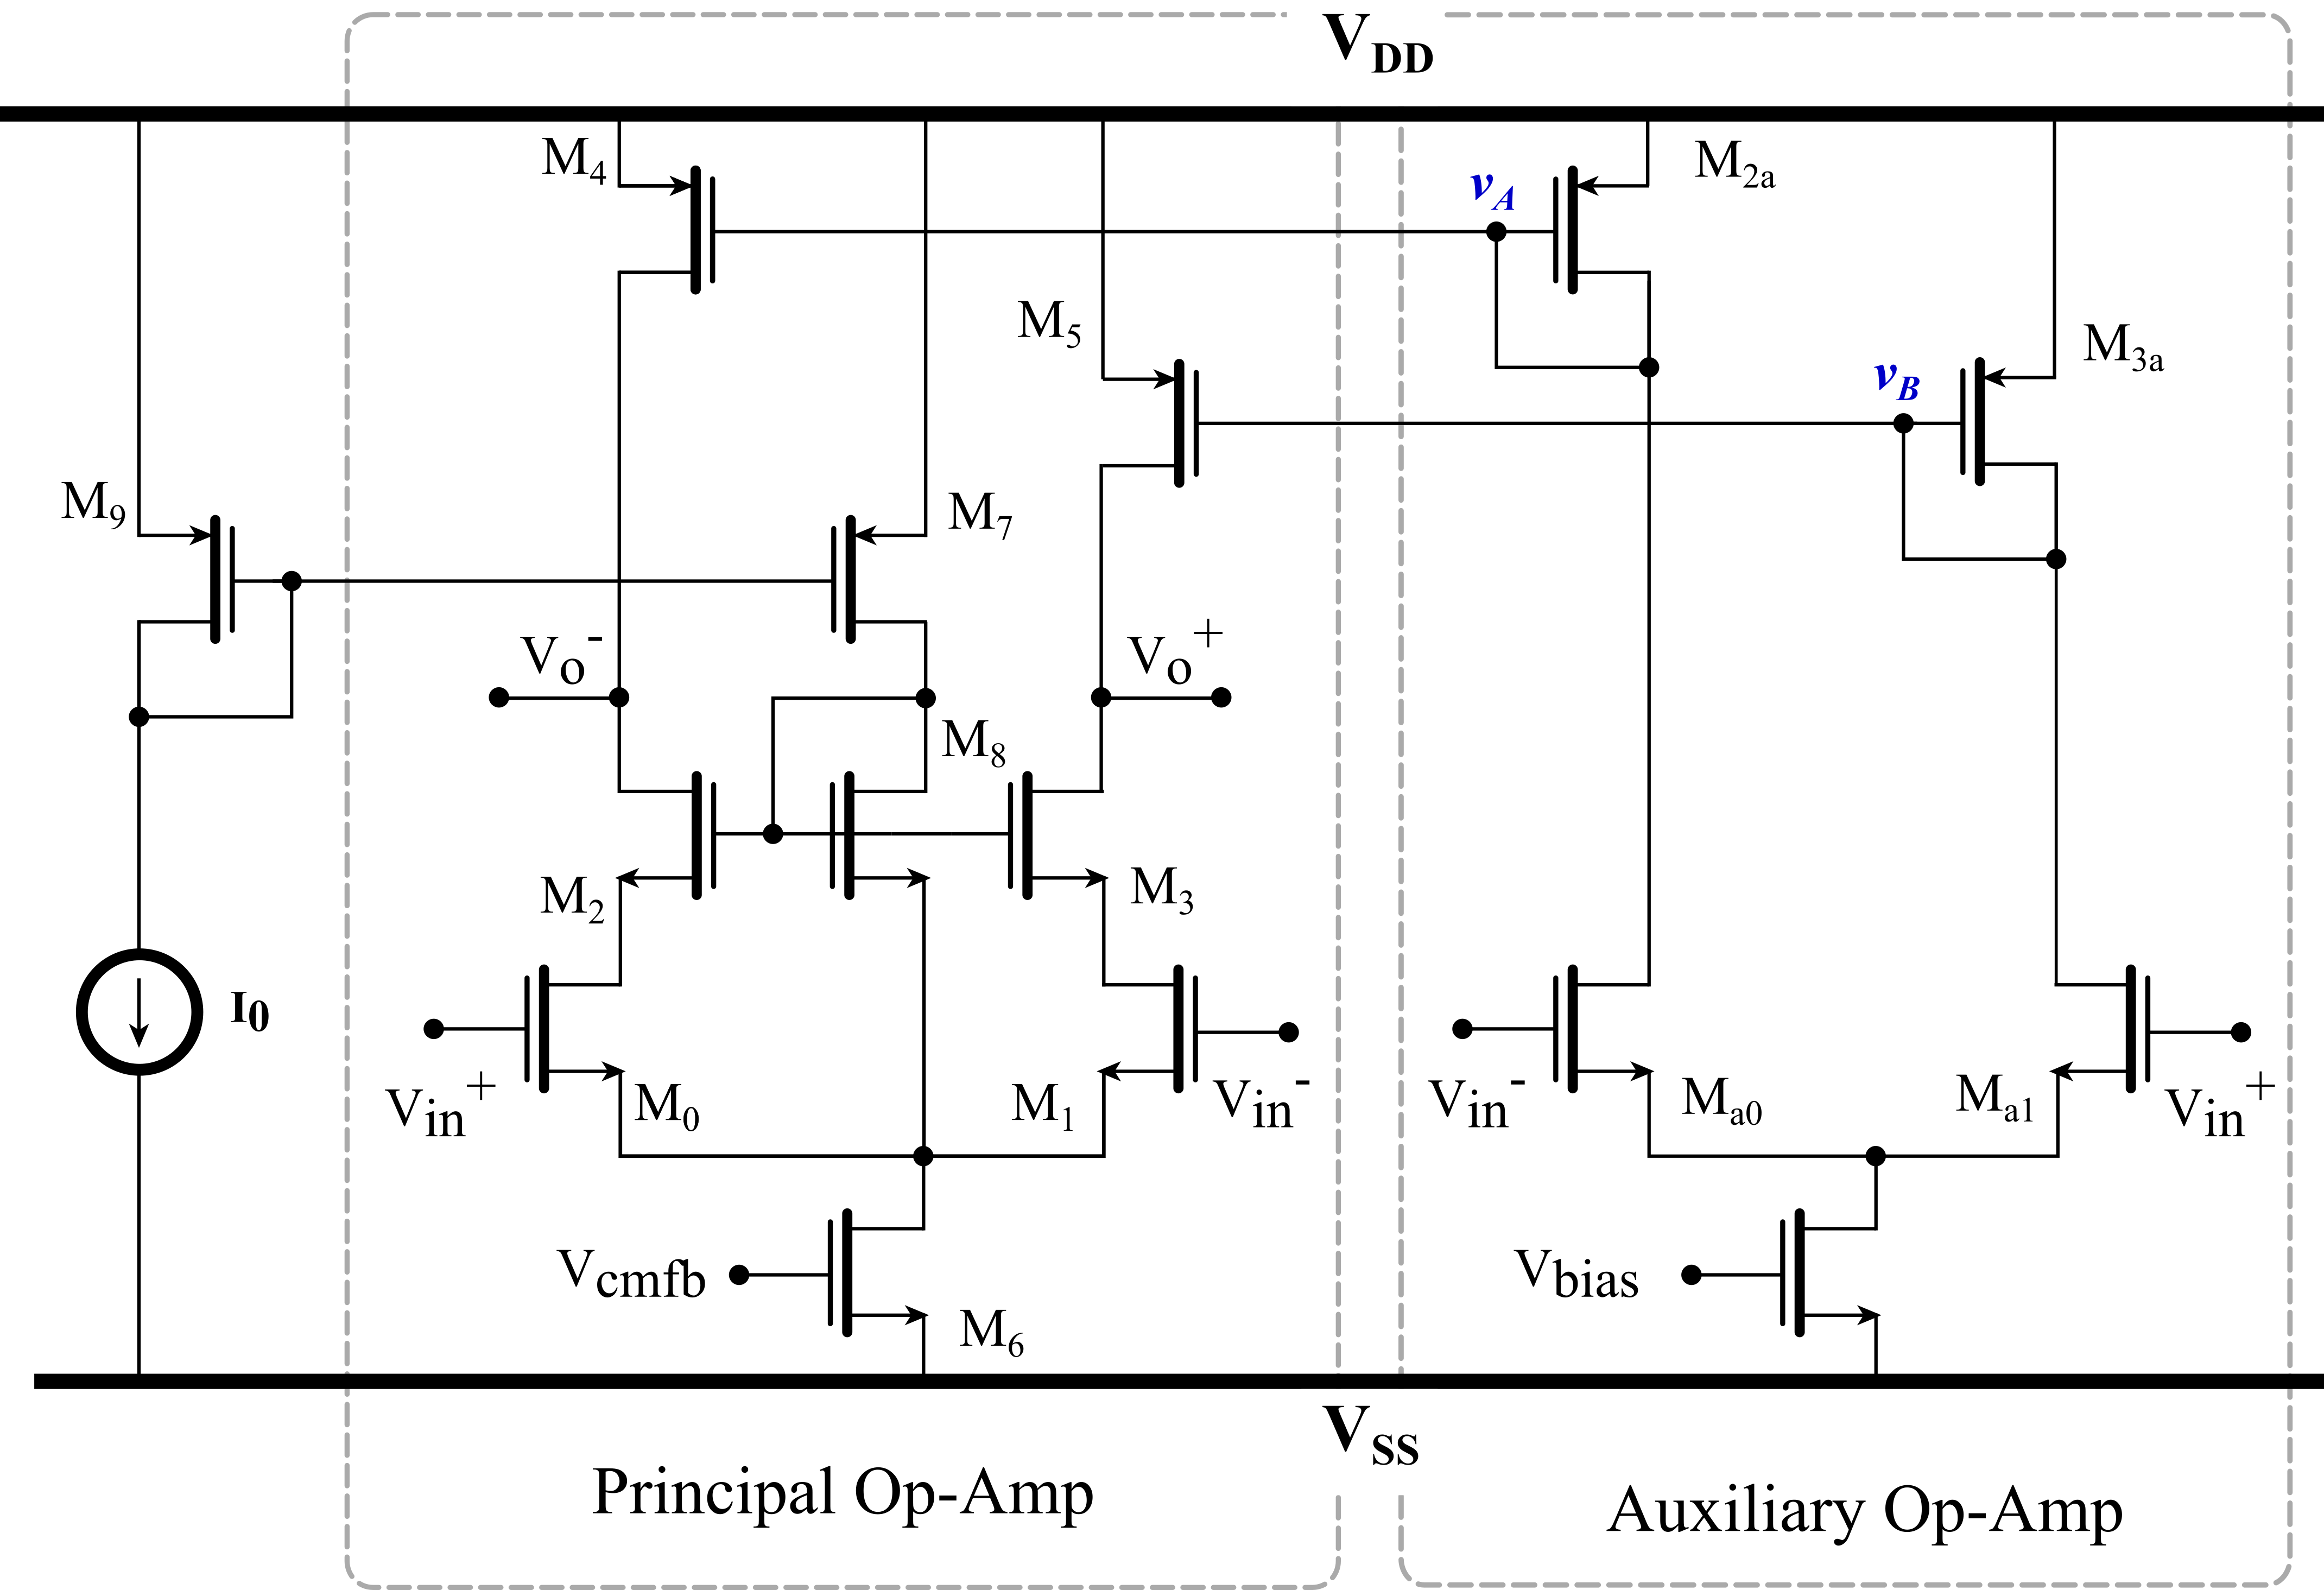
\includegraphics[width=\columnwidth]{Chap05/Figures/gain_enhanced_telescopic.png}
\caption{Gain enhanced Telescopic Amplifier for improved output swing with GBW boost(Common-Mode Feedback circuit not shown)}
\label{fig:GIN_ENH_TELE_AMP}
\end{figure}

Then the expression for $v_A$ and $v_B$ can be given as,
%
\begin{equation}
    v_A = \left(\frac{g_{ma0,a1}}{g_{ma2,a3}}\right) v_{in}^+
\end{equation}
%
%
\begin{equation}
    v_B = \left(\frac{g_{ma0,a1}}{g_{ma2,a3}}\right) v_{in}^-
\end{equation}
%
Now, in the principal op-amp, because of the input signal $v_{in}^+$ and $v_{in}^-$, the current modulation in transistor $M_0$ is $i_0=g_{m0,1}v_{in}^+$ while that in transistor $M_1$ is $i_1=g_{m0,1}v_{in}^-$ that flows through the output resistance, where output resistance is given by,
%
\begin{equation}
    r_{out} = g_{m2,3}r_{O2,3}r_{O0,1}||r_{O4,5}
\end{equation}
%
Furthermore, the non-constant voltages $v_A$ and $v_B$ also causes the further modulation in the output currents through $M_4$ and $M_5$. The expressions of these currents can be given as,
%
\begin{equation}
    i_4 = g_{m4}v_A = g_{m4,5}\left(\frac{g_{ma0,a1}}{g_{ma2,a3}}\right) v_{in}^+
\end{equation}
%
%
\begin{equation}
    i_5 = g_{m5}v_B = g_{m4,5}\left(\frac{g_{ma0,a1}}{g_{ma2,a3}}\right) v_{in}^-
\end{equation}
%

Then the output voltage of the principal op-amp is expressed as,
%
\begin{equation}
    \begin{split}
        v_{out} &= v_{out}^+ - v_{out}^-\\
                &= (i_0+i_4)r_{out} - (i_1+i_5)r_{out}\\
                &= \left\{\left[g_{m0,1}v_{in}^++g_{m4,5}\left(\frac{g_{ma0,a1}}{g_{ma2,a3}}\right) v_{in}^+\right]-\left[g_{m0,1}v_{in}^-+g_{m4,5}\left(\frac{g_{ma0,a1}}{g_{ma2,a3}}\right) v_{in}^-\right]\right\}r_{out}\\
                &=\left(g_{m0,1}+g_{m4,5}\frac{g_{ma0,a1}}{g_{ma2,a3}}\right)r_{out}\left(v_{in}^+ - v_{in}^-\right)
    \end{split}
\end{equation}
%
And therefore, low-frequency gain is represented as,
%
\begin{equation}\label{eq:A0_gain_enhanced}
\begin{split}
    A_0 &= \frac{v_{out}}{v_{in}}=\frac{\left(v_{out}^+ - v_{out}^-\right)}{\left(v_{in}^+ - v_{in}^-\right)}\\ 
        &= \left(g_{m0,1}+g_{m4,5}\frac{g_{ma0,a1}}{g_{ma2,a3}}\right)r_{out}\\
        &=\left(g_{m0,1}+g_{m4,5}\frac{g_{ma0,a1}}{g_{ma2,a3}}\right)\left(g_{m2,3}r_{O2,3}r_{O0,1}||r_{O4,5}\right)
\end{split}
\end{equation}
%
%
\begin{figure}[t]
\centering
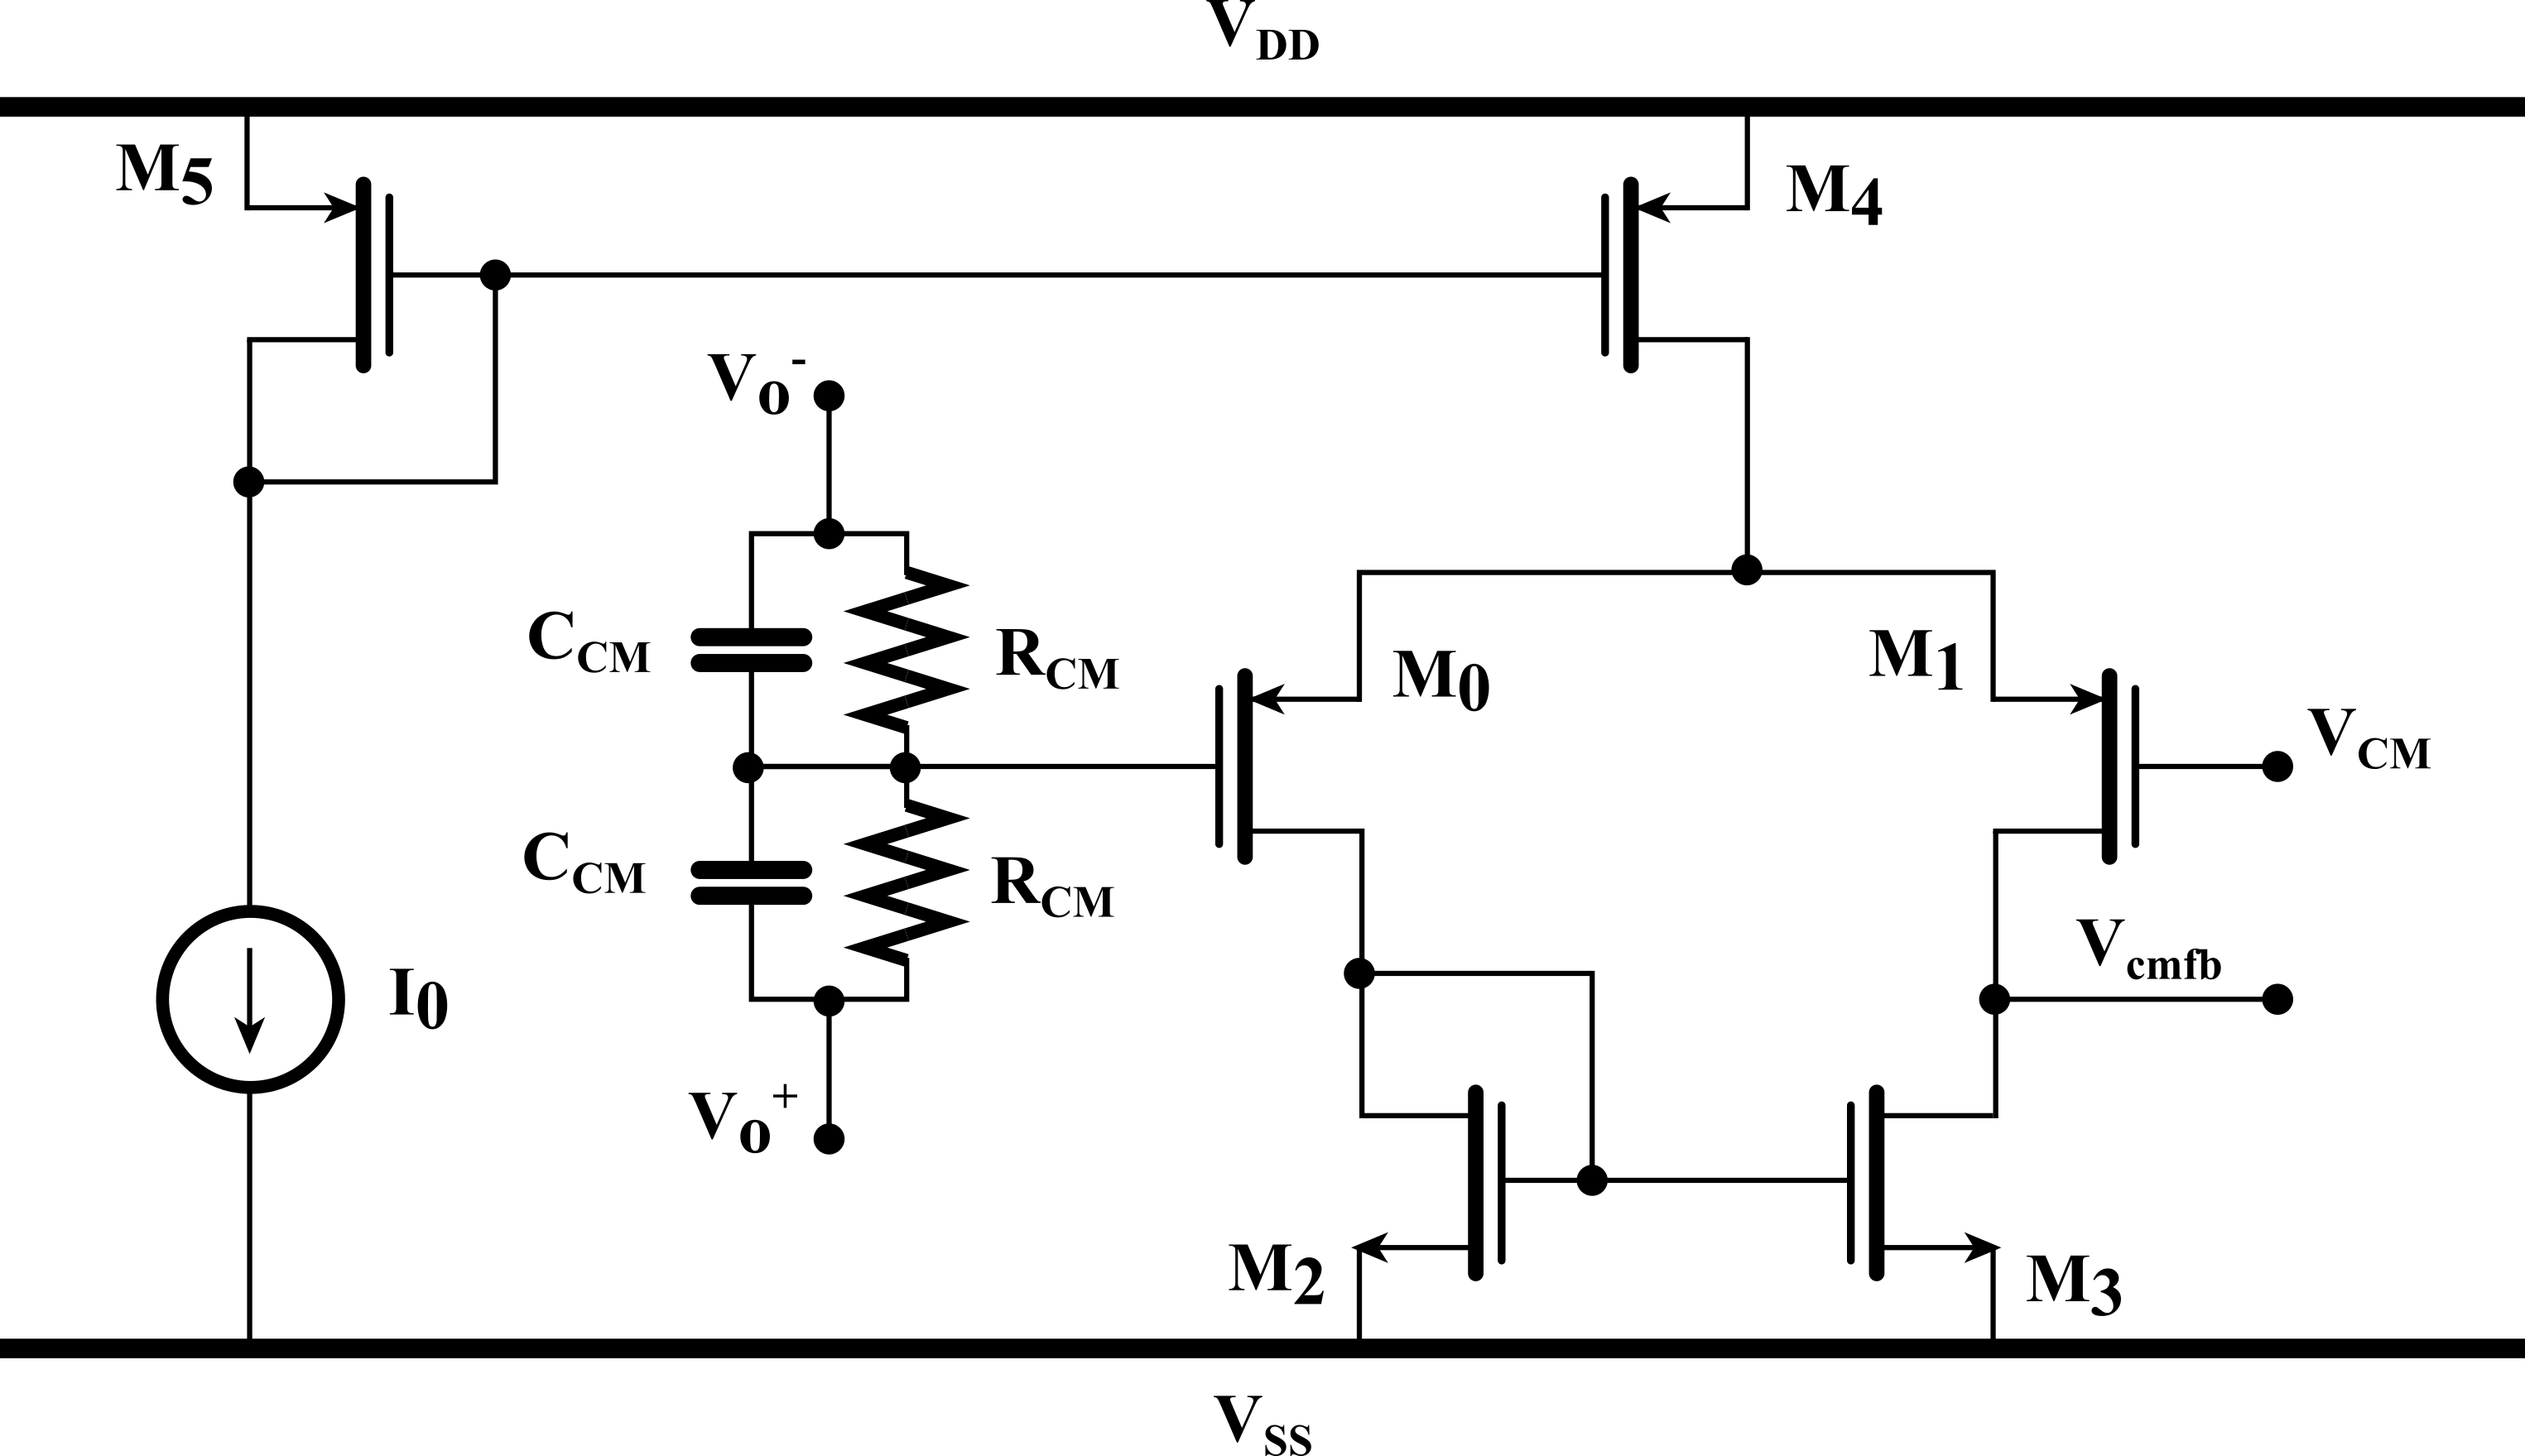
\includegraphics[width=0.8\columnwidth]{Chap05/Figures/common_mode_feedback.png}
\caption{Conventional continuous time Common-Mode Feedback Circuit}
\label{fig:COMMON_MODE}
\end{figure}
%
Eq. (\ref{eq:A_0_swing_improve}) represents the low frequency gain of the modified telescopic amplifier for swing improvement where the transconductance of the structure is $G_m = g_{m0,1}$. While that of the Gain-enhanced telescopic amplifier can be given as, from Eq.(\ref{eq:A0_gain_enhanced}),
%
\begin{equation}
    G_m = g_{m0,1}+g_{m4,5}\frac{g_{ma0,a1}}{g_{ma2,a3}}
\end{equation}
%
It is clear from the equation above that, the scaled transconductance of transistor $M_4$ ($M_5$) is added to the $g_{m0,1}$ boosting it's gain. The GBW also gets raised as a result increase in the transconductance.

%
\begin{figure}[]
\centering
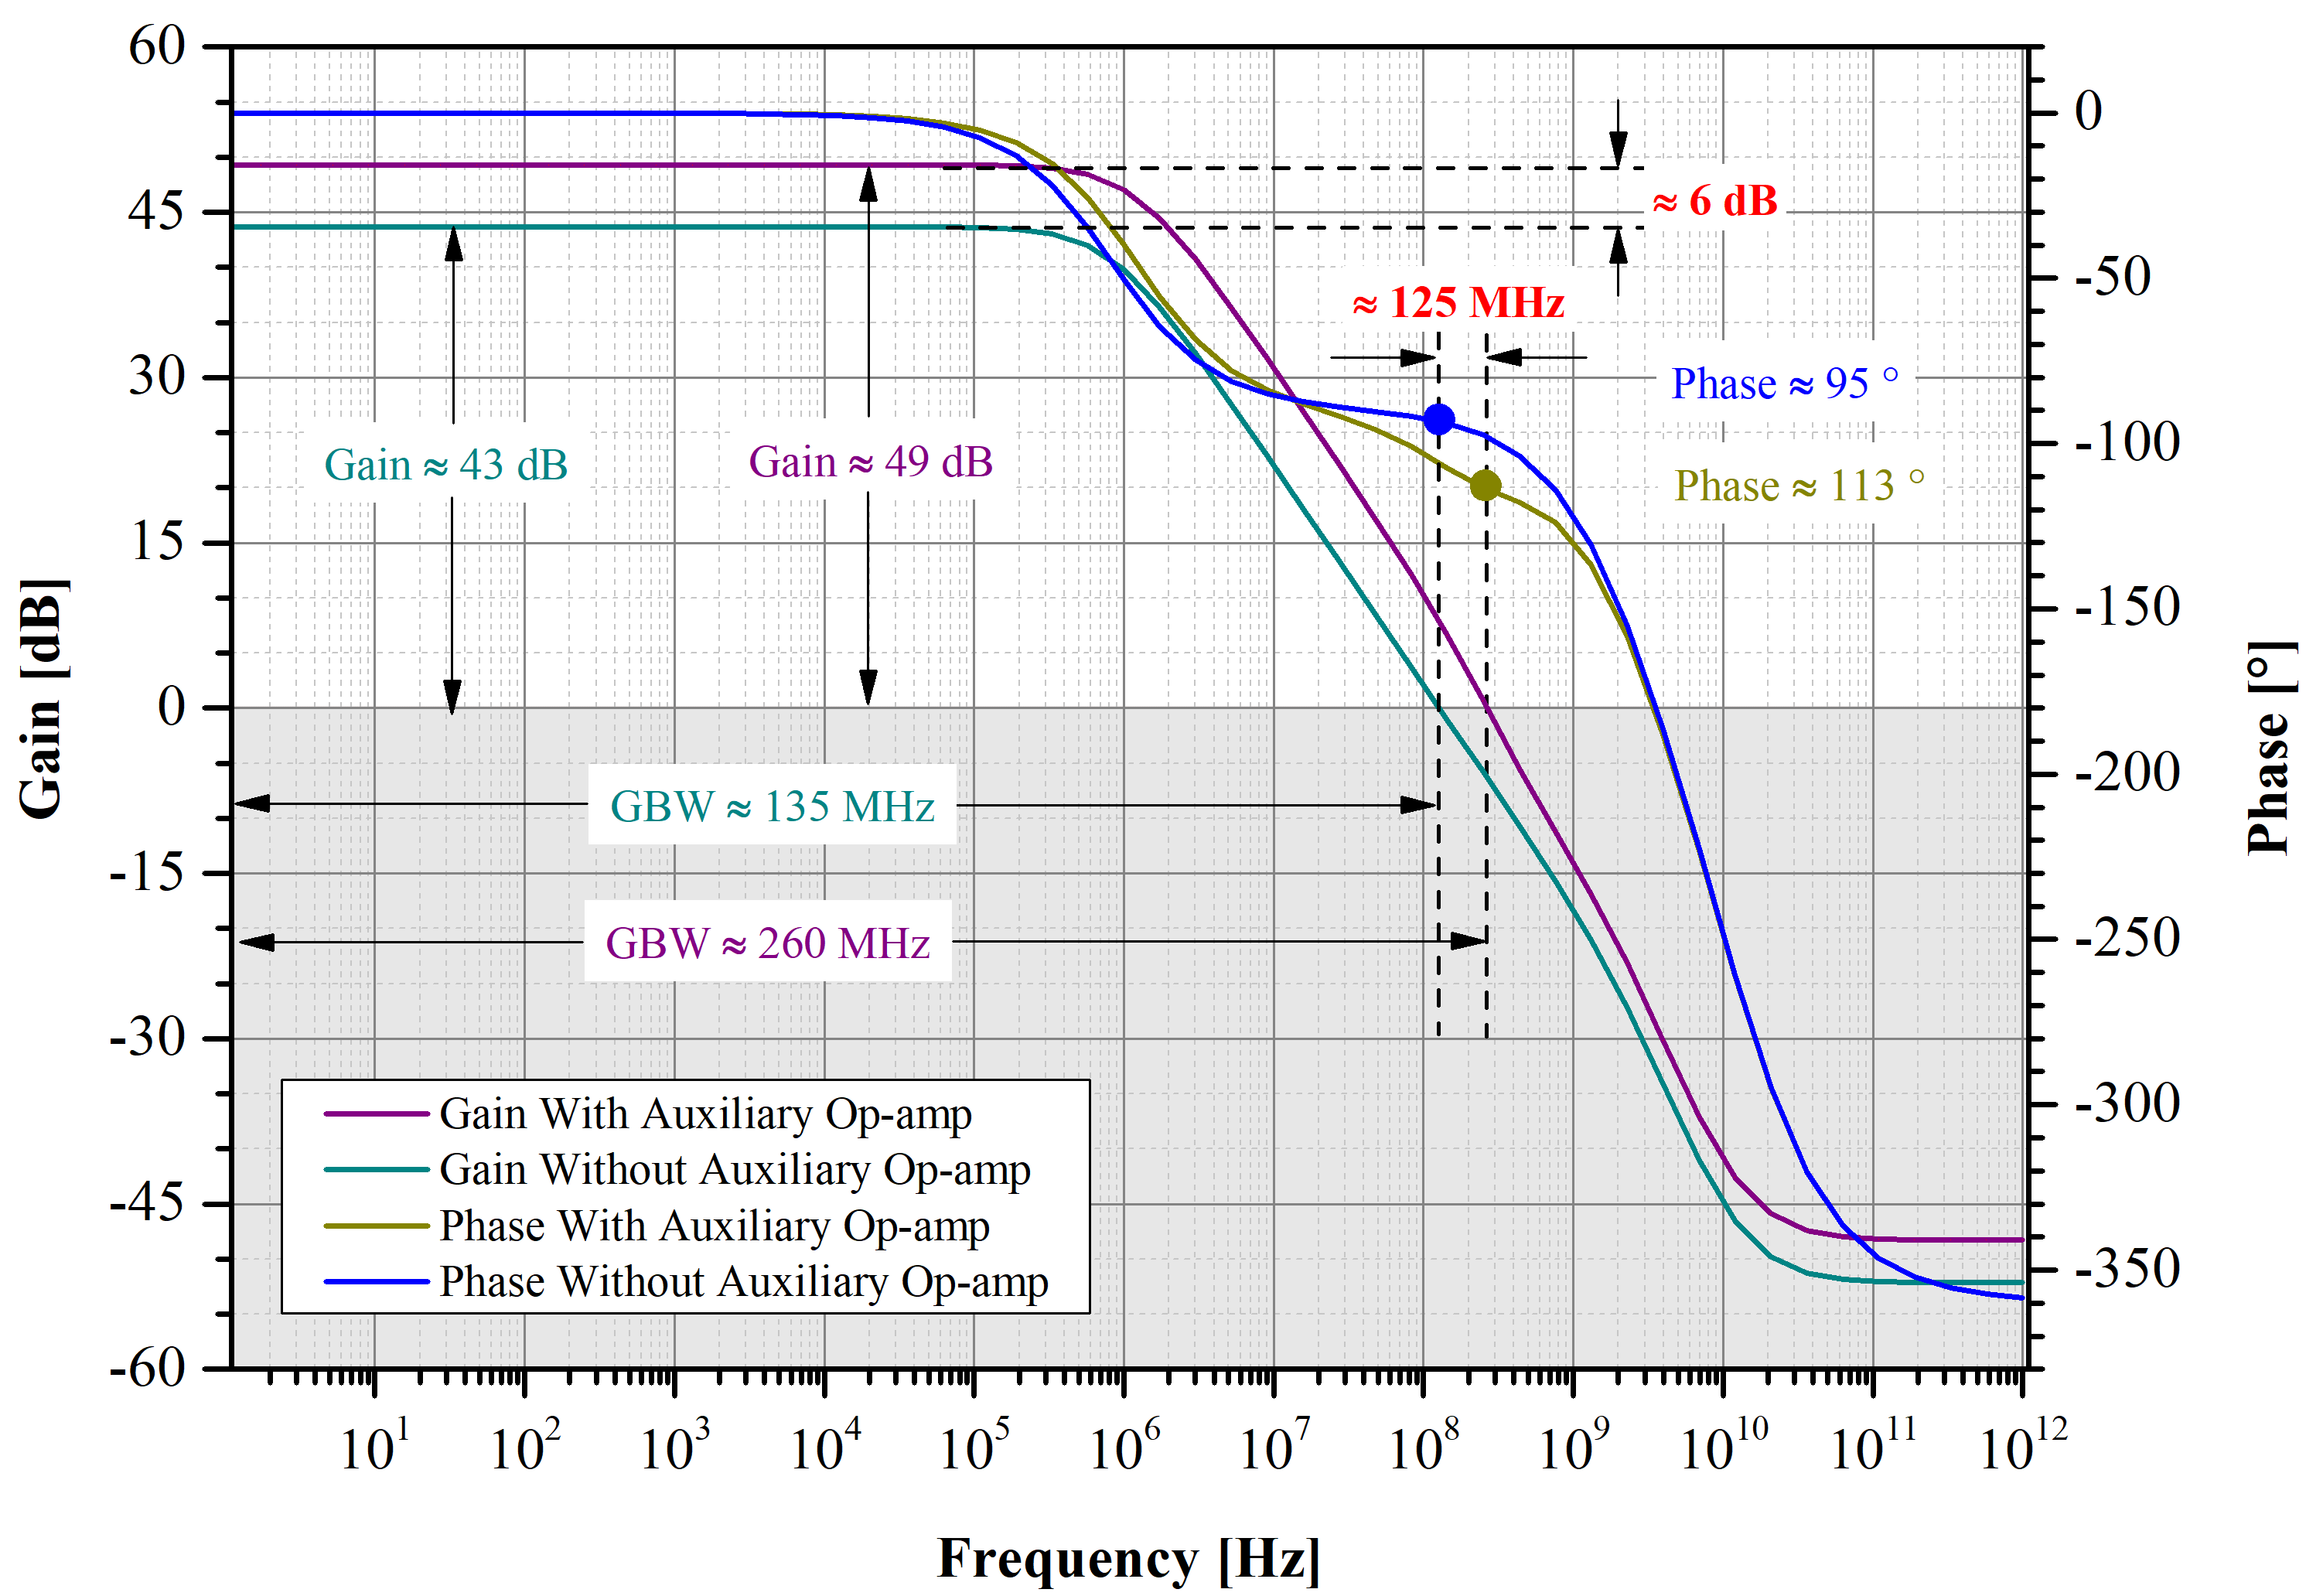
\includegraphics[width=\columnwidth]{Chap05/Figures/gain_gbw_comparison.png}
\caption{Frequency Response comparison between the modified Telescopic amplifier architectures with and without the Auxiliary op-amp for the first integrator}
\label{fig:gain_gbw_comparison}
\end{figure}
%
%
\begin{equation}
\begin{split}
        GBW &= \frac{\left(g_{m0,1}+g_{m4,5}\frac{g_{ma0,a1}}{g_{ma2,a3}}\right)}{2\pi C_L} \\
            &= \left(1+\frac{g_{m4,5}}{g_{m0,1}}\frac{g_{ma0,a1}}{g_{ma2,a3}}\right)\frac{g_{m0,1}}{2\pi C_L}
\end{split}
\end{equation}
%

The Fig.\ref{fig:gain_gbw_comparison} shows the schematic simulation results comparison between the architectures of the modified telescopic amplifiers without auxiliary op-amp (Fig. \ref{TELE_AMP1}) and with auxiliary op-amp (Fig. \ref{fig:GIN_ENH_TELE_AMP}). The gain characteristic and the phase characteristics are plotted as a function of frequency for the modified architecture of telescopic amplifier with and without the auxiliary op-amp. 

In case of the modified architecture of telescopic amplifier for improved swing without auxiliary op-amp, the low frequency gain attained is around 43~dB, gain-bandwidth product is around 135~MHz and the phase margin is 85~° (180-95). While, when an auxiliary op-amp is incorporated to bias the current sources of principal op-amp, the achieved low frequency gain increases to 49~dB, GBW increases to around 260~MHz with phase margin of around 67~°. For the 135~MHz of given GBW, the op-amp architecture without auxiliary op-amp consumes a current of 470~µA, while the op-amp architecture with auxiliary op-amp consumes just 500~µA of current (470~µA in the principal op-amp and 30~µA in the auxiliary op-amp) boosting the gain by 6~dB and GBW by 125~MHz, i.e. there is almost 100\% increase in the gain as well as GBW with just nominal amount of extra current consumption of just 6-7\% (30~µA).
%
\begin{figure}[h!]
\centering
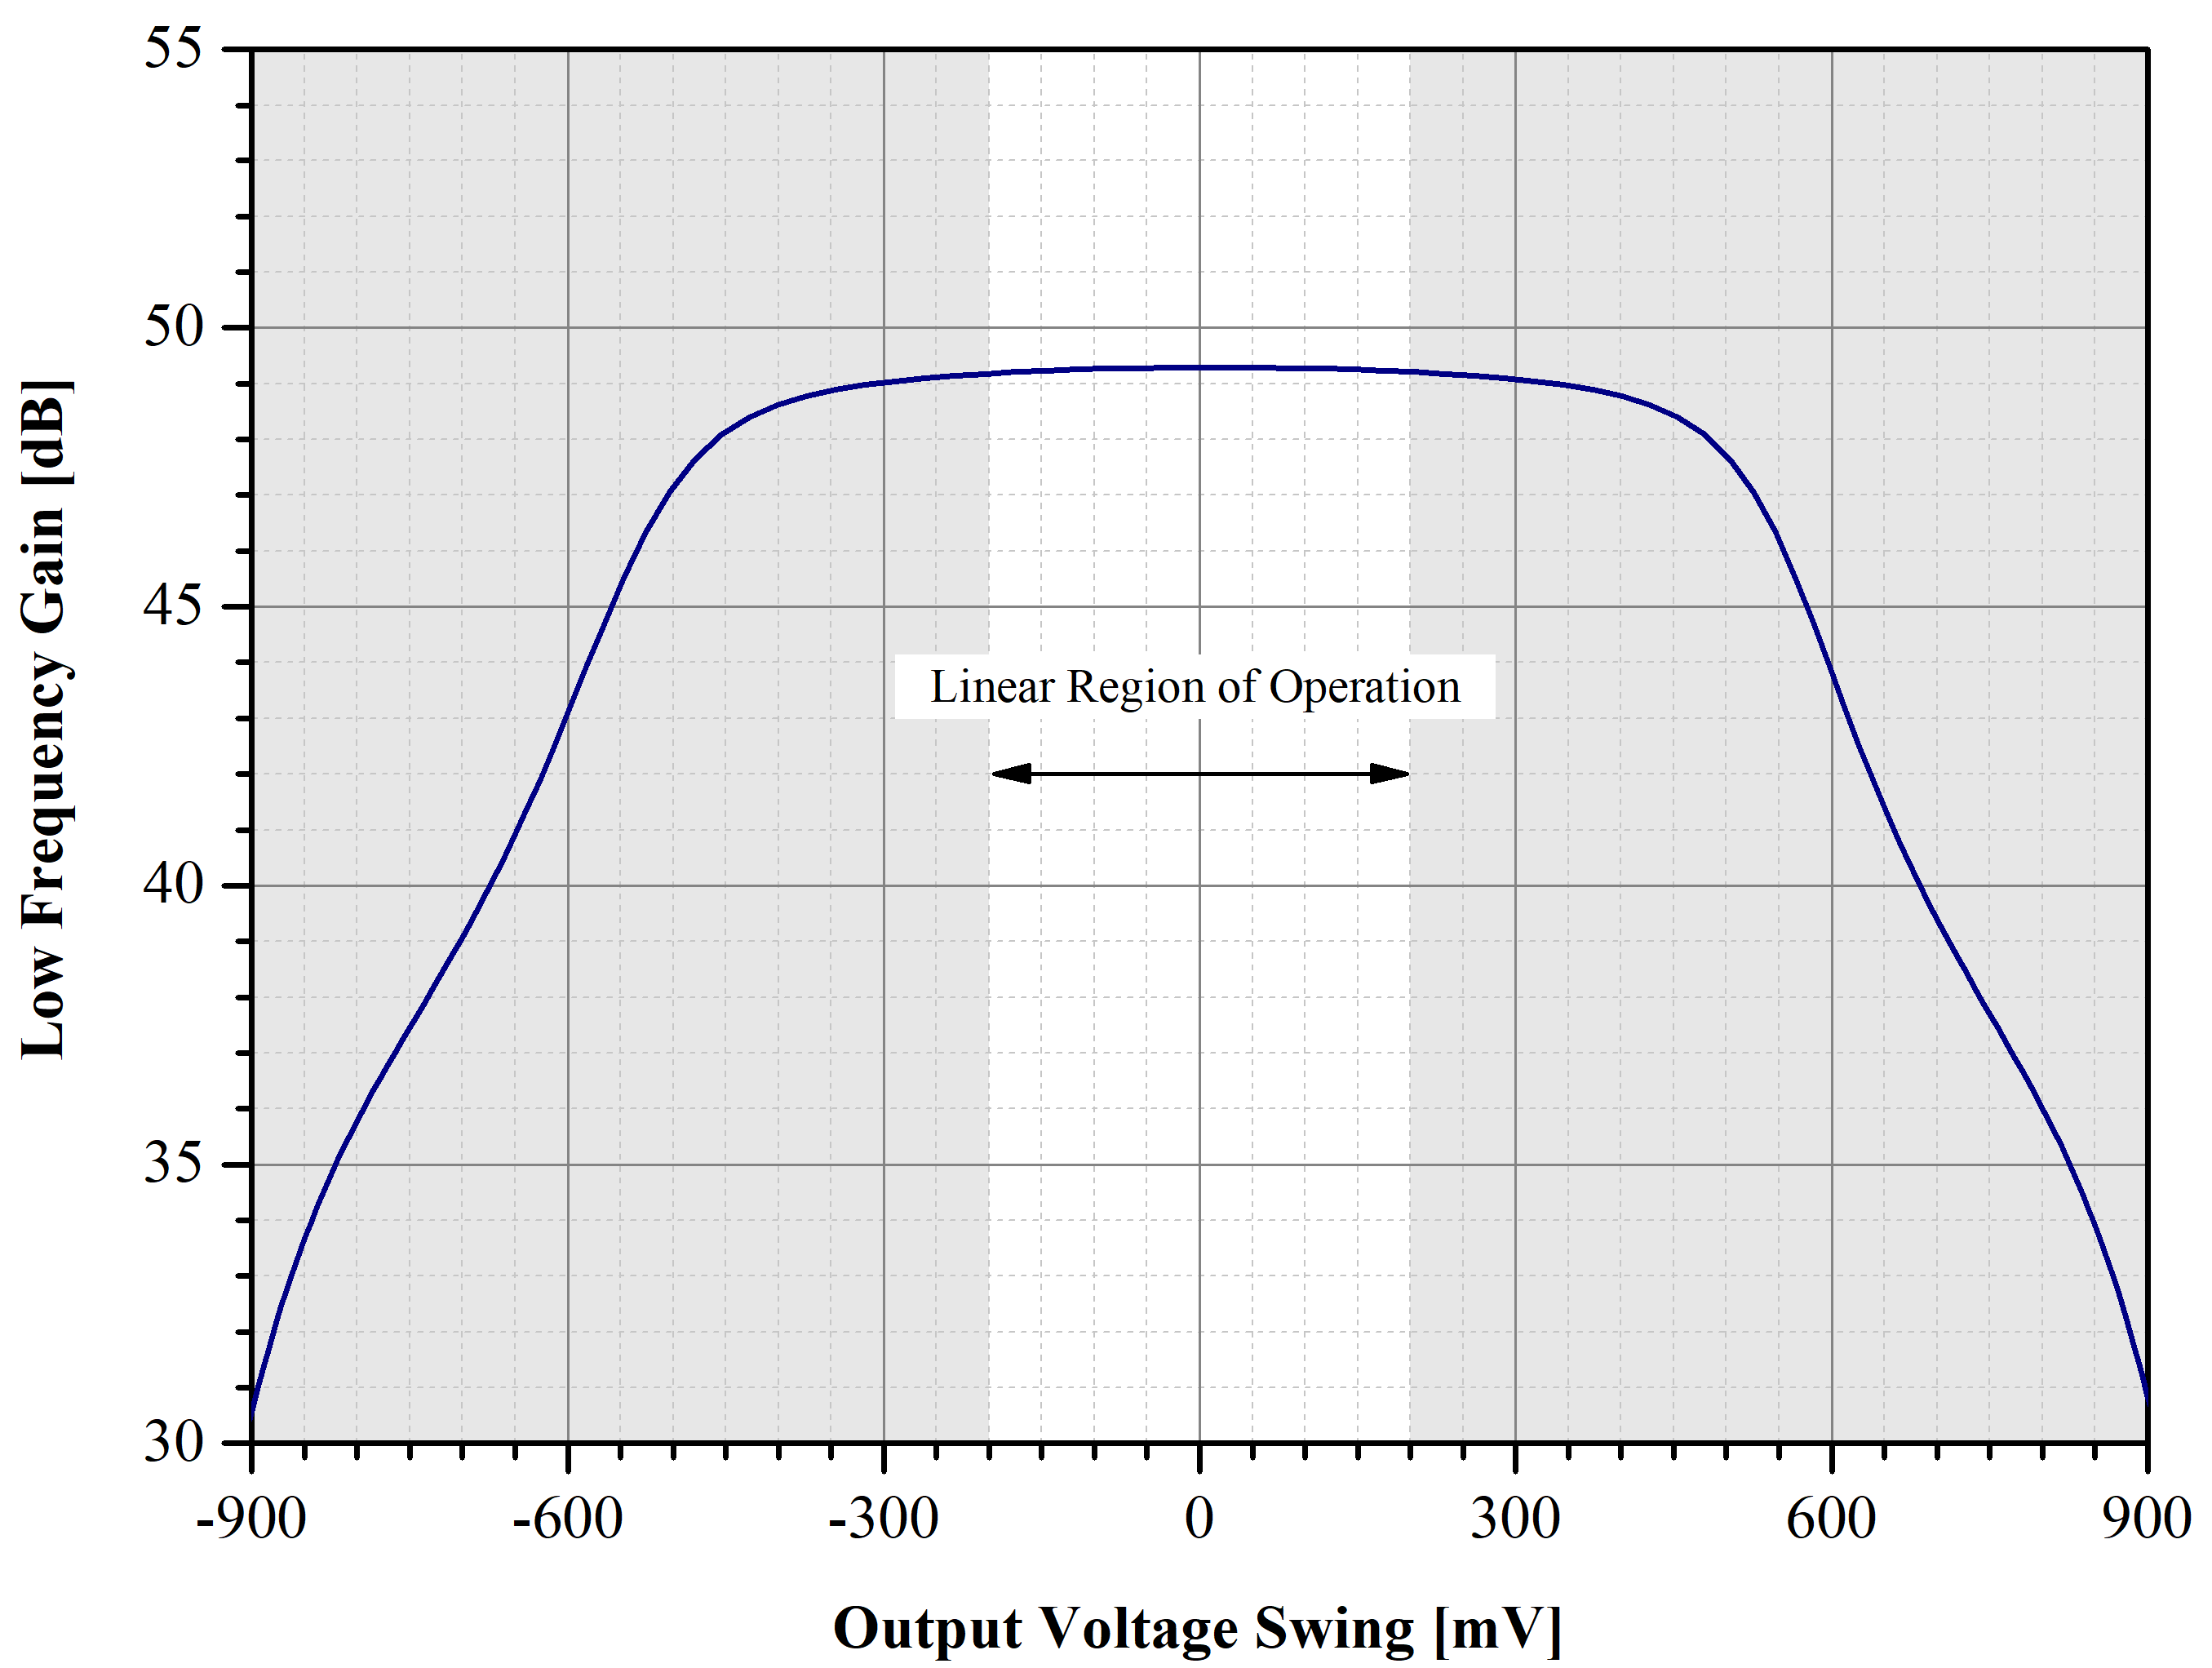
\includegraphics[width=0.9\columnwidth]{Chap05/Figures/gain_vs_swing.png}
\caption{Output swing of the Op-amp Vs low frequency gain}
\label{fig:gain_vs_swing}
\end{figure}
%

Next, the analysis of output voltage swing of the op-amp architecture has also been done having considered the constant voltage gain region. The low frequency gain is plotted as a function of differential output voltage swing as shown in Fig. \ref{fig:gain_vs_swing}. It is clear from the figure that the low frequency gain is around 50~dB at 0~mV differential output voltage and remains constant for output voltage from -300~mV to +300~mV exhibiting the swing of 600~mV deferentially.
% Please add the following required packages to your document preamble:
% \usepackage{multirow}
\begin{table}[]
\centering
\begin{tabular}{c|c|c|c}
\Xhline{4\arrayrulewidth}
\multirow{2}{*}{\textbf{Transistor}} & \textbf{First Op-amp} & \textbf{Second Op-amp} &        \\ \cline{2-3} 
                            & W (\textmu m)  & W (\textmu m)  & L (\textmu m) \\ \hline
M\textsubscript{0,1}                        & 60      & 40      & 0.4    \\ 
M\textsubscript{2,3}                        & 45      & 30      & 0.4    \\ 
M\textsubscript{4,5}                        & 75      & 50      & 0.4    \\ 
M\textsubscript{6}                          & 120     & 75      & 0.4    \\ 
M\textsubscript{7}                          & 5       & 5       & 0.4    \\ 
M\textsubscript{8}                          & 5       & 5       & 2.0      \\ \hline
M\textsubscript{a0,a1}                      & 4       & 4       & 0.4    \\ 
M\textsubscript{a2,a3}                      & 6       & 6       & 0.4    \\ 
M\textsubscript{a4}                         & 8       & 8       & 0.4    \\ \Xhline{4\arrayrulewidth}
\end{tabular}
\caption{Transistor sizes in the Op-amps in the first and second integrator}
\label{tab:trans_size}
\end{table}

\subsection{Op-Amp for the Second Integrator:}
Similar way the load for the second integrator can also be estimated in a phase where it has maximum amount of load which is again the integrating phase in this case. The second integrator in the feedforward and in the integrating phase appears as shown in Fig. \ref{INT2_INTPHS}. Then, from the figure, the expression for load and the feedback factor for the second integrator is pronounced in Eq. \ref{CL2} and \ref{BETA2} respectively.
\begin{figure}[h]
\centering
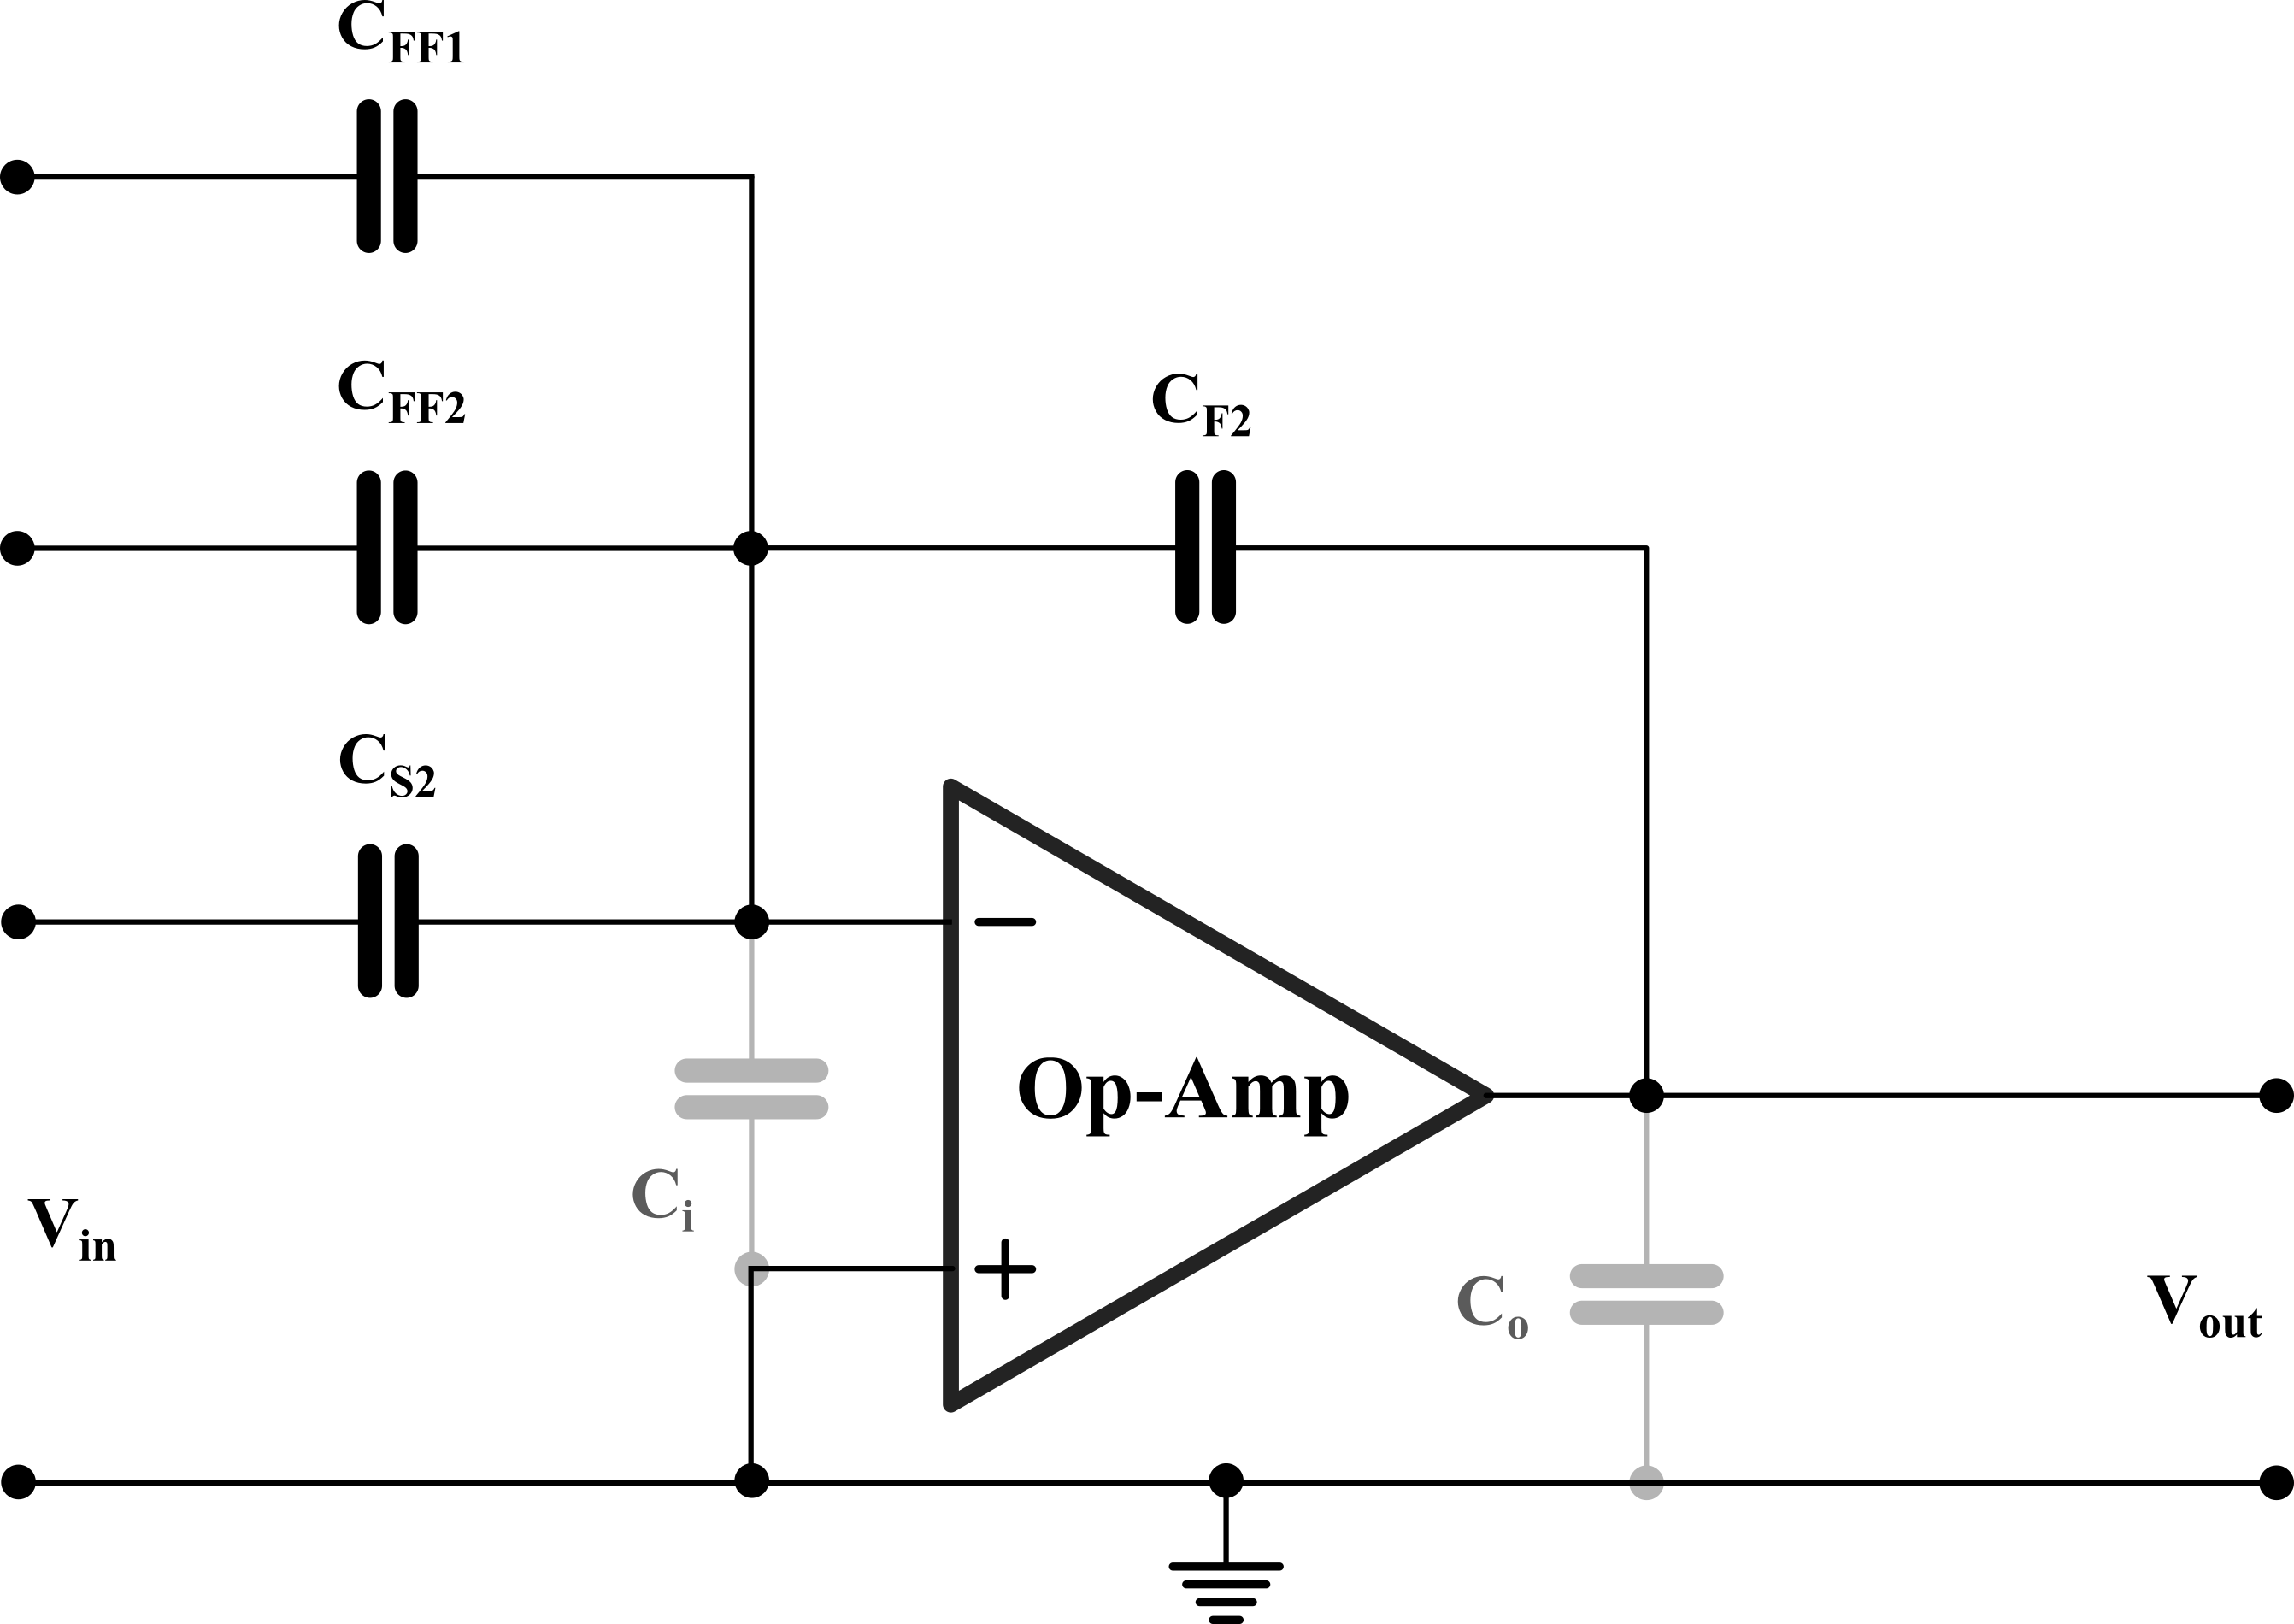
\includegraphics[width=0.6\columnwidth]{Chap05/Figures/integrator2.png}
\caption{Single Ended representation of the second Integrator in the integrating phase}
\label{INT2_INTPHS}
\end{figure}
\begin{equation}
    C_{L2}=\frac{C_{F2}\left(C_{S2}+C_{FF1}+C_{FF2}+C_{i}\right)}{C_{F2}+C_{S2}+C_{FF1}+C_{FF2}+C_{i}}+C_{o}
    \label{CL2}
\end{equation}
\begin{equation}
    \beta_{2}=\frac{C_{F2}}{C_{F2}+C_{S2}+C_{FF1}+C_{FF2}+C_{i}}
    \label{BETA2}
\end{equation}

However, in the architecture of Op-amp developed (Fig. \ref{fig:GIN_ENH_TELE_AMP}), there are four transistors stacked from positive to negative rail, while the output voltage swing requirement is 1.2~V with GBW of around 200~MHz (considering PVT variations). In order to achieve such a high GBW (even with the modified structure), it is necessary to bias the transistors in the strong inversion region, and thus at higher overdrive voltage. With these restrictions, it is quite difficult to achieve the given voltage swing. Therefore, the option is to change the coefficients of the three inputs to the second integrator by proper amount so as to accommodate the resulting signal within the voltage swing of the op-amp. Previously, the values of capacitors $C_{FF1}$, $C_{F2}$ and $C_{S2}$ were 400~fF and that of $C_{FF2}$ was 800~fF setting the coefficients, $a_2=1$, $b_1=1$ and $b_2=2$, where $a_2=\frac{C_{S2}}{C_{F2}}$, $b_1=\frac{C_{FF1}}{C_{F2}}$, $b_2=\frac{C_{FF2}}{C_{F2}}$ and as discussed, these coefficients were leading the signal swing to 1.2~V. A good scale-down coefficient could be 4 which results swing of (1.2V/4=) 300~mV and it is known that the op-amp developed for the first integrator already exhibit the same output swing, consequently which can be employed also for the op-amp in the second integrator. To do so, all the coefficients $a_2$, $b_1$ must be set to $\frac{1}{4}$ and $a_2$ must be set to $\frac{1}{2}$ which can simply be done by reducing the sizes of the input capacitors by 4. Then, final values of the capacitors are, $C_{FF1}=100~fF$, $C_{FF2}=200~fF$, $C_{S2}=100~fF$ and $C_{F2}=400~fF$.


Even in this case, the presumption for the parasitic capacitance at the virtual ground node ($C_{i}$) and the output node ($C_{o}$) is made to be around $100\ fF$. The overall load capacitor ($C_{L2}$) and the feedback factor ($\beta_2$) are computed with the help of Eq. \ref{CL2} and Eq. \ref{BETA2} and are found to be around $300~fF$ and $0.45$ respectively. Eventually similar architecture is used for the op-amp in the second integrator as that used for op-amp in the first (Fig. \ref{fig:GIN_ENH_TELE_AMP}) for the specifications, gain of $50~dB$, GBW of $200~MHz$ and SR of $200~V/\mu s$ for estimated load and $\beta$. The expressions for loop gain and loop GBW is then expressed as,
%
\begin{equation}
    Loop\ GBW = \beta_2 \ GBW_{OL} = \beta_2 \frac{g_m}{2\pi C_{L2}}
\end{equation}
%
%
\begin{equation}
    Loop\ Gain = \beta_2\ A_{OL}
\end{equation}
%
% %
% \begin{figure}[h]
% \centering
% 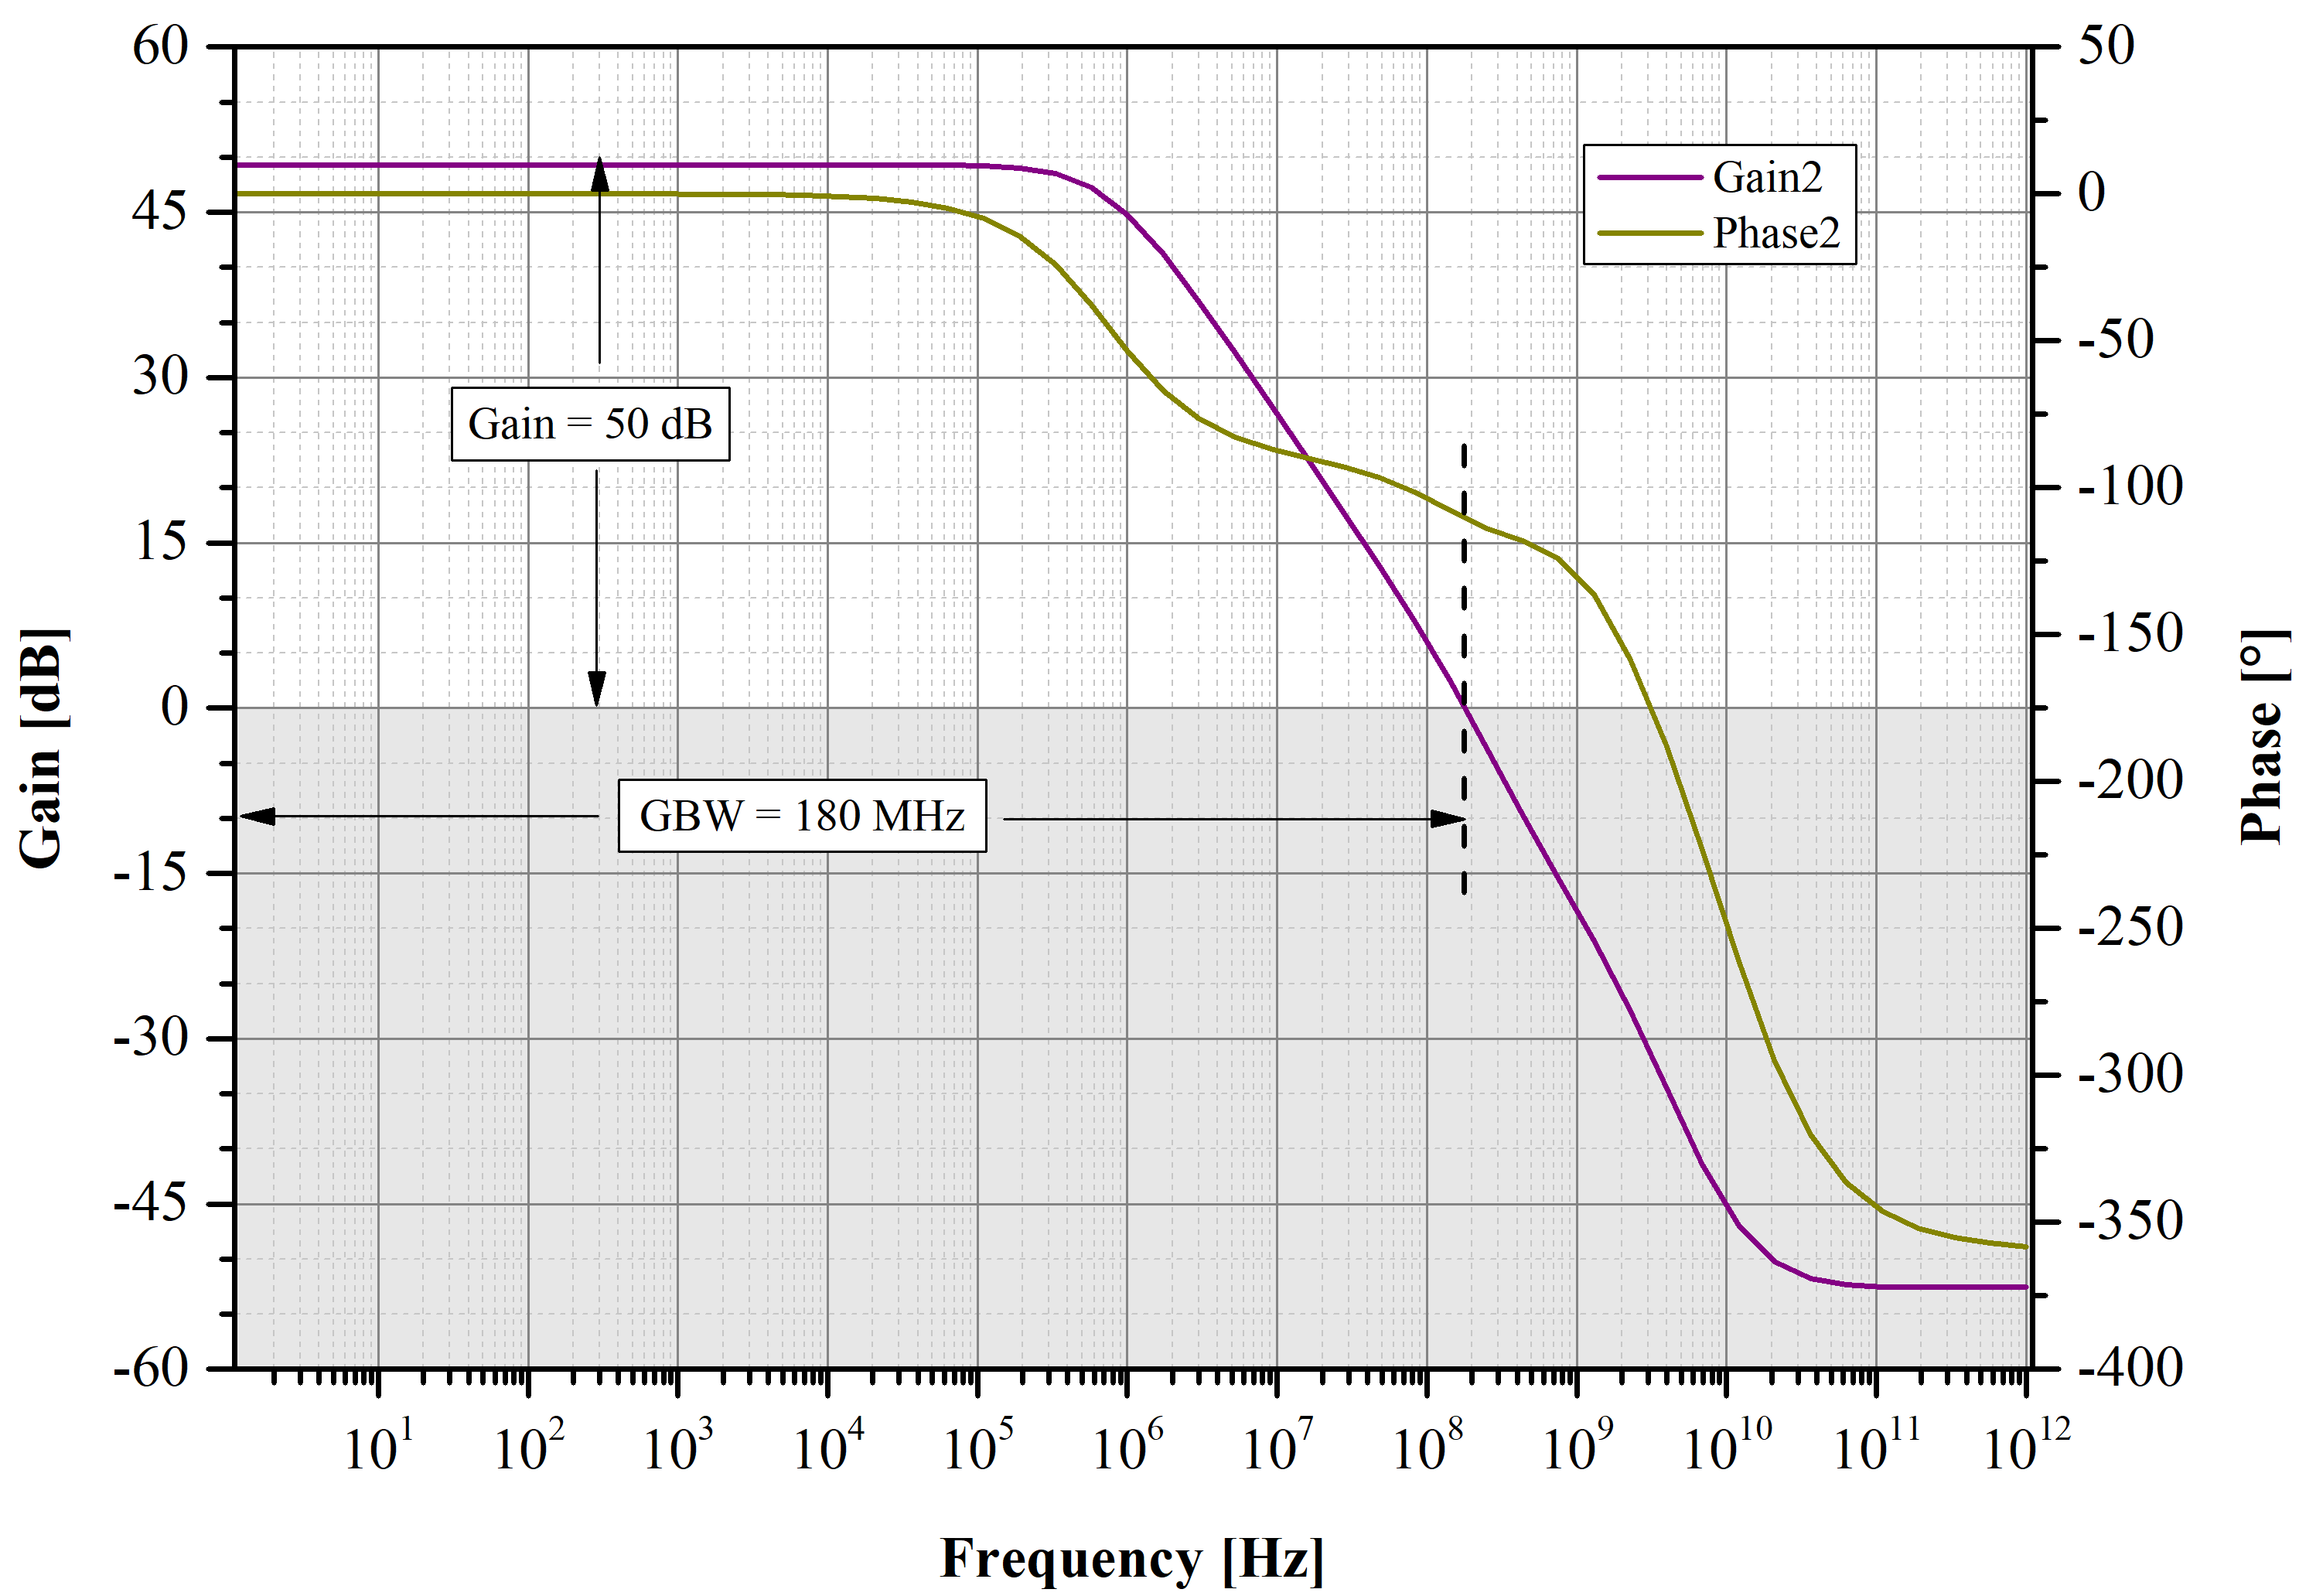
\includegraphics[width=0.85\columnwidth]{Chap05/Figures/gain2_phase2_vs_freq.png}
% \caption{Frequency Response of the Op-amp used in the Second integrator}
% \label{fig:gain2_phase2}
% \end{figure}
% %
\section{Quantizer}
A quantizer block in the IADC to be employed is of the resolution of 3-bit i.e. 8 levels as extracted from the simulink simulations. Therefore the total number of comparators needed to build a quantizer are $(2^{N_{SD}}-1)$ i.e. 7. Each comparator has a different threshold voltage where these thresholds are generated from the switched capacitor arrangement. 

\subsection{Threshold Generator}
The simplest solution to generate the thresholds of the comparator is a resistive ladder as shown in Fig.\ref{fig:res_lad}. The differential threshold is the difference of the voltage generated by resistive dividers at that node, e.g. the threshold $V_{1}$ can be given as,
%
\begin{equation}
    \begin{split}
        V_1 &= \frac{\left(\frac{9R}{2}\right)}{7R}\left(V_{refp}-V_{refn}\right)-\frac{\left(\frac{5R}{2}\right)}{7R}\left(V_{refp}-V_{refn}\right)\\
            &=\frac{4}{14}\left(V_{refp}-V_{refn}\right)
    \end{split}
\end{equation}
%
However, the resistors stacked between the positive and negative references tend to draw considerable amount of current, which then has to be taken into account while budgeting the power. The power consumption in the this threshold generator can be minimized by increasing the unit resistance value. 
%
\begin{figure}[h]
\centering
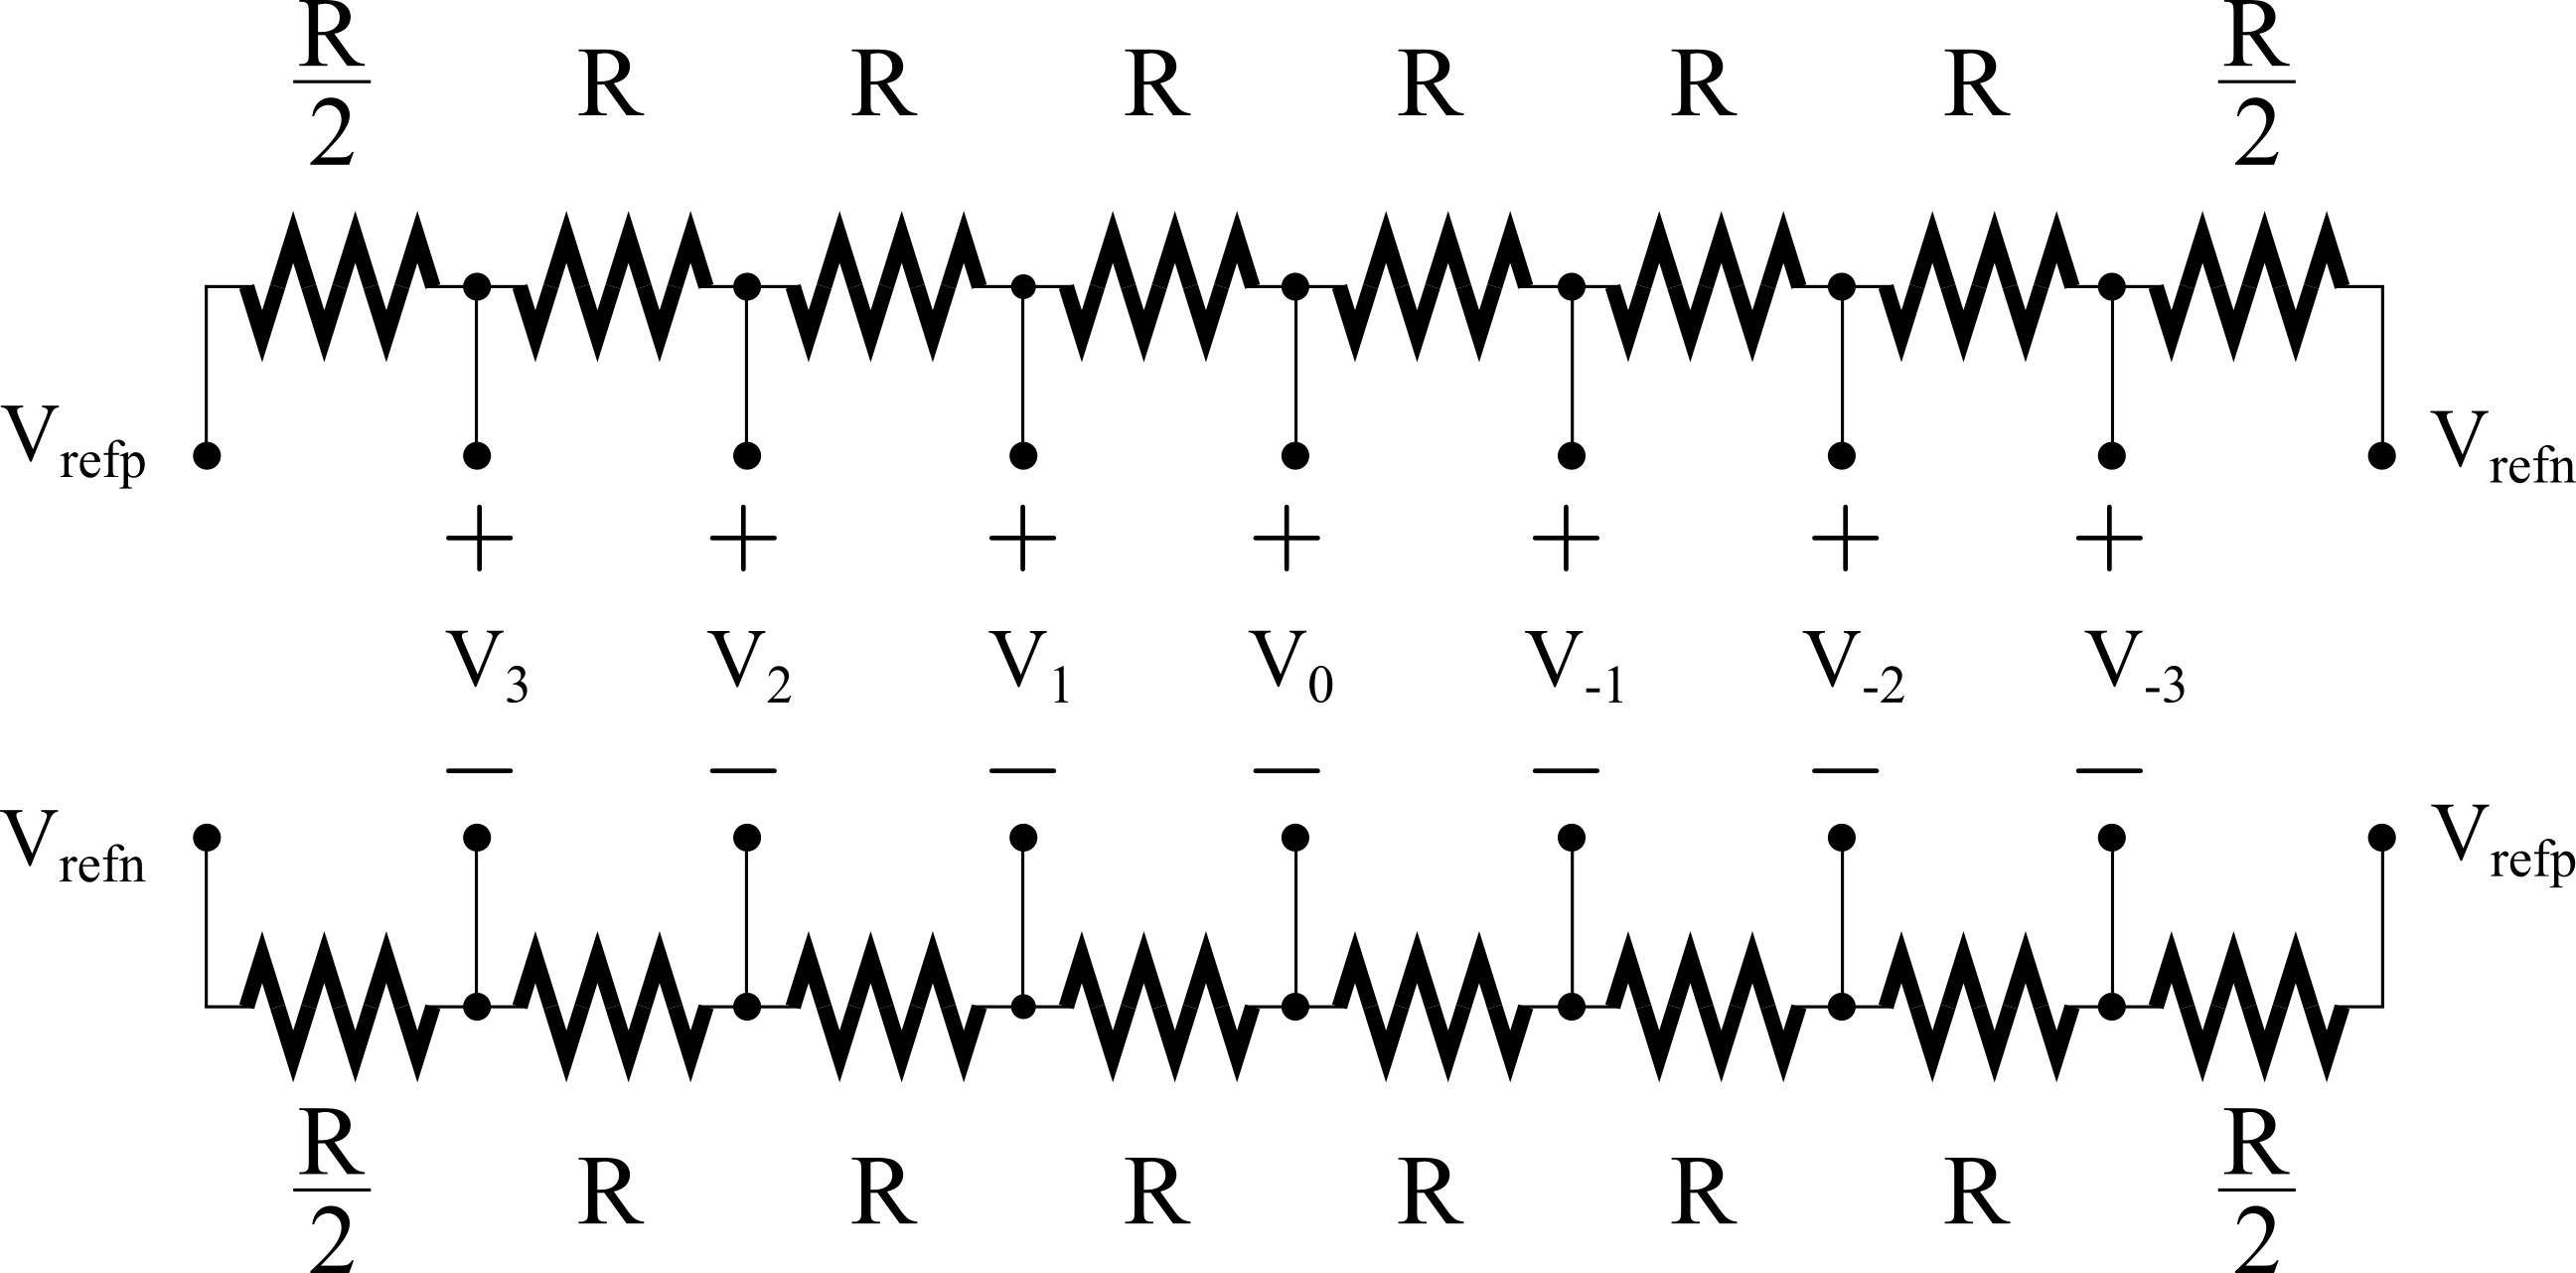
\includegraphics[width=0.85\columnwidth]{Chap05/Figures/resistive_ladder.png}
\caption{Resistive Ladder generating differential threshold voltages for comparators}
\label{fig:res_lad}
\end{figure}
%
But as it is known, the noise in the resistor is proportional to it's value, i.e. $V_{noise}^2=4kTR$, increase in the resistance in order to save the power would end up in noisy thresholds which will then corrupt the comparator decision causing degradation in the performance.

A switched-capacitor arrangement can be employed as an option to the resistive-ladder as shown in Fig. \ref{fig:switched_cap} which saves the static power consumption.
%
\begin{figure}[h!]
\centering
\subfigure[]{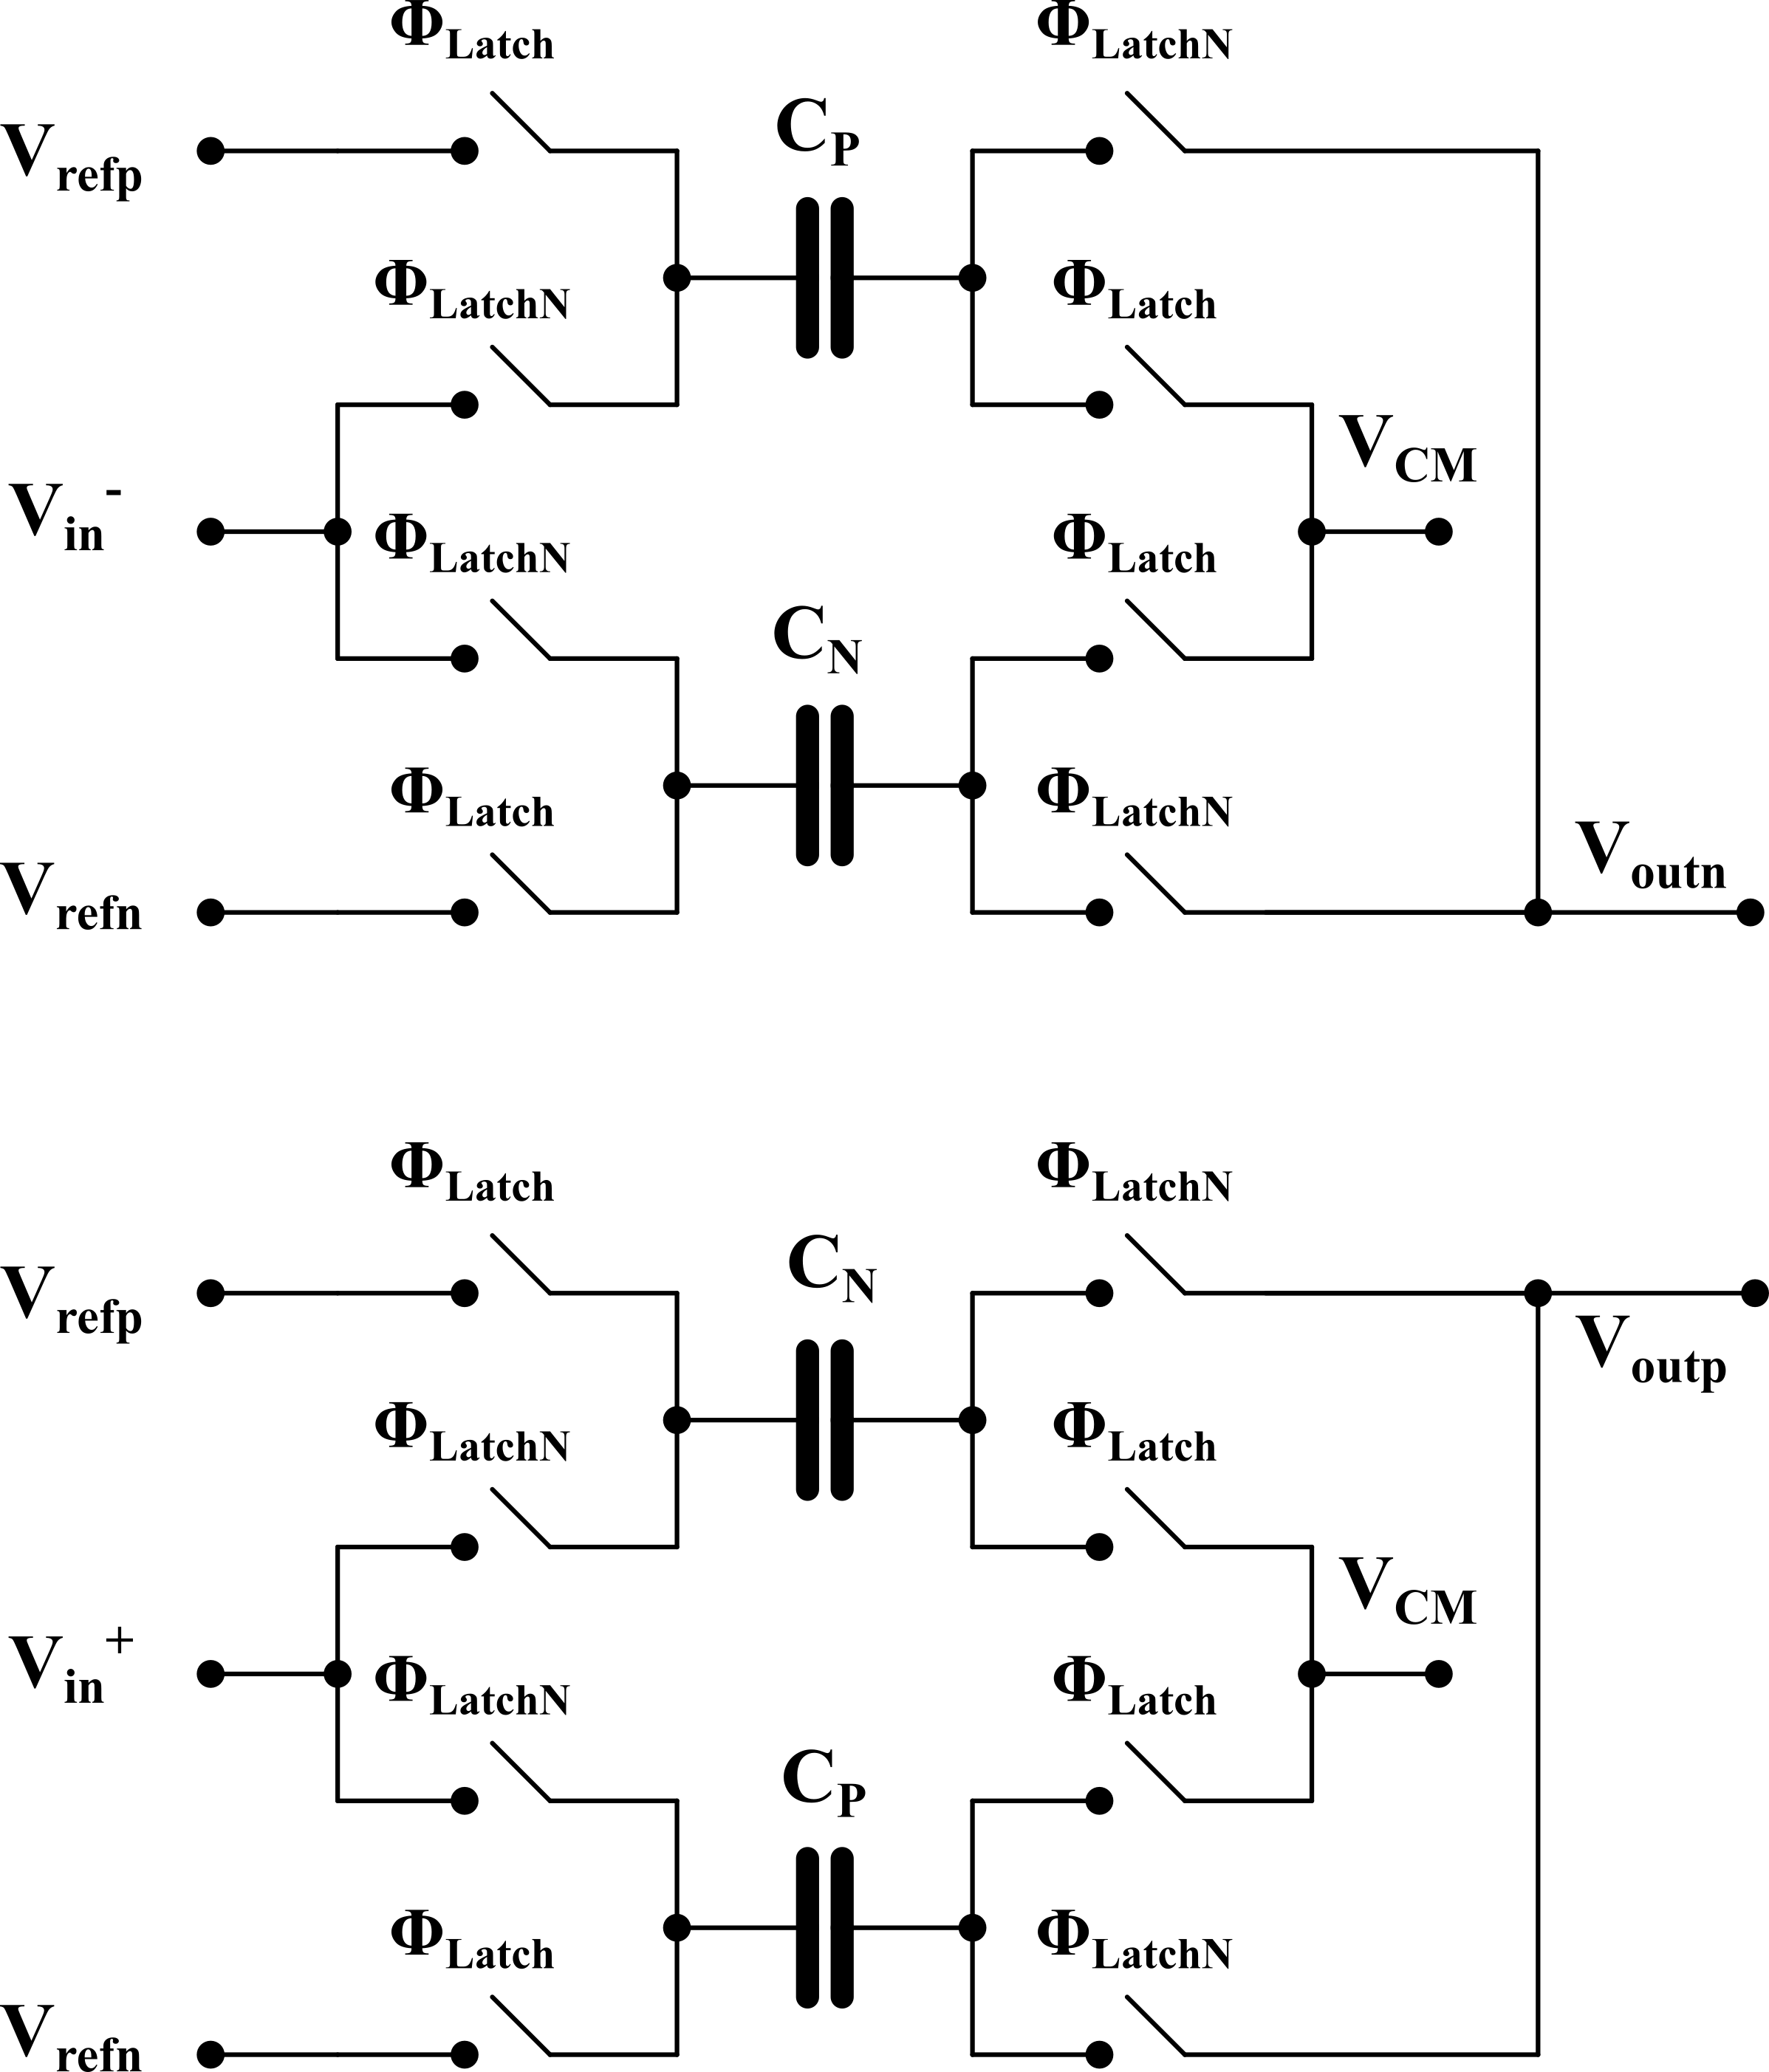
\includegraphics[scale=.32]{Chap05/Figures/switched_cap_thr.png}}\\
\qquad
\subfigure[]{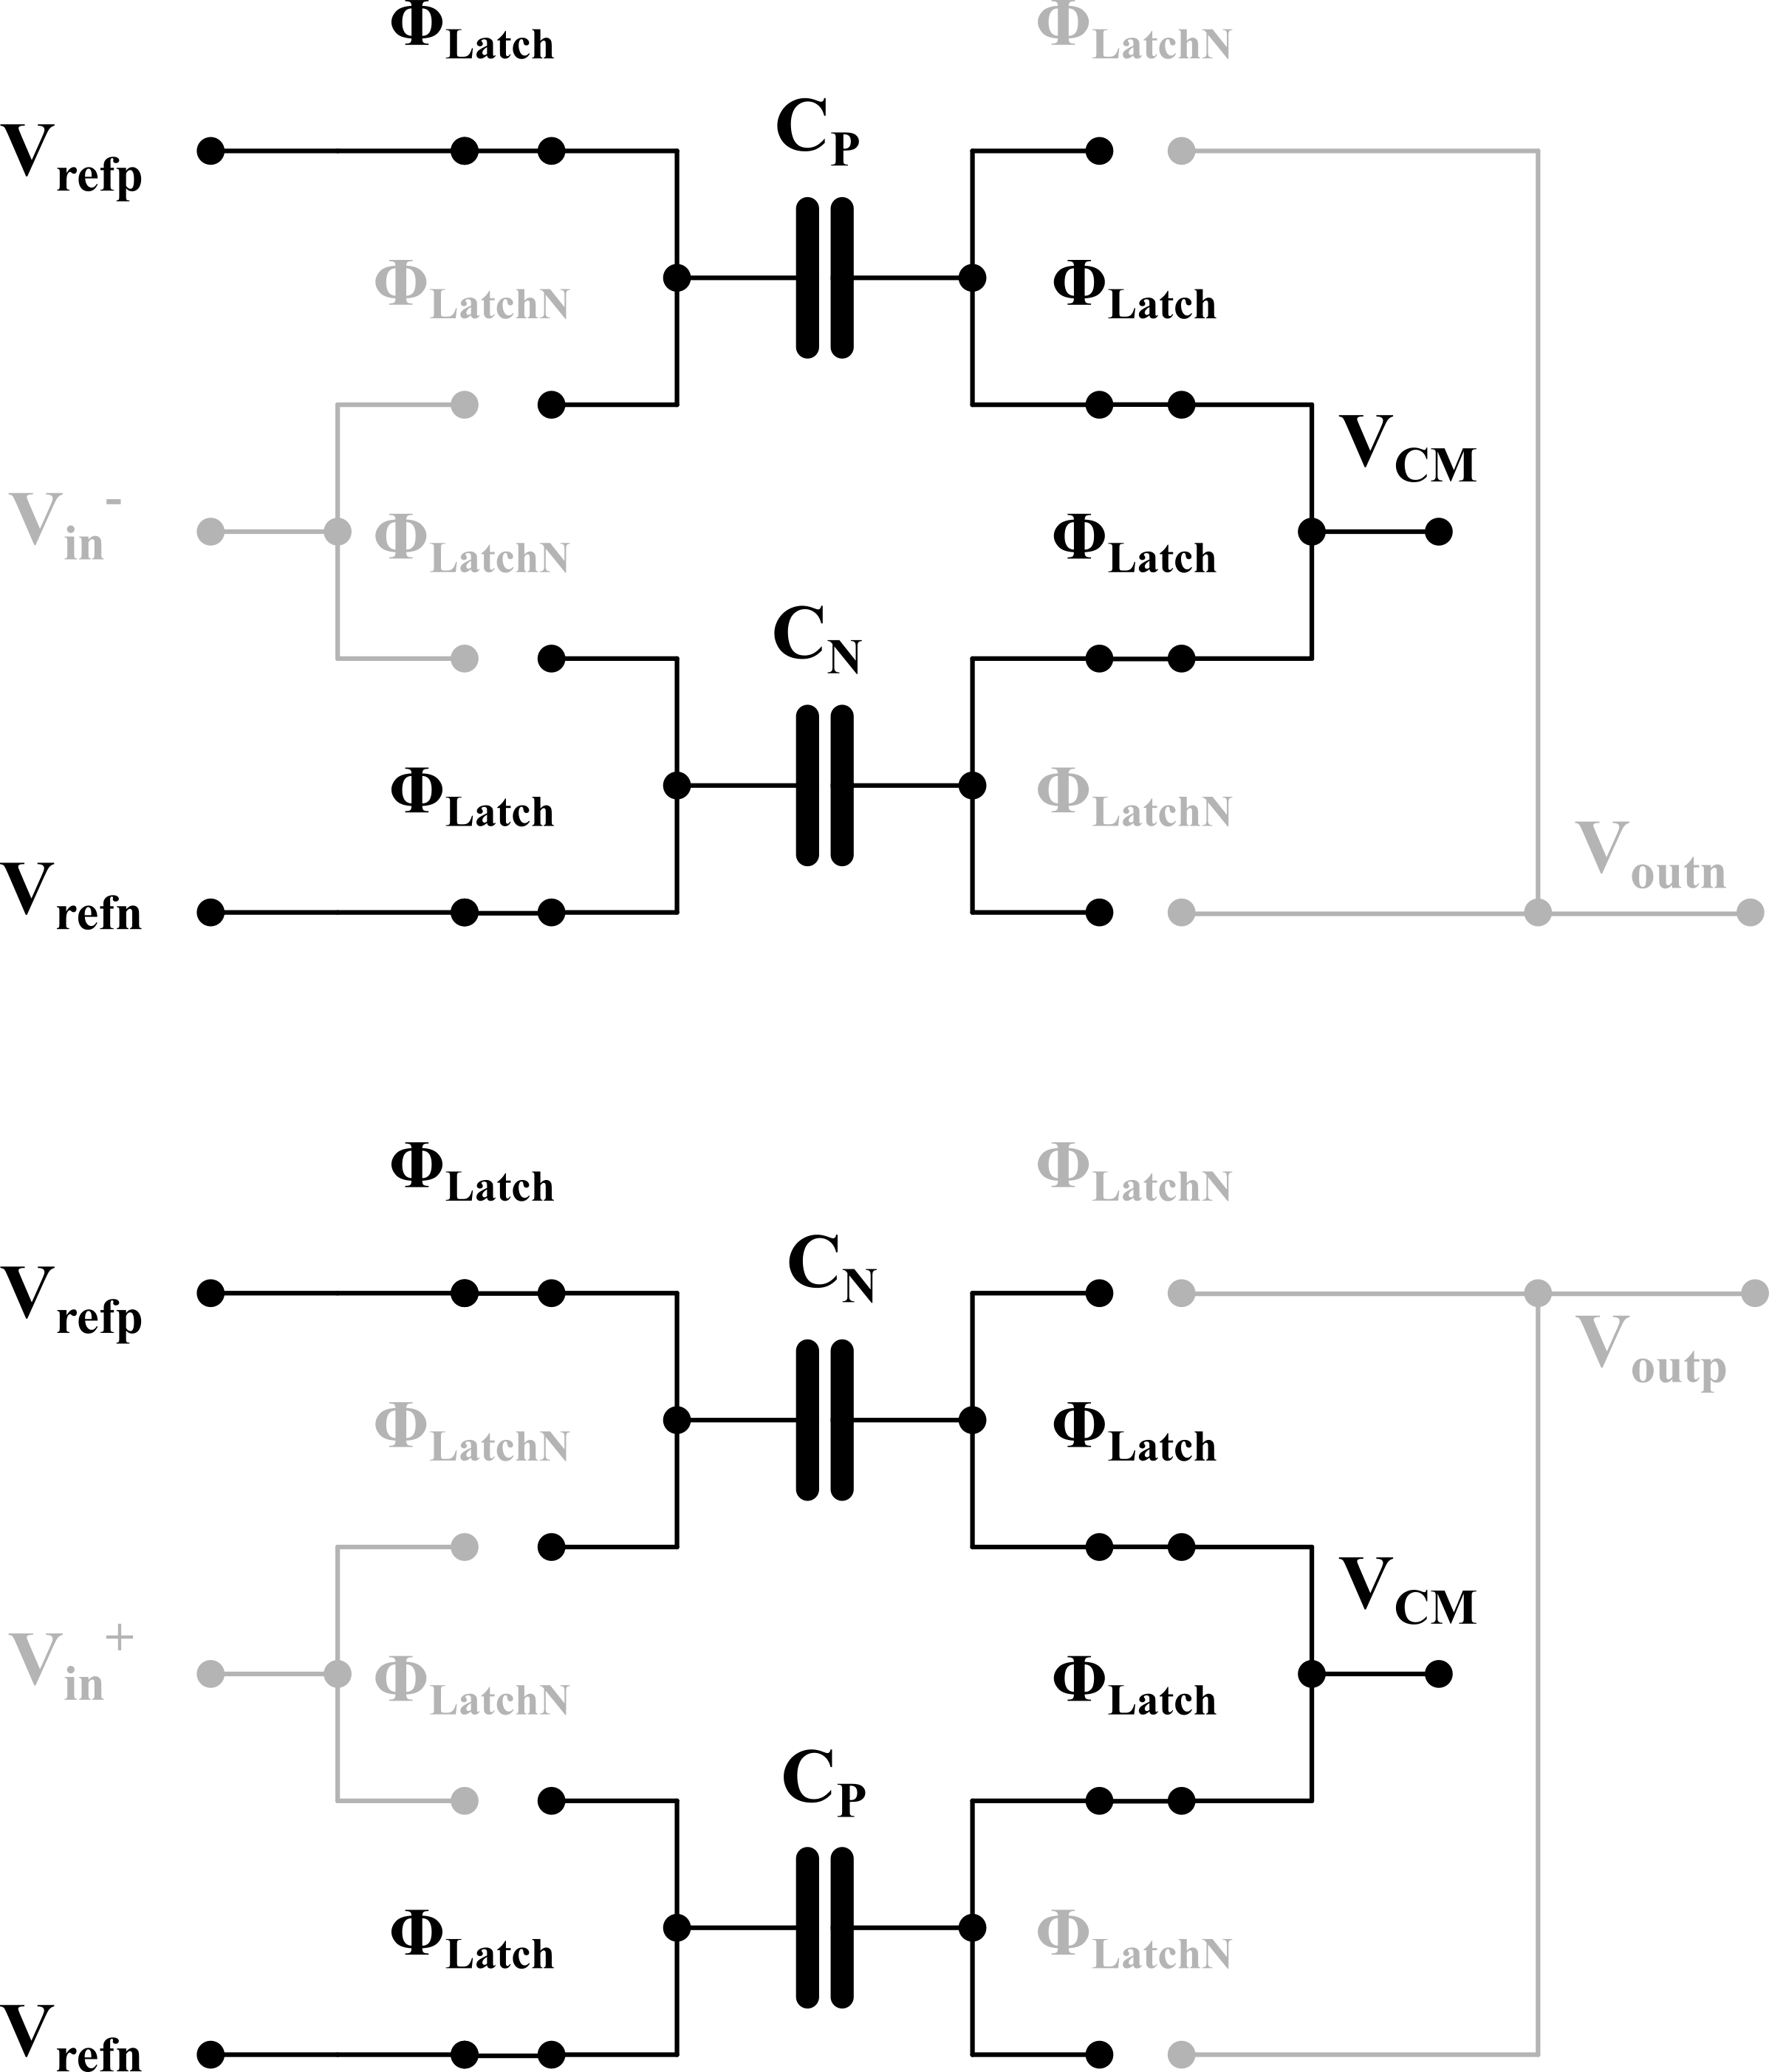
\includegraphics[scale=.32]{Chap05/Figures/switched_cap_thr_latch.png}}
\qquad
\subfigure[]{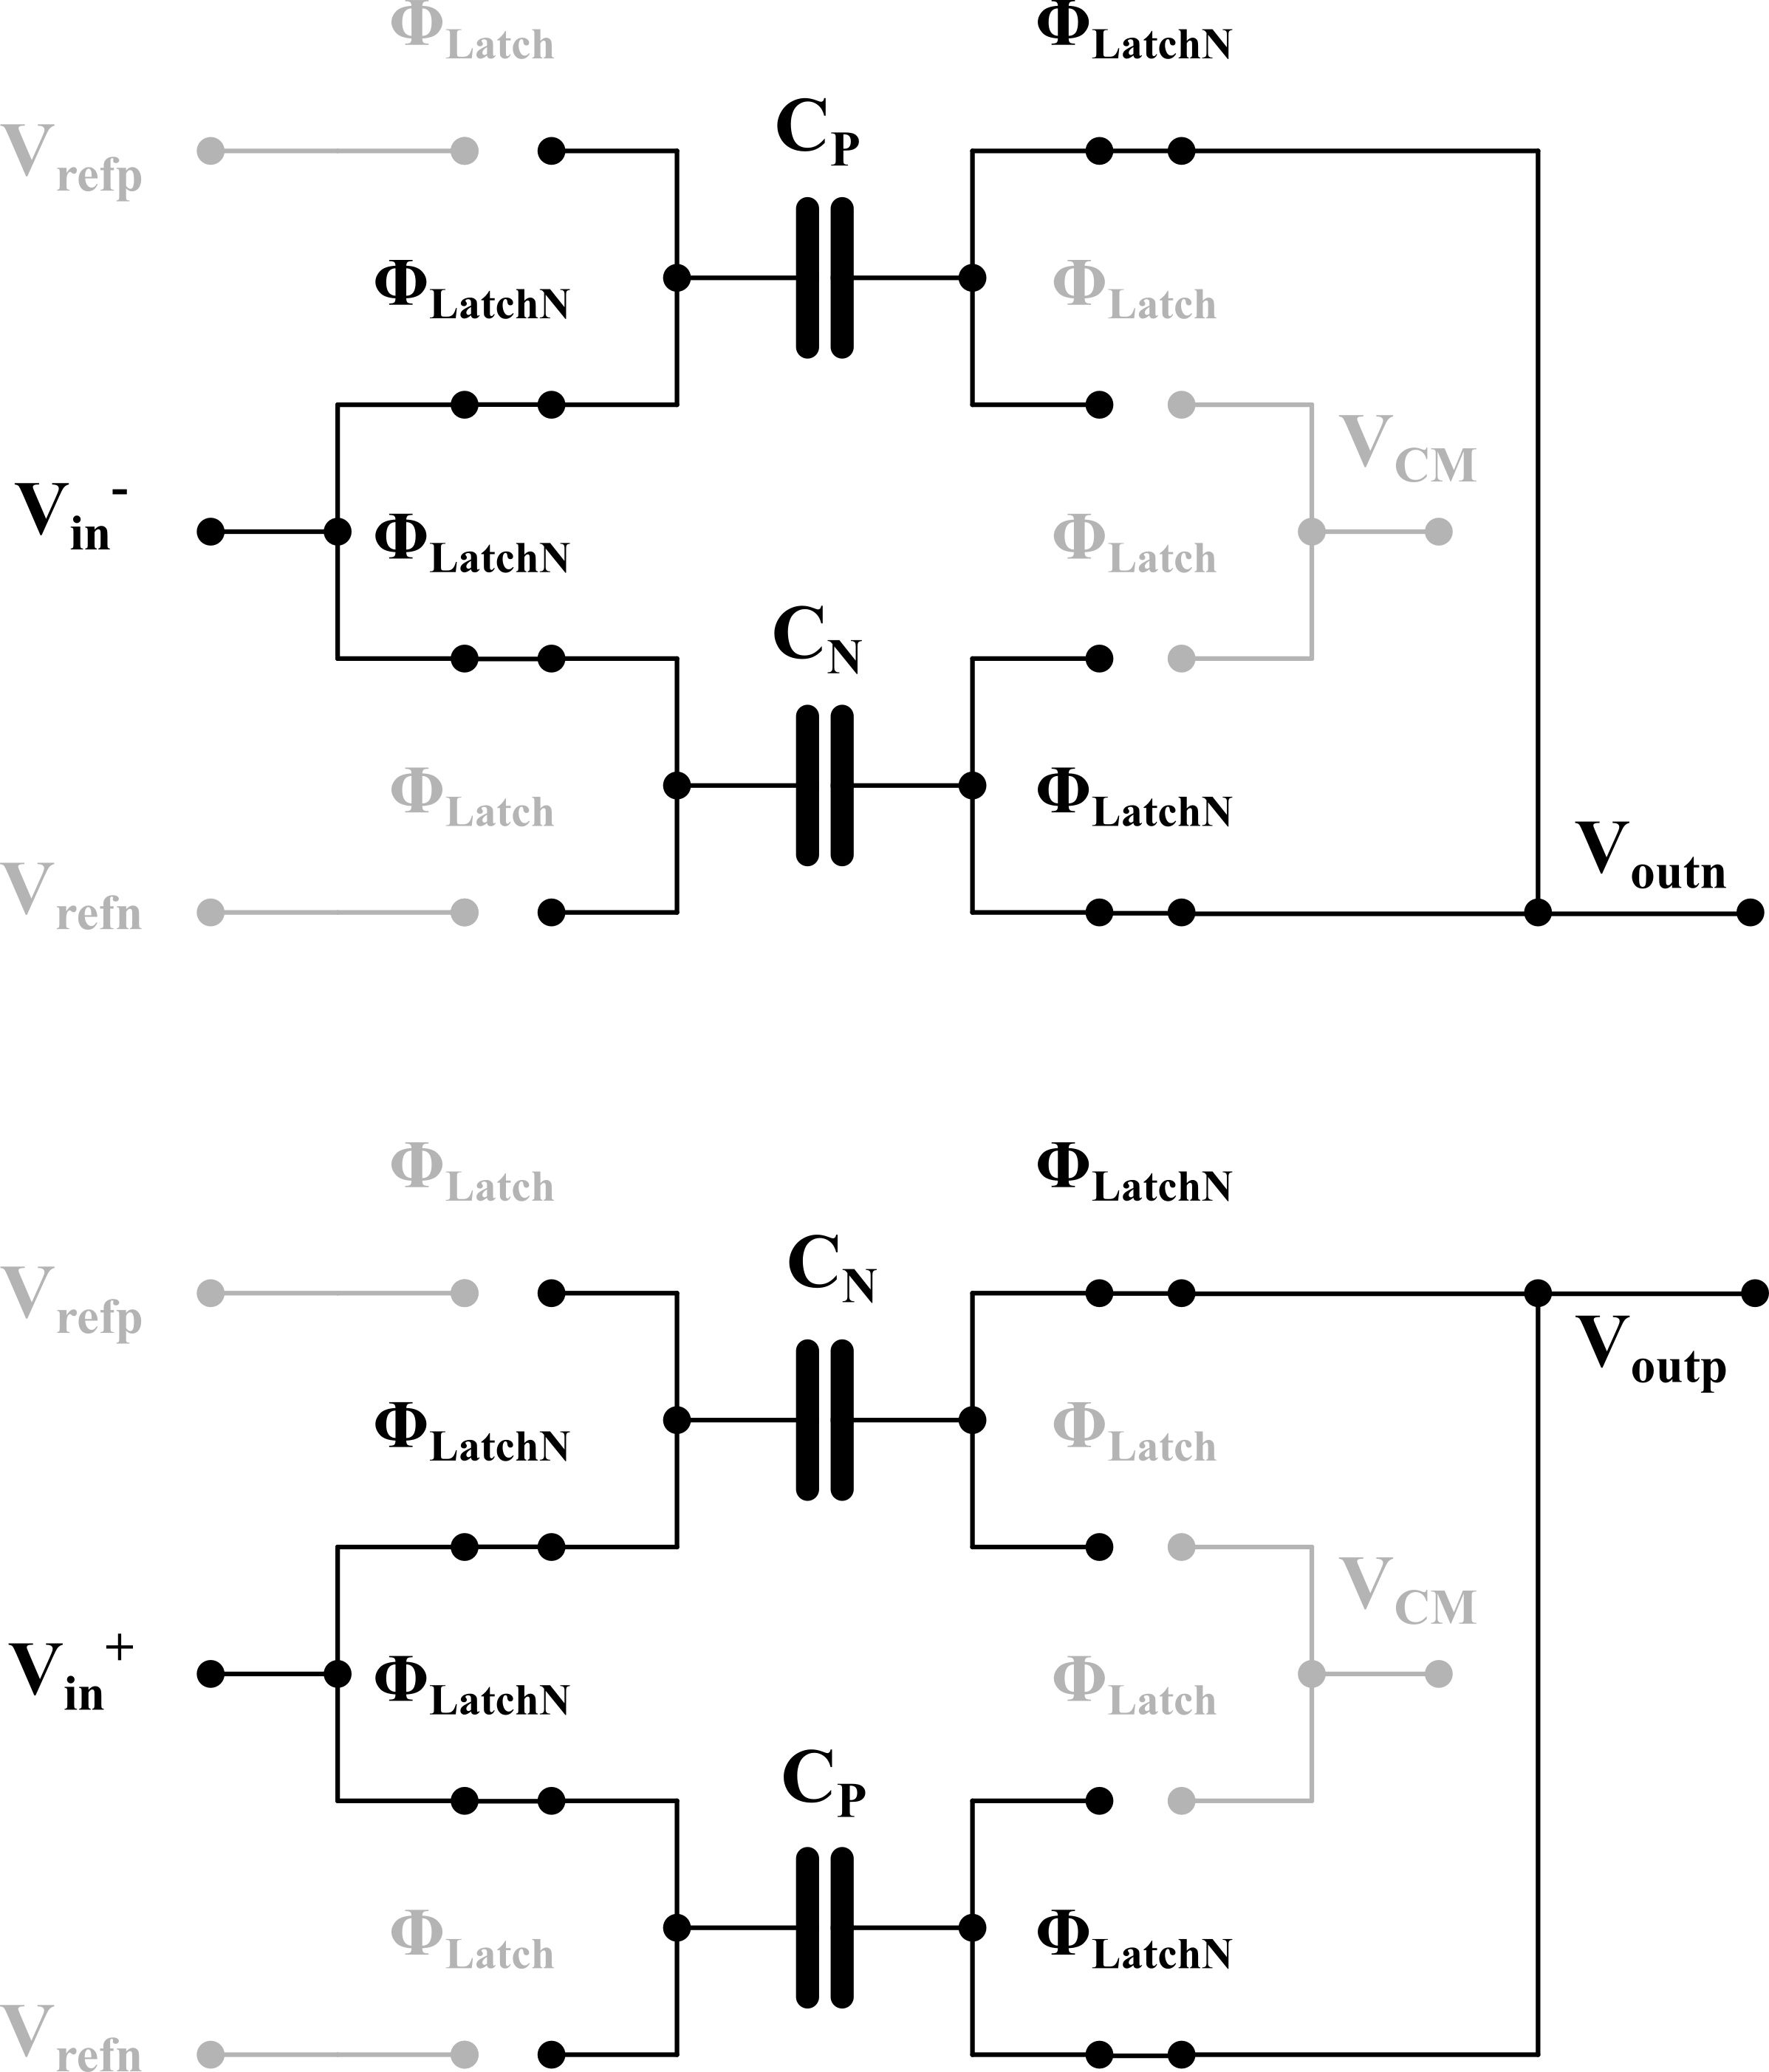
\includegraphics[scale=.32]{Chap05/Figures/switched_cap_thr_latchN.png}}
\caption{(a)Switched capacitor arrangement to generate threshold and taking difference with input sample (b)Threshold generator in a phase sampling reference voltage (c)Threshold generator in a phase sampling signal voltage}
\label{fig:switched_cap}
\end{figure}
%
In the Fig. \ref{fig:switched_cap}(a), the configuration of threshold generator is shown where the reference voltage is sampled on the capacitors with respect to the common mode voltage. Therefore, the charge stored on capacitors $C_{P_{U}}$, $C_{N_{U}}$, $C_{P_{L}}$ and $C_{N_{L}}$ are, ($C_{P_{U}}$=$C_{P_{L}}$=$C_P$, $C_{N_{U}}$=$C_{N_{L}}$=$C_N$)
%
\begin{equation}
    \begin{split}
        Q_{CP_{U}} &= C_{P_{U}}V_{refp} =C_PV_{refp}\\
        Q_{CN_{U}} &= C_{N_{U}}V_{refn} =C_NV_{refn}\\
        Q_{CP_{L}} &= C_{P_{L}}V_{refn} =C_PV_{refn}\\
        Q_{CN_{L}} &= C_{N_{L}}V_{refp} =C_NV_{refp}
    \end{split}
\end{equation}
%
In the next phase where the input signal is sampled, the capacitors $C_{P_{U}}$ and $C_{N_{U}}$ are in parallel which makes it $C_U=C_{P_{U}}+C_{N_{U}}$. Similarly, $C_{P_{L}}$ and $C_{N_{L}}$ parallel combination exhibit the total equivalent capacitance of $C_L=C_{P_{L}}+C_{N_{L}}$. Then the charge and voltage across the capacitors $C_U$ and $C_L$ can be given by,
%
\begin{equation}
    \begin{split}
        Q_{CU} &= Q_{CP_{U}}+Q_{CN_{U}}\\
        (C_P+C_N)V_{CU} &= C_PV_{refp}+C_NV_{refn}
    \end{split}
\end{equation}
%
%
\begin{equation}
        V_{CU}=\frac{C_PV_{refp}+C_NV_{refn}}{C_P+C_N}
\end{equation}
%
similarly,
%
\begin{equation}
        V_{CL}=\frac{C_PV_{refn}+C_NV_{refp}}{C_P+C_N}
\end{equation}
%
Then the voltage difference of $V_{outp}$ and $V_{outn}$ can be expressed as,
%
\begin{equation}
    \begin{split}
        V_{out} &= V_{outp}-V_{outn}\\
                &= (V_{in}^--V_{CU})-(V_{in}^+-V_{CL})\\
                &= \left(V_{in}^--\frac{C_PV_{refp}+C_NV_{refn}}{C_P+C_N}\right)-\left(V_{in}^+-\frac{C_PV_{refn}+C_NV_{refp}}{C_P+C_N}\right)\\
                &= \left(V_{in}^+-V_{in}^-\right)-\frac{C_P-C_N}{C_P+C_N}\left(V_{refp}-V_{refn}\right)\\
                &= V_{in}-V_{thr}
    \end{split}
\end{equation}
%
where the threshold voltage generated by the switched capacitor is,
%
\begin{equation}\label{THR_GEN}
    V_{thr} = \frac{C_P-C_N}{C_P+C_N}\left(V_{refp}-V_{refn}\right)
\end{equation}
%
and, $V_{ref}= V_{refp} - V_{refn}$. 

For multi-bit quantizer, the different values of $C_P$ and $C_N$ generates the different values of the threshold voltages while the total capacitance $C_P+C_N$ is equal. The following table shows the different values of the threshold voltages created by the switched-capacitor block shown in Fig. \ref{fig:switched_cap}, for 3-bit quantizer.
\begin{table}[h!]
\centering
\begin{tabular}{c|c|c}
\Xhline{4\arrayrulewidth}
\textbf{C\textsubscript{P}}      & \textbf{C\textsubscript{N}}      & \textbf{V\textsubscript{thr}} (Volts)     \\ \hline
350 fF                             & 50  fF                             & (3/4)V\textsubscript{ref} \\ \hline
300 fF                             & 100 fF                             & (2/4)V\textsubscript{ref} \\ \hline
250 fF                             & 150 fF                             & (1/4)V\textsubscript{ref} \\ \hline
200 fF                             & 200 fF                             & (0/4)V\textsubscript{ref} \\ \hline
150 fF                             & 250 fF                             & -(1/4)V\textsubscript{ref} \\ \hline
100 fF                             & 300 fF                             & -(2/4)V\textsubscript{ref} \\ \hline
50  fF                             & 350 fF                             & -(3/4)V\textsubscript{ref} \\ \Xhline{4\arrayrulewidth}
\end{tabular}
\caption{The threshold voltages generated for 3-bit quantizer}
\label{tab:vthr}
\end{table}

However, since the signal swing at the output of second integrator is reduced 4 times, which is the input to the quantizer, the signal do not cover full range of the quantizer but just $1/4^{th}$ part of the full-scale. This will result in the decreased SQNR as a consequence. In order for input signal to quantizer to cover the full-scale, now, solution is to scale the quantizer thresholds down by equal amount as the signal, i.e. by a factor of 4. The ratios of the capacitors in the threshold generator has to be modified as follows considering the unit capacitance of $C_{unit}=12.5~fF$ which still accounts the total capacitance $C_P~+~C_N~=~400~fF$ 
%
\begin{table}[h!]
\centering
\begin{tabular}{l|l|r}
\Xhline{4\arrayrulewidth}
\multicolumn{1}{c|}{\textbf{C\textsubscript{P}}}        & \multicolumn{1}{c|}{\textbf{C\textsubscript{N}}}     & \multicolumn{1}{c}{\textbf{V\textsubscript{thr}}}       \\ \hline
19C\textsubscript{unit} = 237.5 fF & 13C\textsubscript{unit} = 162.5 fF & (3/16)V\textsubscript{ref}  \\ \hline
18C\textsubscript{unit} = 225 fF      & 14C\textsubscript{unit} = 175 fF   & (2/16)V\textsubscript{ref}  \\ \hline
17C\textsubscript{unit} = 212.5 fF    & 15C\textsubscript{unit} = 187.5 fF & (1/16)V\textsubscript{ref}  \\ \hline
16C\textsubscript{unit} = 200 fF      & 16C\textsubscript{unit} = 200 fF   & (0/16)V\textsubscript{ref}  \\ \hline
15C\textsubscript{unit} = 187.5 fF    & 17C\textsubscript{unit} = 212.5 fF & -(1/16)V\textsubscript{ref} \\ \hline
14C\textsubscript{unit} = 175 fF      & 18C\textsubscript{unit} = 225 fF   & -(2/16)V\textsubscript{ref} \\ \hline
13C\textsubscript{unit} = 162.5 fF    & 19C\textsubscript{unit} = 237.5 fF & -(3/16)V\textsubscript{ref} \\ \Xhline{4\arrayrulewidth}
\end{tabular}
\caption{Modified threshold voltages, generated for 3-bit quantizer accommodating the signal to full scale.}
\label{tab:vthr_mod}
\end{table}
%
\subsection{Comparator}
The architecture of the comparator used in the quantizer is as shown in the Fig. \ref{COMP} which is designed to work with a clock frequency of $80\ MHz$. The driving transistors pair $M_{0}$ and $M_{1}$, constitutes a preamplifier. It amplifies the signal prior to the comparison and transmits it to the back-to-back connected NOT gate.
\begin{figure}[h!]
\centering
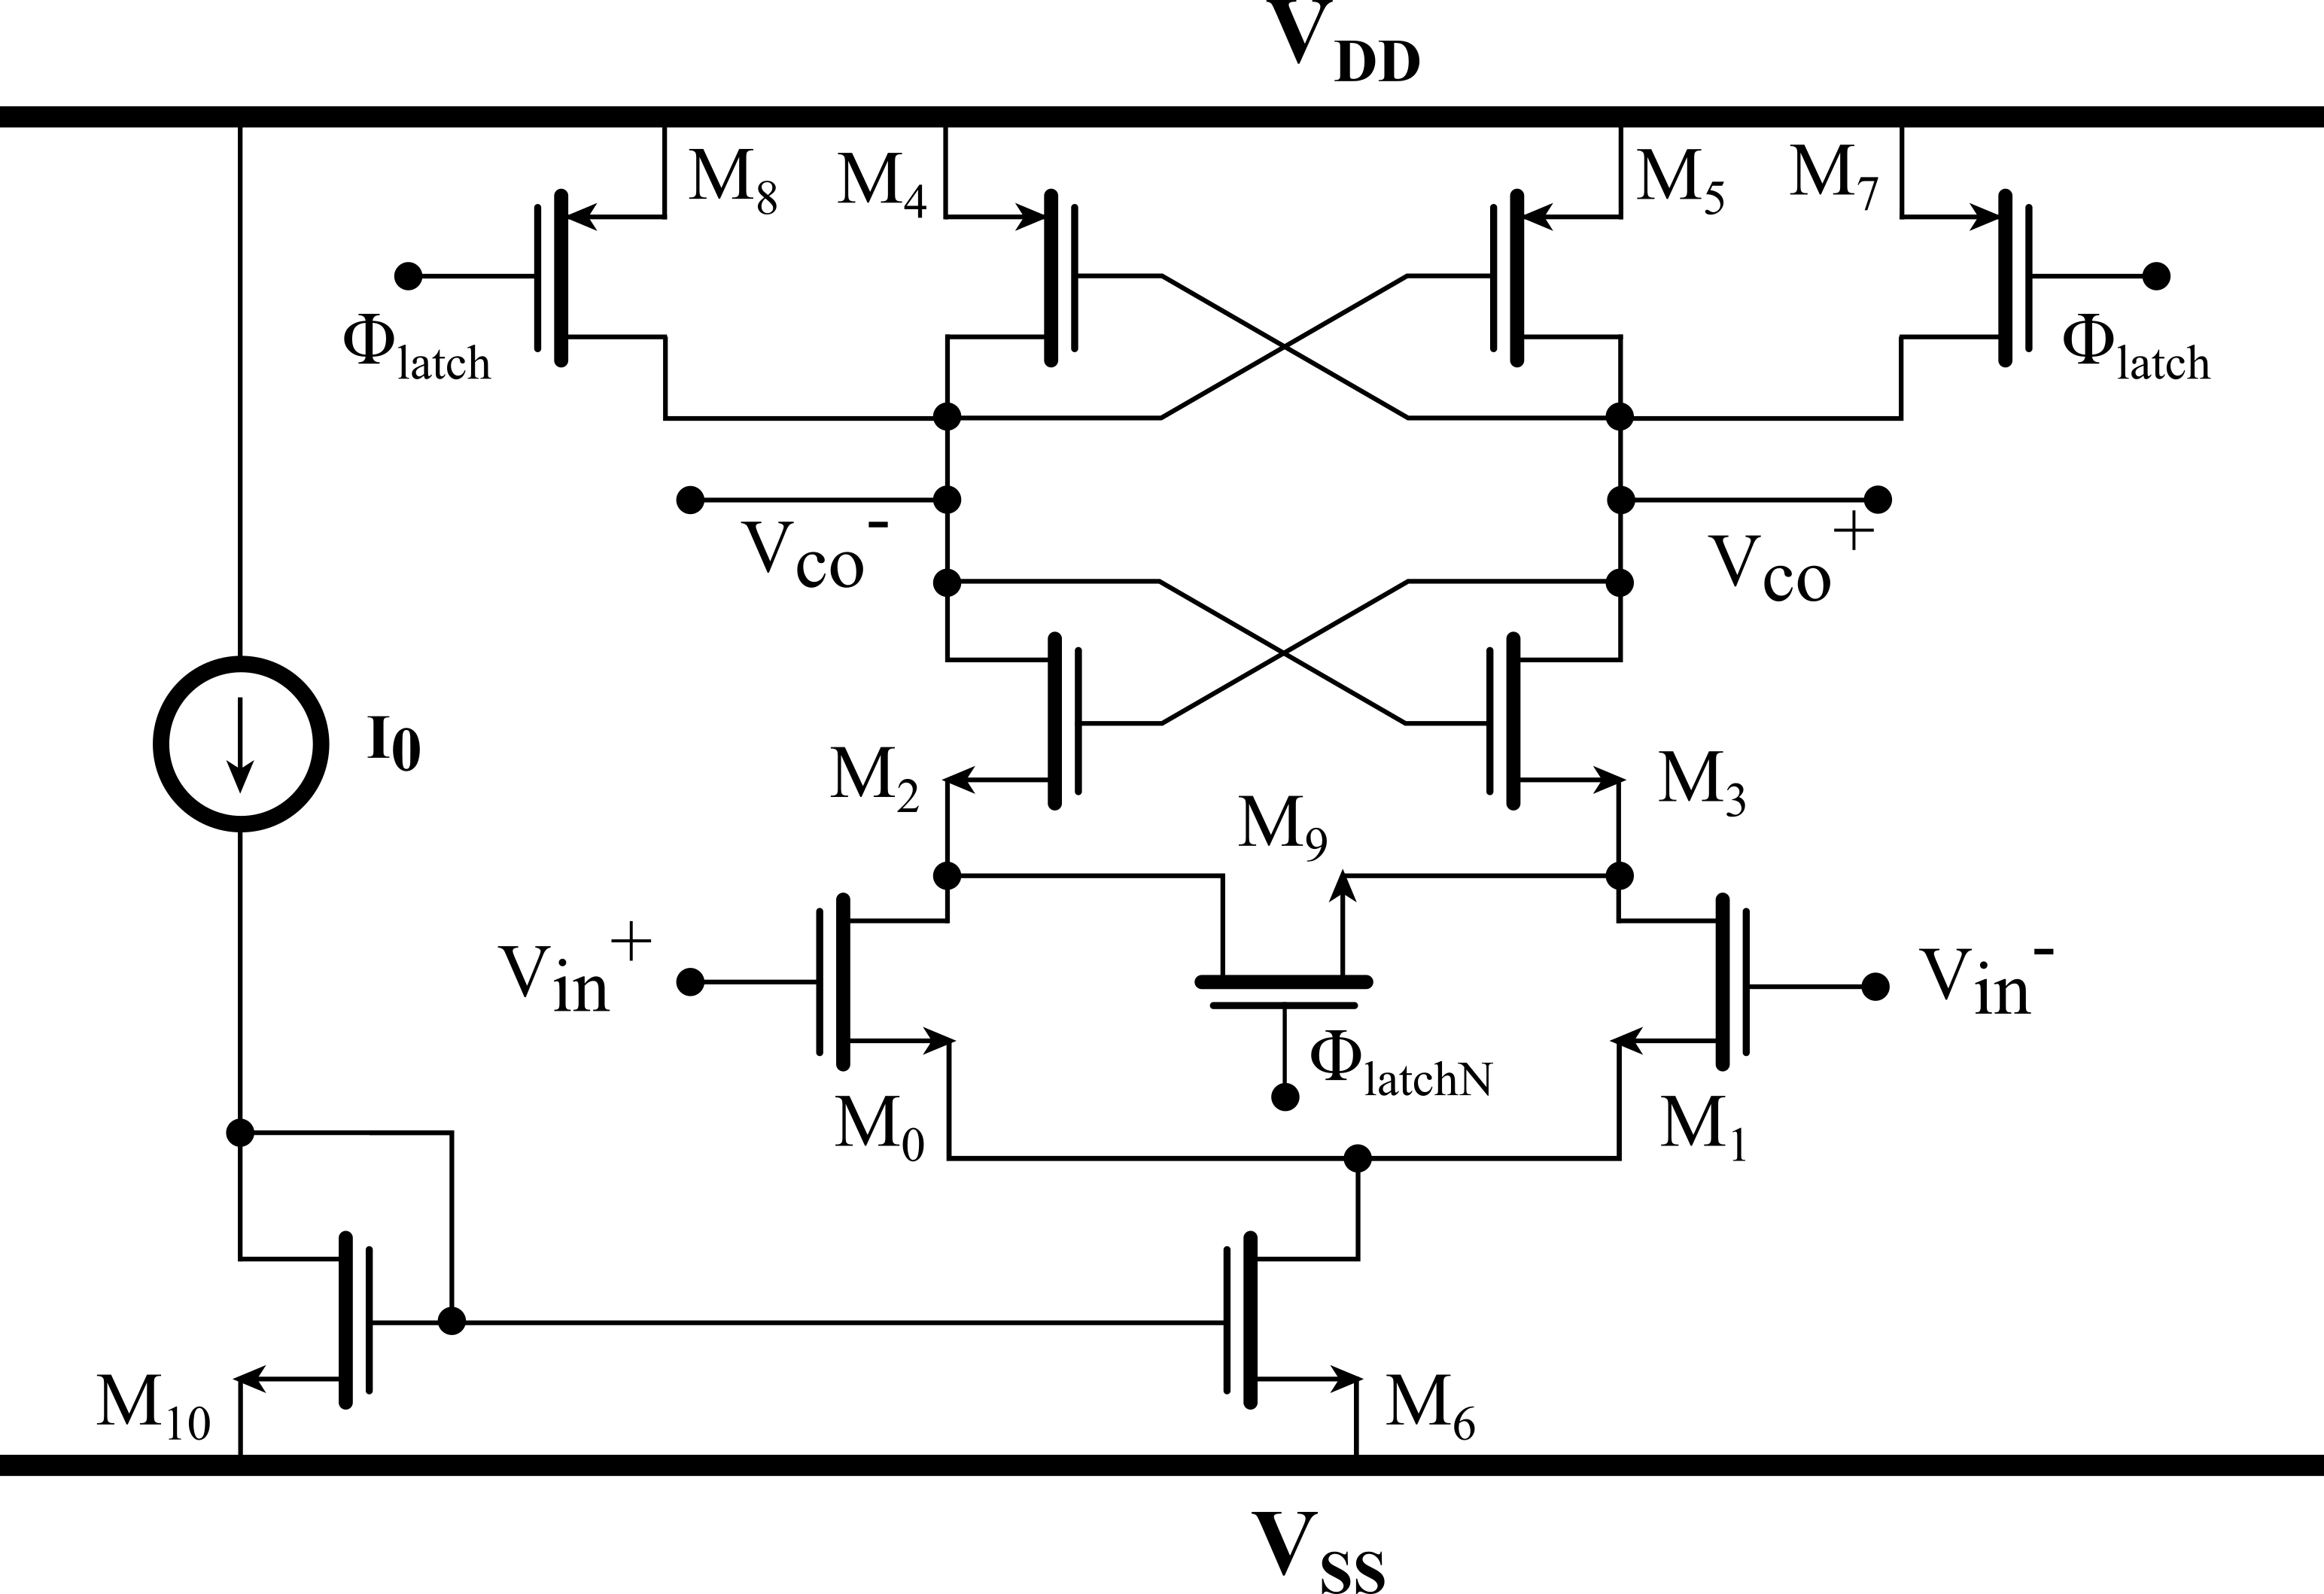
\includegraphics[width=0.8\columnwidth]{Chap05/Figures/comparator.png}
\caption{Schematic of the Comparator employed in the Quantizer}
\label{COMP}
\end{figure}
 This is a positive feedback circuit which pulls up or down the output node ($V_{CO}^+$ and $V_{CO}^-$) voltage depending on the signal transferred from the preamplifier and takes the decision.
These comparison signals can then be stored in the latch comprised of NAND gates and then are passed through the buffers to make the signals strong enough to drive the given load as shown in the Fig. \ref{LATCH}.
\begin{figure}[h!]
\centering
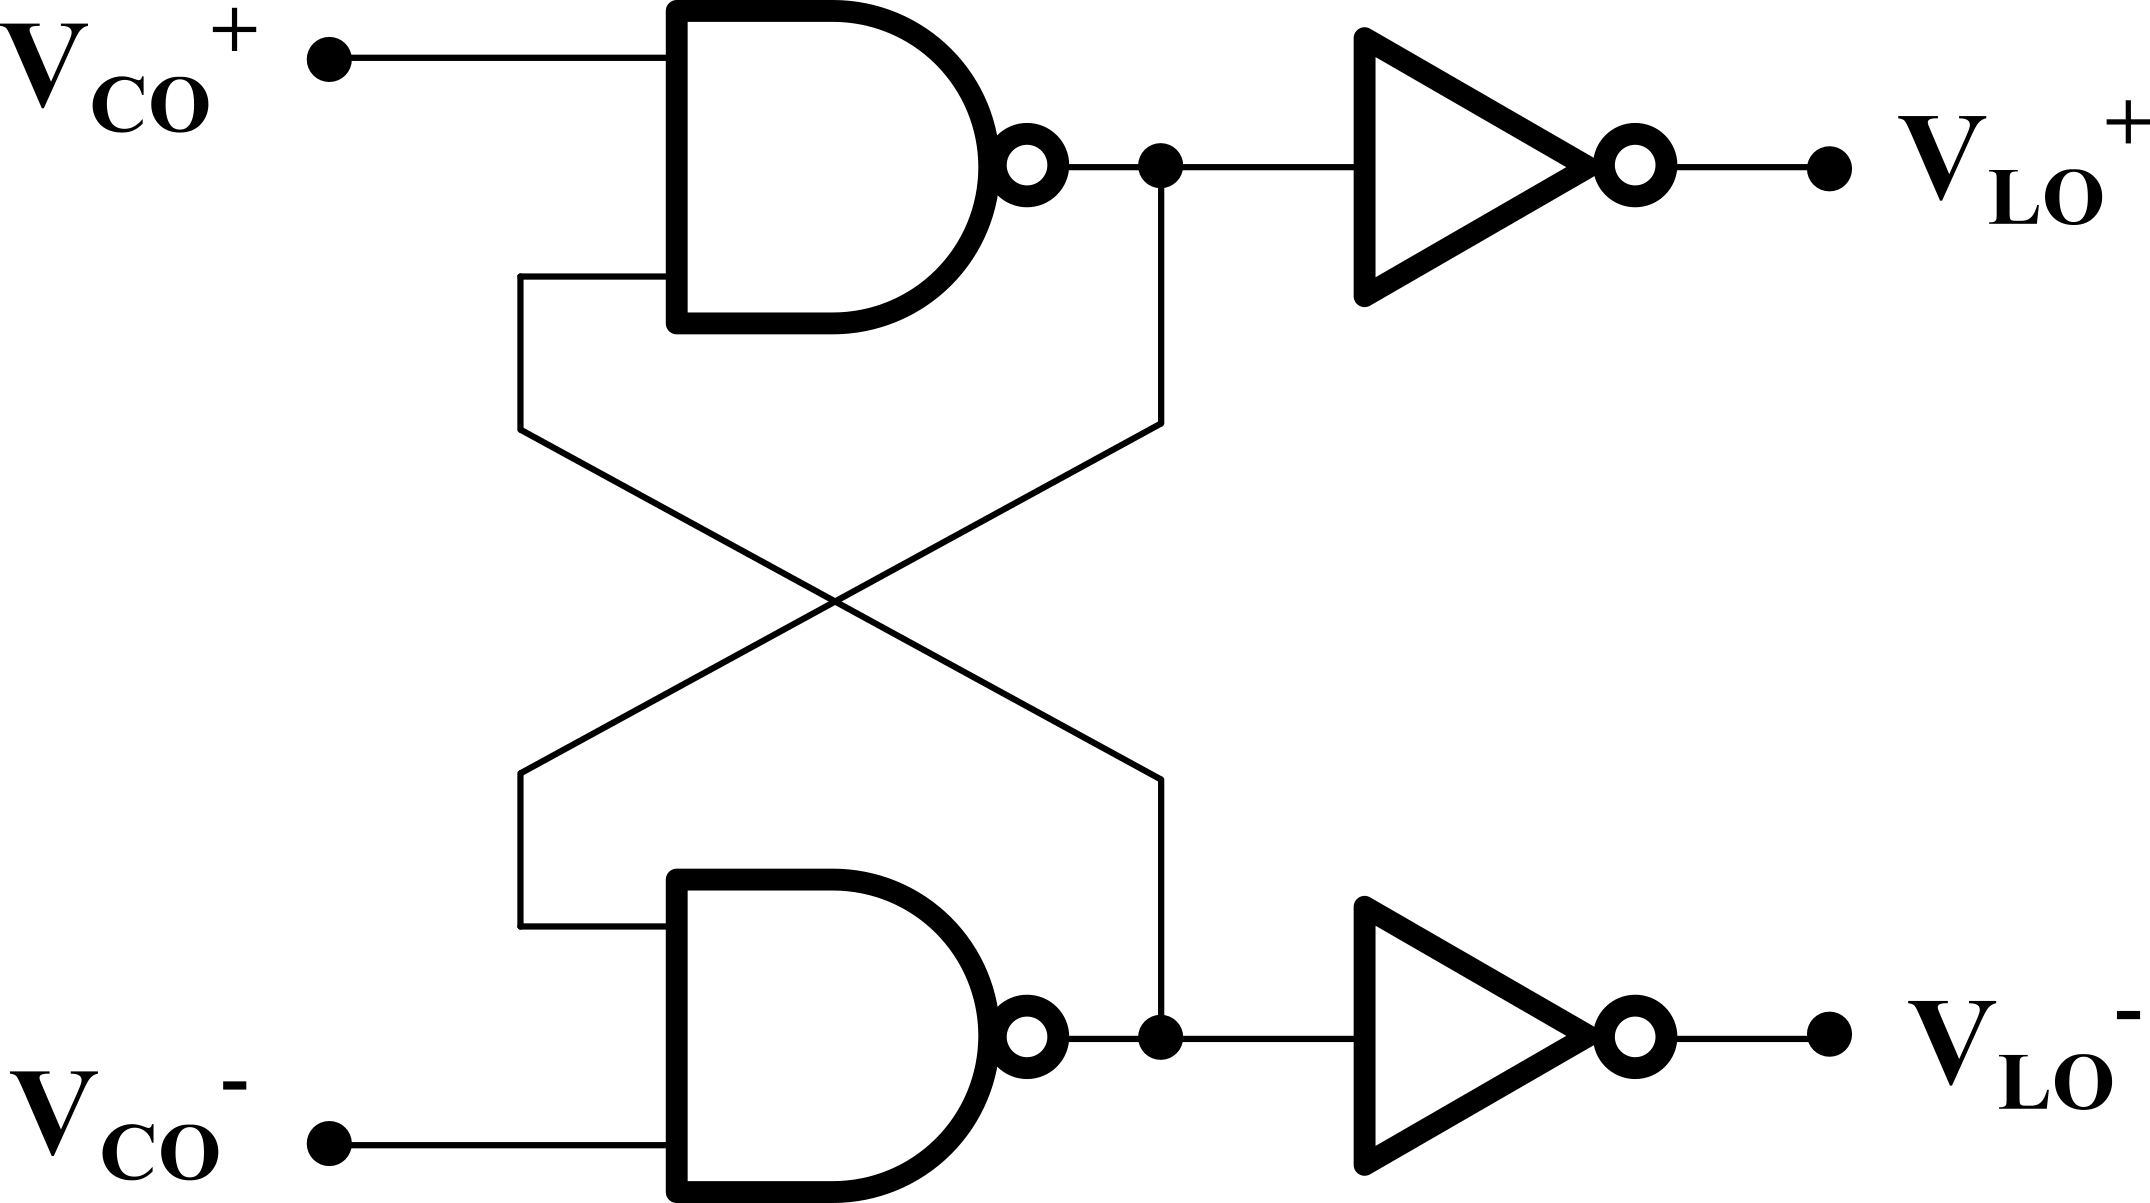
\includegraphics[width=0.5\columnwidth]{Chap05/Figures/latch.png}
\caption{Latch Comprised of NAND gates and digital buffers}
\label{LATCH}
\end{figure}
The capacitive divider is used to generate the threshold, specific for a comparator and it's value depends on the ratio of the capacitors, can be expressed as in the Eq. \ref{THR_GEN}.
\begin{figure}[h!]
\centering
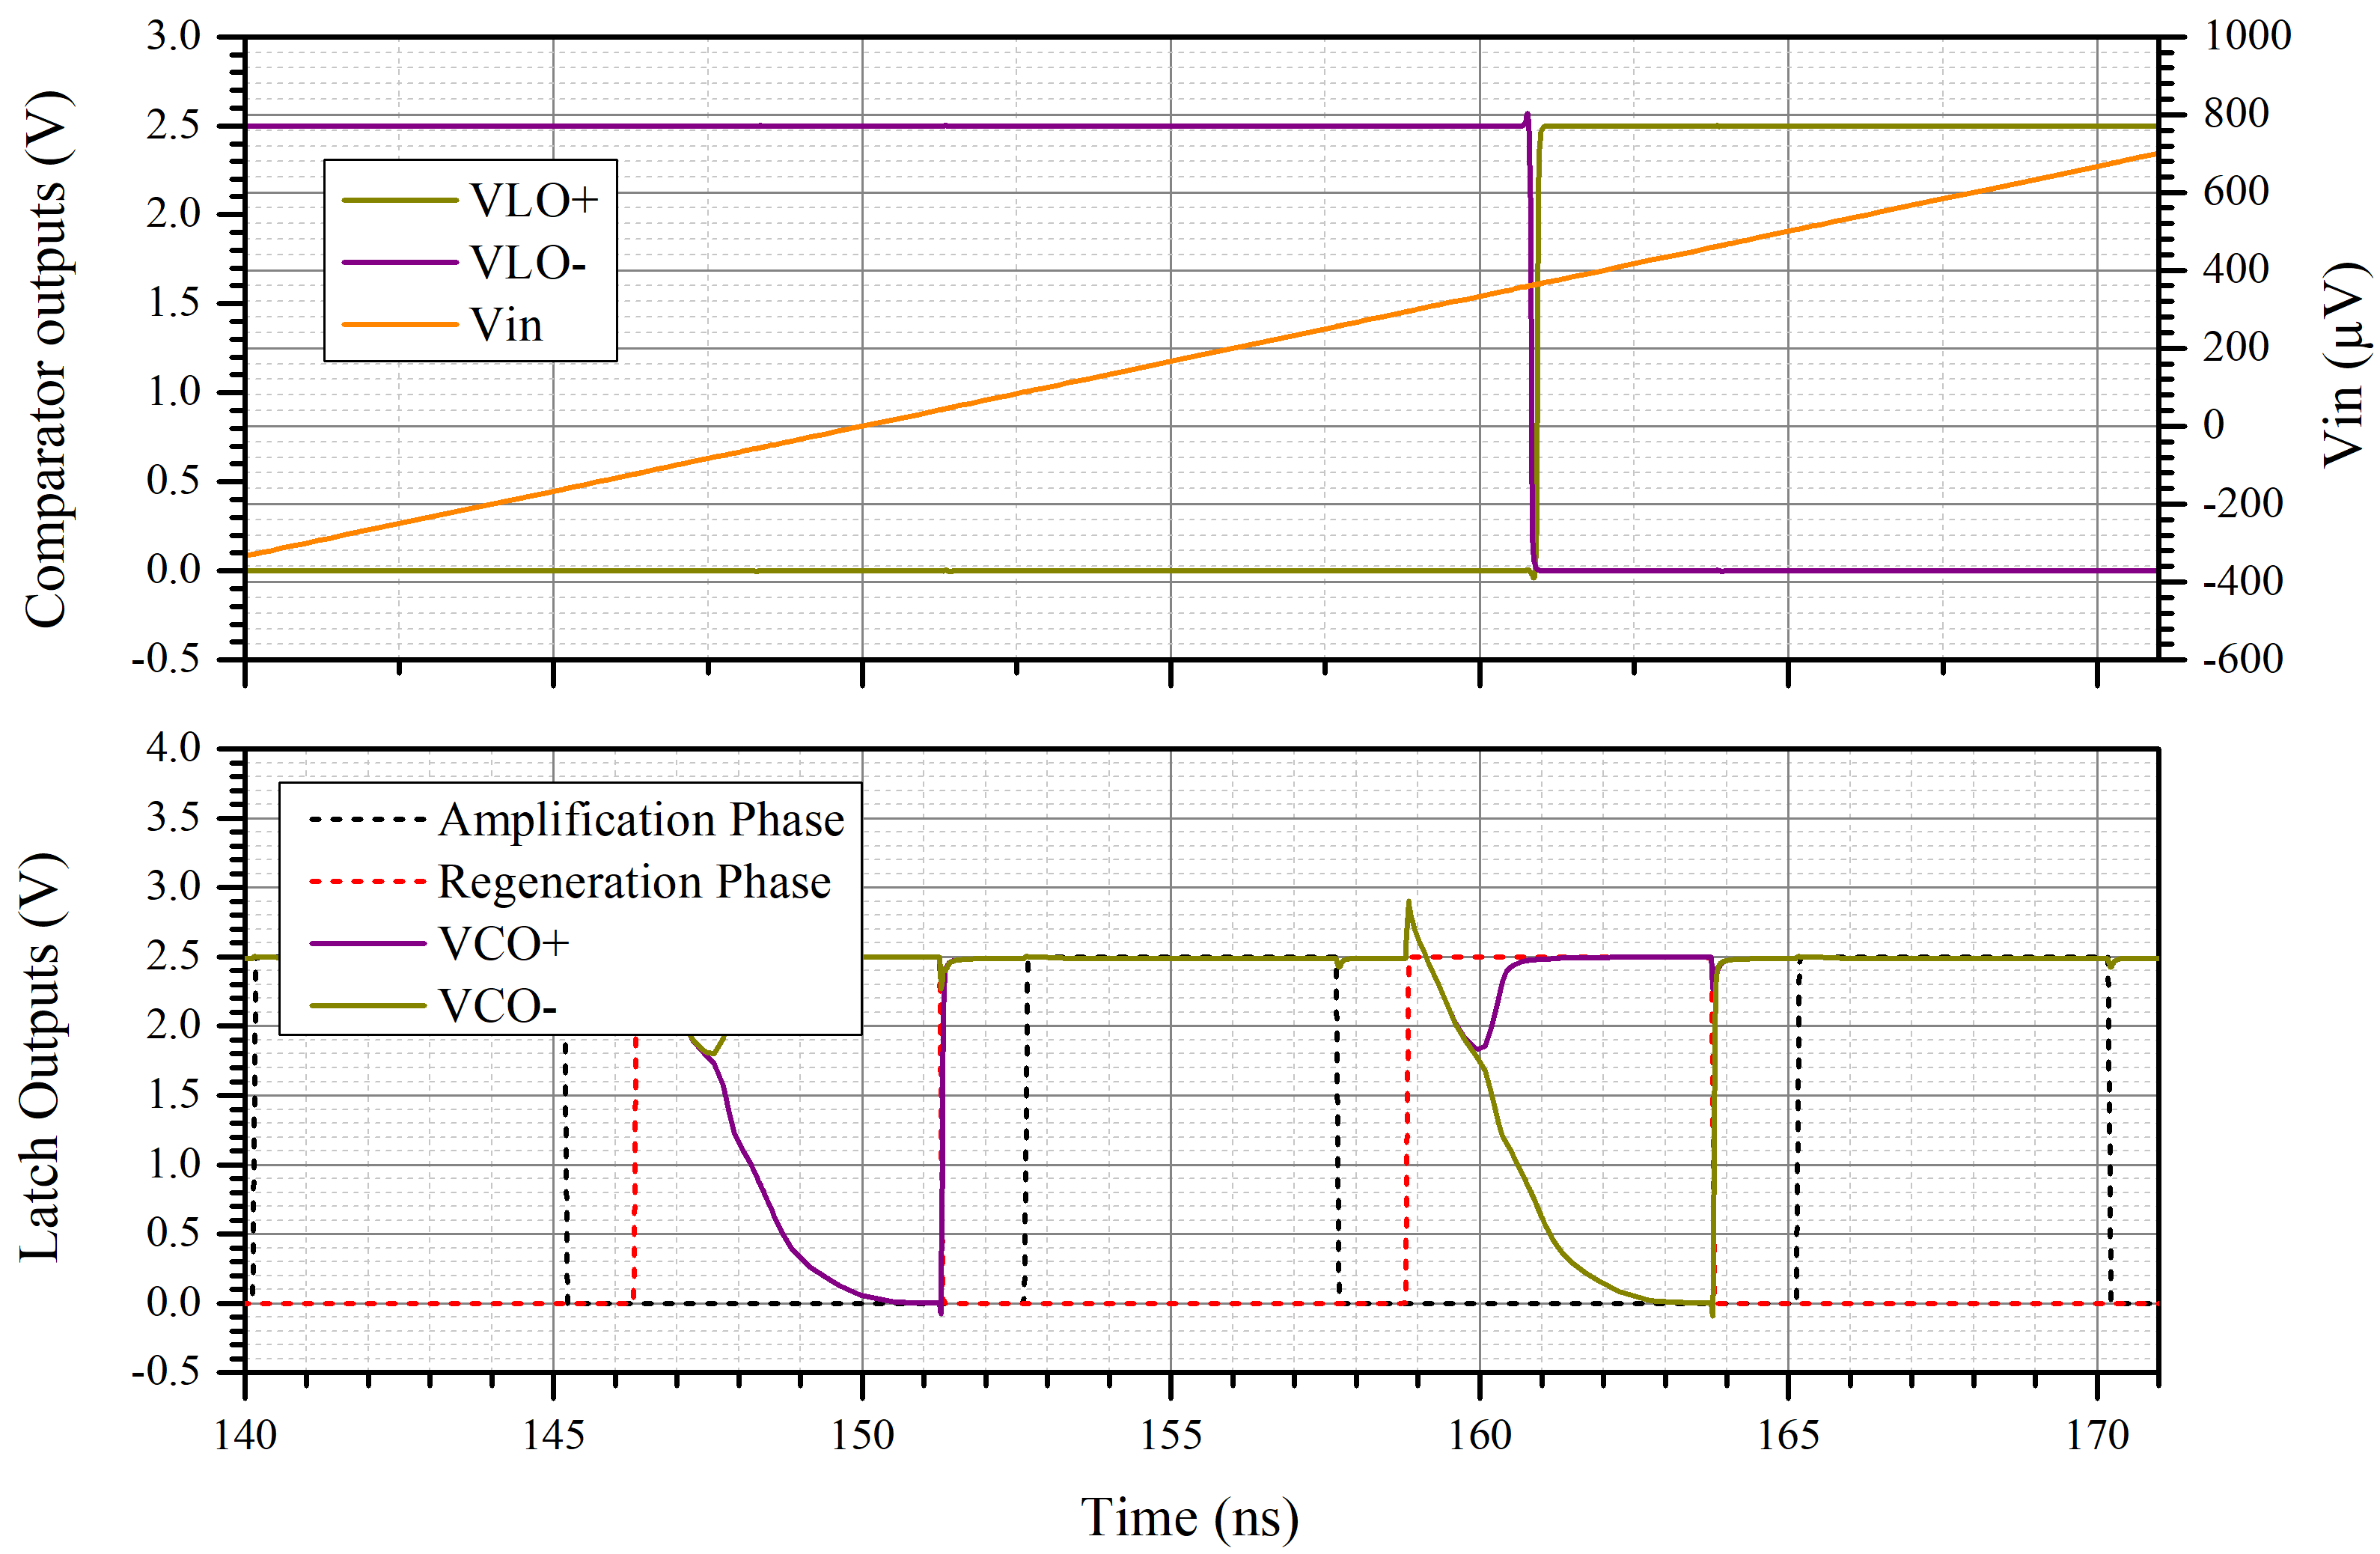
\includegraphics[width=\columnwidth]{Chap05/Figures/comparator_signals.png}
\caption{Signals at the different nodes of the Comparator}
\label{fig:comp_sigs}
\end{figure}
The simulation results of the comparator in Fig. \ref{LATCH} are shown in the Fig. \ref{fig:comp_sigs}. In the simulation set-up the negative terminal of the comparator ($V_{in}^-$) is kept constant at the common-mode voltage ($V_{CM}=1.25~V$) while the positive terminal ($V_{in}^+$) is linearly varied from ($V_{CM}-10~mV$) to ($V_{CM}+10~mV$), while the comparator is clocked at the frequency of 80~MHz. The characteristic in orange in the top plot shows the differential input voltage ($V_{in}^+-V_{in}^-$) in the time frame from $140~ns$ to $171~ns$ which covers two amplification phases and two regeneration phases. In the first amplification phase, from time $140~ns$ to $145~ns$, the differential input voltage is around $-300~\mu V$. Therefore in the regeneration from $146~ns$ to $151~ns$, higher potential on the negative input causes to draw the more current through transistor $M_1$ than that through $M_0$. The rate at which the positive output node ($V_{CO}^+$) is discharging is higher than that the negative node ($V_{CO}-$) discharge rate. In turn, the node $V_{CO}+$ reaches the potential of $V_{DD}-V_{thp}$ first, which is connected to the gate of the transistor $M_4$ turning it $on$ thereby connecting the $V_{DD}$ to the negative output $V_{CO}^-$. This output is connected to the gate of NMOS transistor $M_3$ causing it to turn $on$ and the gate of PMOS transistor $M_5$ turning it $off$ which discharges the node to ground very fast. These outputs from comparator are then provided to the SR latch which stores the decision with outputs $V_{LO}^+$ and $V_{LO}^+$ as shown in the top plot of Fig. \ref{fig:comp_sigs}.

In the next amplification phase, the differential input is positive and is around $200~\mu V$. Therefore exactly counter-operation in the comparator will take place in regeneration phase pulling the $V_{CO}^-$ to ground and pushing $V_{CO}^+$ node to $V_{DD}$ as shown in the bottom plot of the Fig. \ref{fig:comp_sigs}.
\begin{figure}[h]
\centering
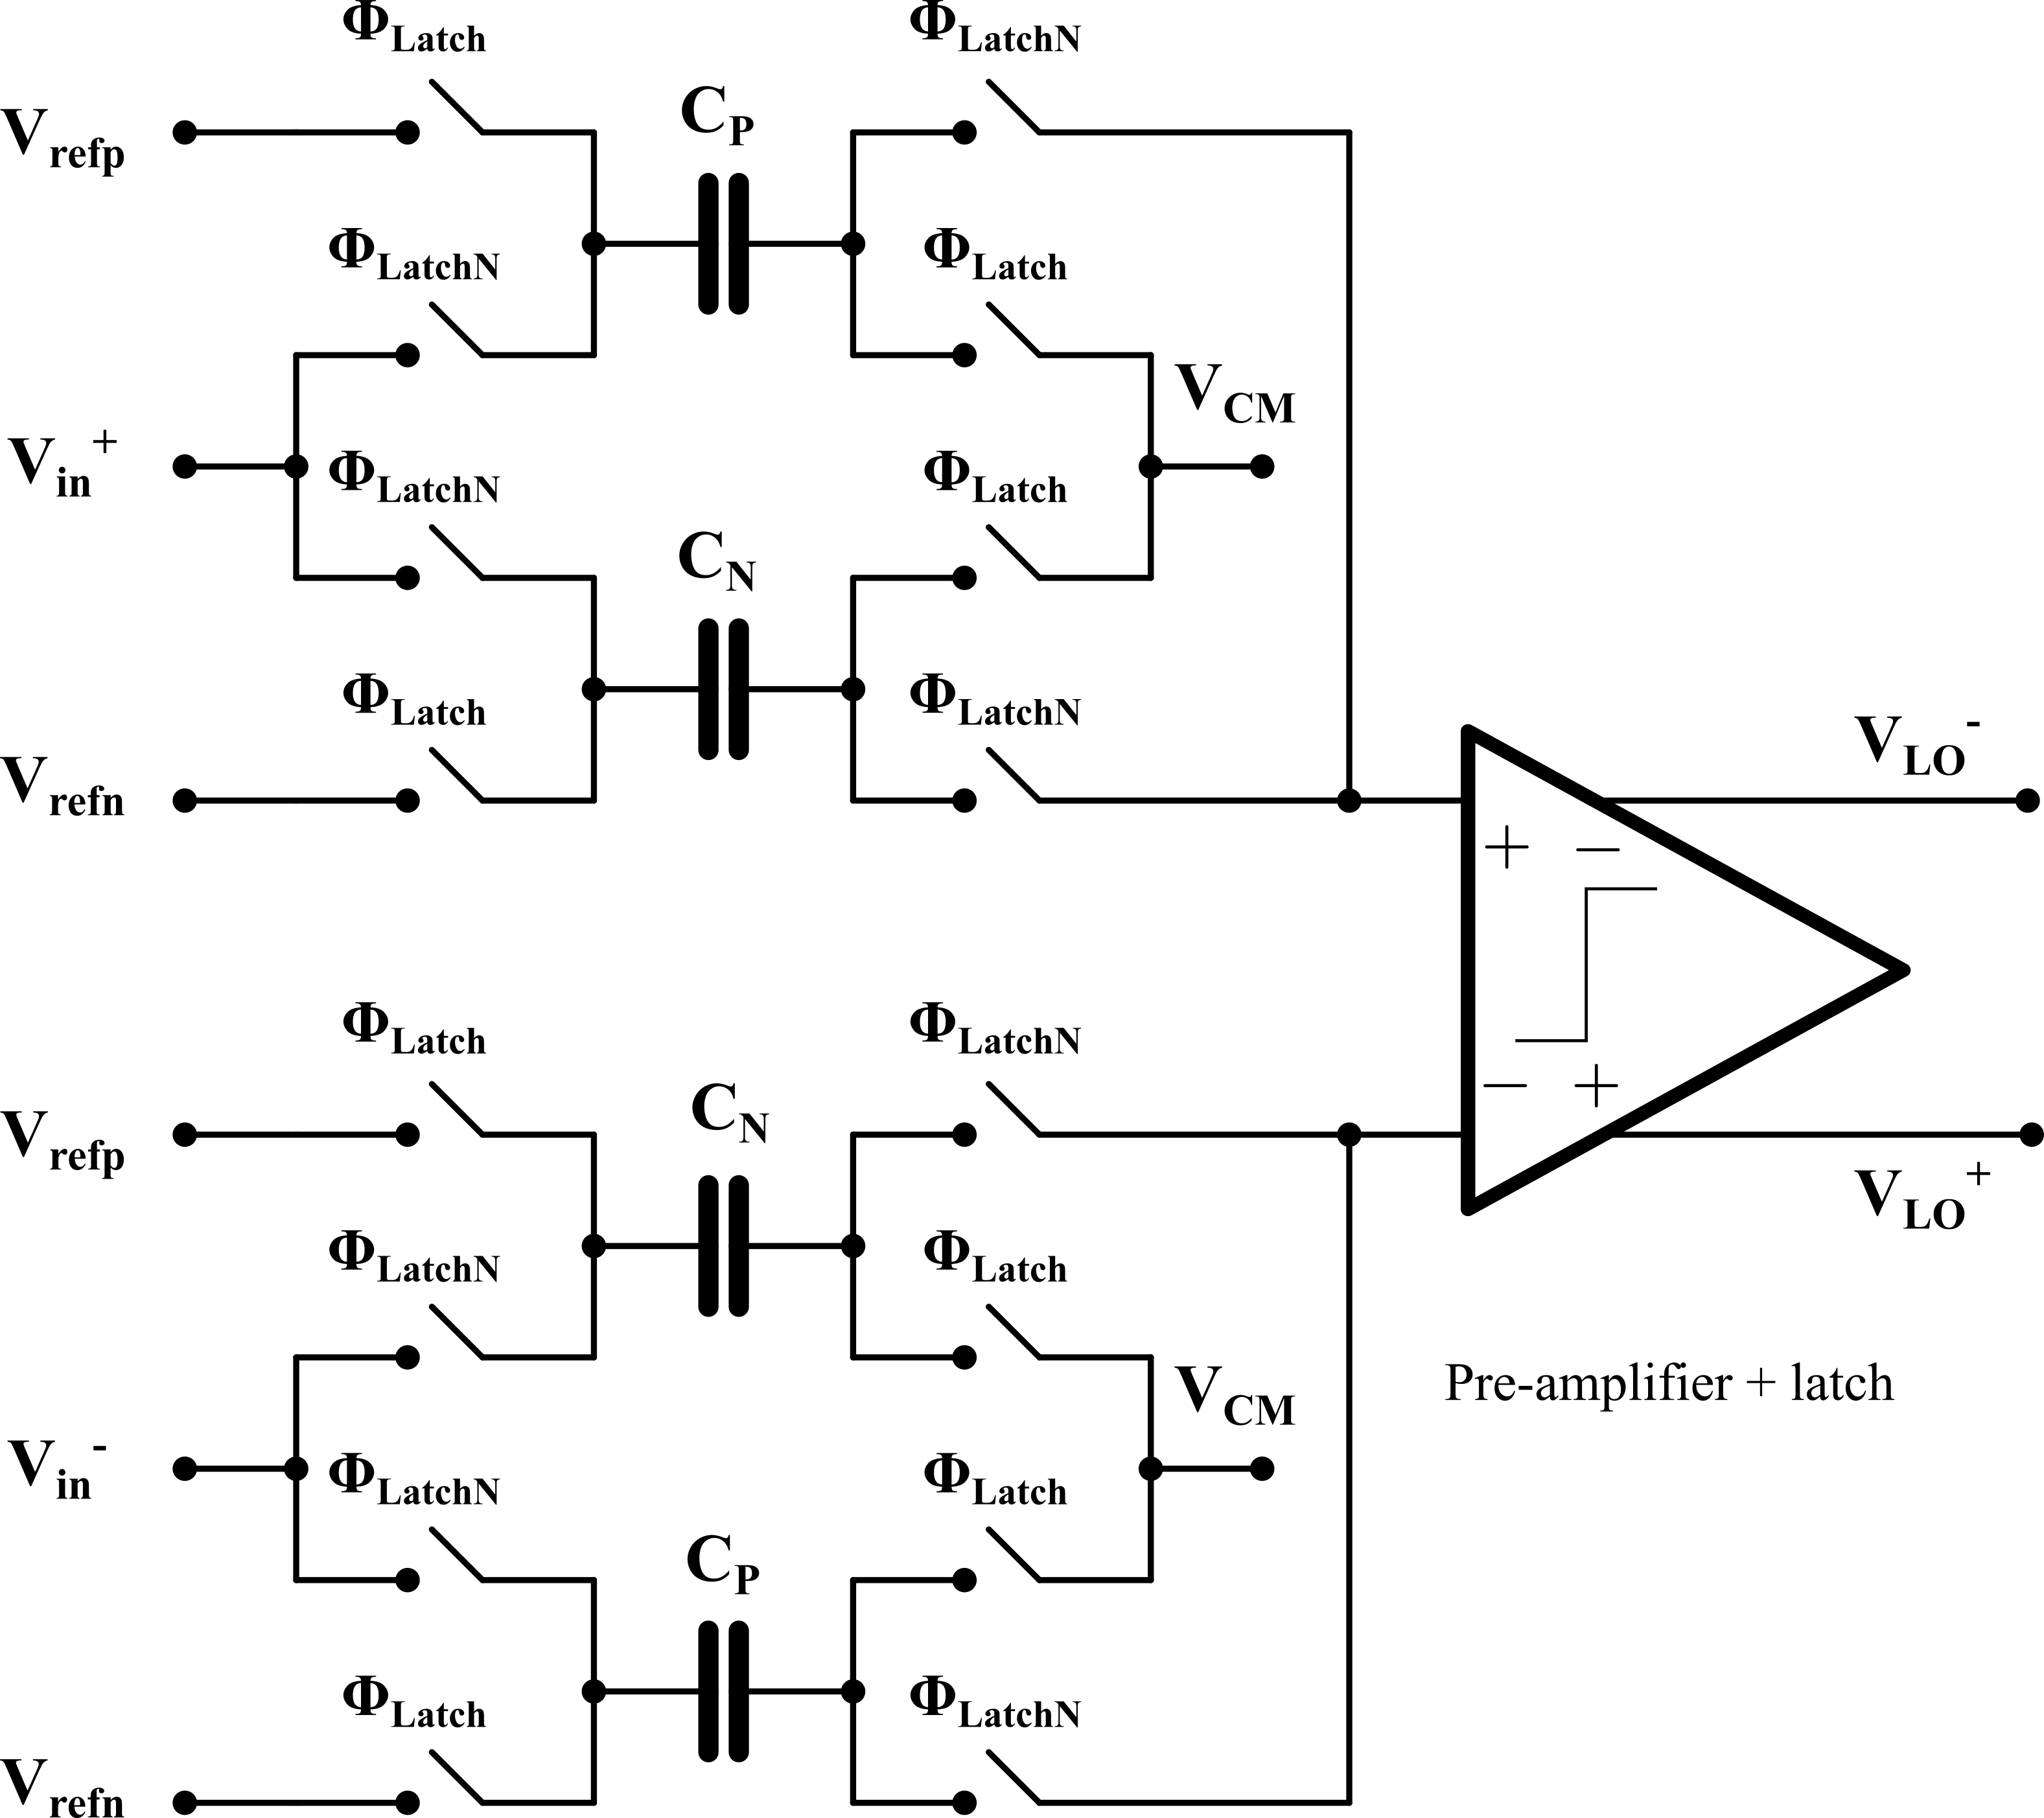
\includegraphics[width=0.75\columnwidth]{Chap05/Figures/comp_thr.png}
\caption{A complete structure of Comparator}
\label{COMP_THR}
\end{figure}

A complete structure of the comparator is shown in Fig. \ref{COMP_THR} which consists of a switched-capacitor threshold generator and the next block is pre-amplifier and the back-to-back connected NOT for amplification and regeneration. This is the one slice of the whole quantizer. In case of 3-bit quantizer, there will be such a 7 slices with different values of $C_P$ and $C_N$ generating 7 different thresholds as shown in Tab. \ref{tab:vthr_mod}.
\section{DAC Architecture}
\begin{figure}[h]
\centering
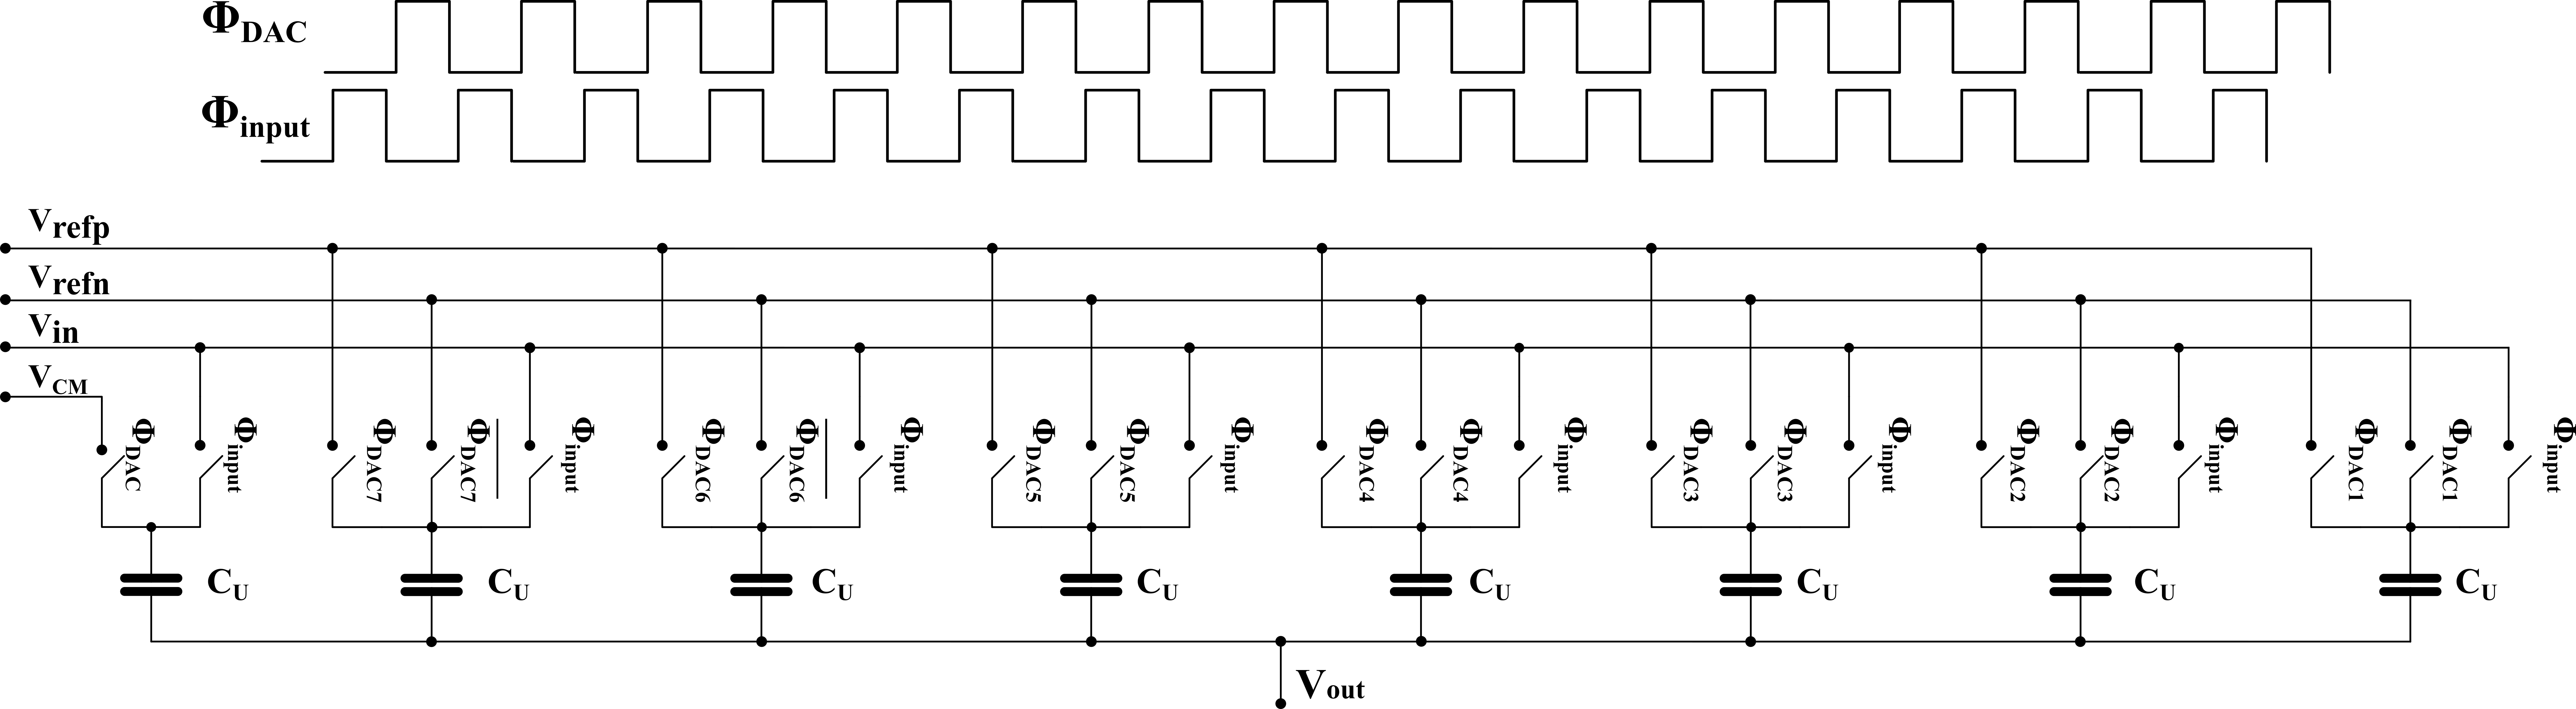
\includegraphics[width=\columnwidth]{Chap05/Figures/dac.png}
\caption{A 3-bit Thermometric Capacitive DAC at the input of First integrator}
\label{DAC}
\end{figure}
Since, the quantizer implemented in the IADC is of the resolution of 3-bit, the architecture of the DAC employed needs to be of the same resolution. Therefore the capacitive DAC with thermometric inputs is realized as shown in the Fig. \ref{DAC}. In the phase $\Phi_{input}$, the input signal is sampled on the array of unit capacitors comprising the sampling capacitor while in the phase $\Phi_{DACn}$, the feedback signal from the quantizer is sampled and thus a difference between input signal and the digital equivalent of the input signal i.e. residue is integrated.
Here, $\Phi_{DACn} = \Phi_{DAC}*b_n$ and $\overline{\Phi_{DACn}} = \Phi_{DAC}*\overline{b_n}$ where $b_n$ and $\overline{b_n}$ are the $n^{th}$ thermometric output and it's complement from the quantizer and the $\Phi_{DAC}$ is the phase when feedback DAC signal should be applied. 


\section{Inter-Stage Gain Block}

\begin{figure}[h!]
% \centering
\hspace{1in}
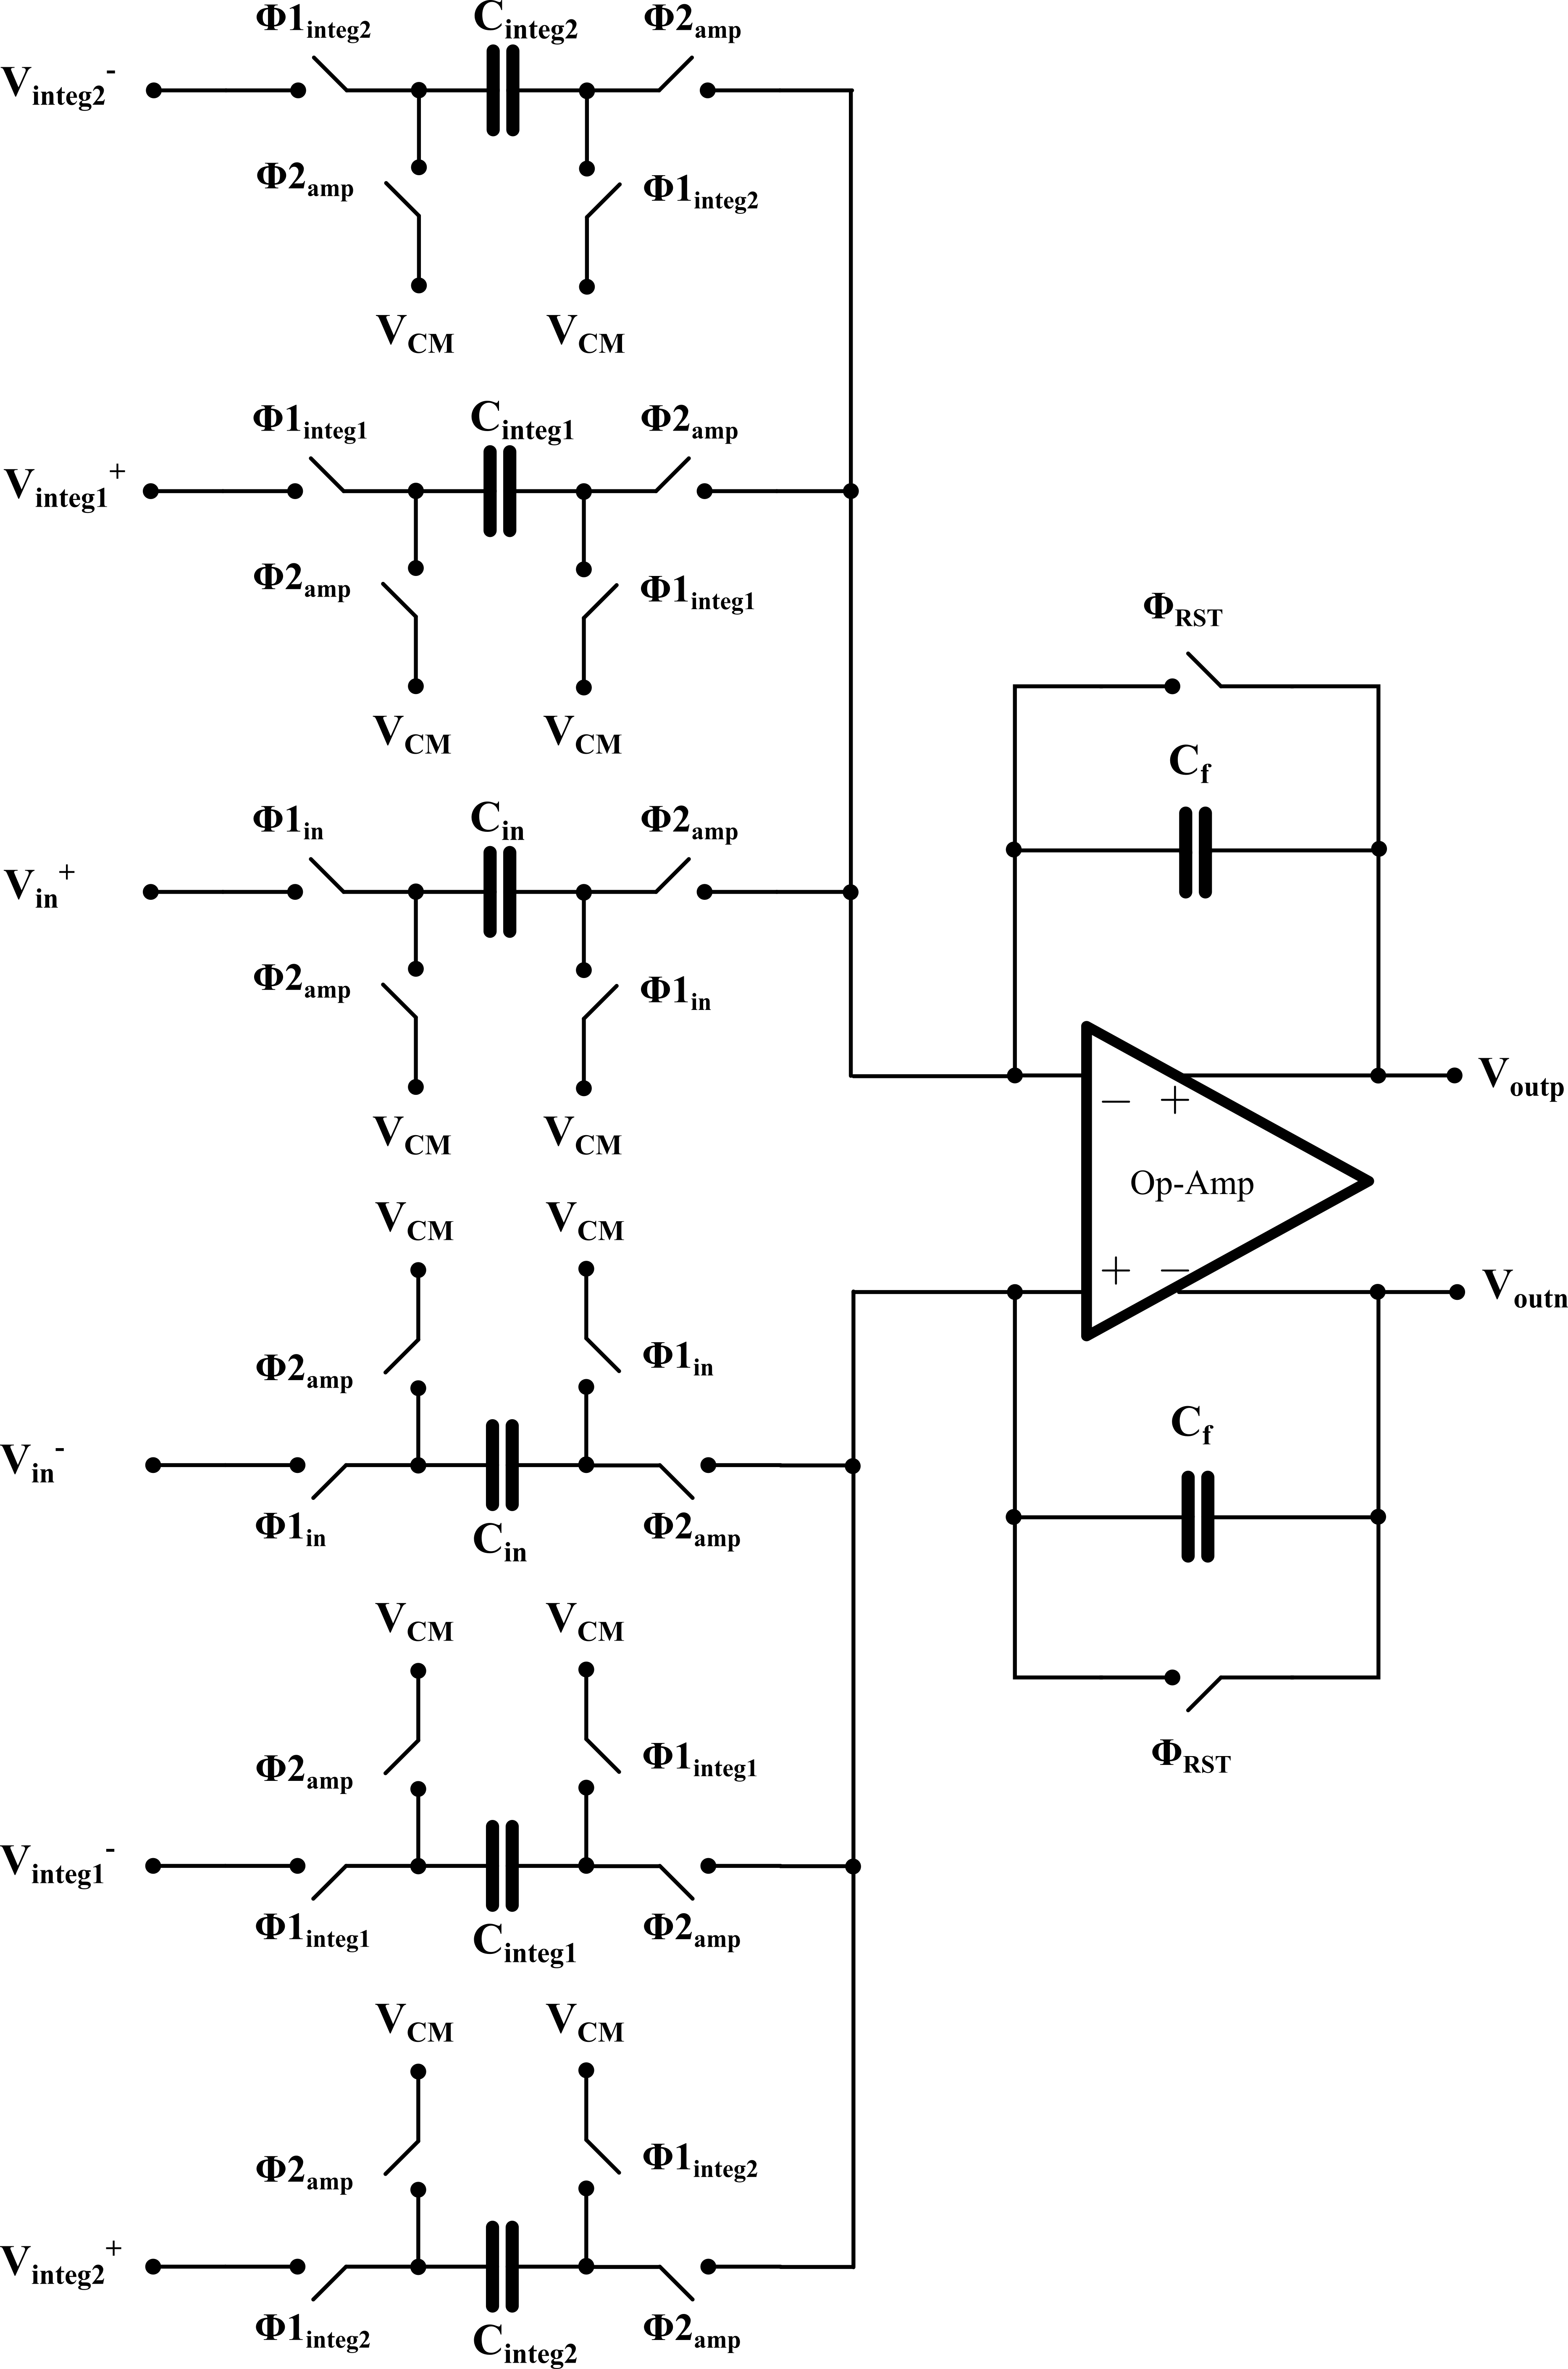
\includegraphics[width=0.7\columnwidth]{Chap05/Figures/ISG.png}
\caption{Inter-Stage Gain Block Diagram}
\label{fig:ISG}
\end{figure}

The circuit diagram of the Inter-stage Gain block is shown in Fig.~\ref{fig:ISG}. Since the architecture employed is the modified architecture of the Incremental ADC, the output of the second integrator contains not only the residue but the components proportional to the input signal as well as the output of the first integrator.
%
\begin{equation*}
        y[M]=a_1u[M]+a_2w[M]+a_1a_2\frac{M(M-1)}{2}u-a_1a_2V_{ref}\left(v[M-2]+.....+(M-1)v[0]\right)
\end{equation*}
%
Where the integrator coefficients $a_1=1$ and $a_2=1$ and the feed-forward coefficients $b_1=1$ and $b_2=2$. 

Therefore the ISG block has to first extract the residue by subtracting the input signal and the output of the first integrator from the second integrator's output with proper coefficients and then amplify the residue so as to cover the full-scale of the residual ADC (RADC), i.e.
%
\begin{equation}
    e[M]=y[M]-b_1u[M]-b_2w[M]
\end{equation}
%
%
\begin{equation}
    ISG\ output = G e[M] = G y[M]-G b_1u[M]-G b_2w[M]
\end{equation}
%
Then, the coefficients $b_1=1$ and $b_2=2$ are set by the IADC part while the ISG gain $G$ must be set to $2^{N_{SD}-1}$, i.e. 4, so that the amplified residue covers full-scale of RADC. Then the final coefficients of the input signal $u[M]$, output of first integrator $w[M]$ and the output of second integrator $y[M]$ for the extraction and amplification of residue are constructed by the ratio of the sampling capacitor and the feedback capacitors i.e.
%
\begin{equation}\label{eq:isg_caps}
    \begin{split}
        Coeff.\ of\ y[M]&=\frac{C_{integ2}}{C_F}=4\\
        b_1&=\frac{C_{input}}{C_F}=4\\
        b_2&=\frac{C_{integ1}}{C_F}=8
    \end{split}
\end{equation}
%
However, it should be noted that, the second integrator's output is already reduced by factor of 4 in order to satisfy the swing of the op-amp. Therefore the signals $y[M]$, $u[M]$ and $w[M]$ are smaller by factor of 4. Thus, if the residue has to be amplify to the RADC full-scale (1.2V), the additional amplification factor must be incorporated in inter-stage gain $G$, i.e. overall gain factor will be 16 and the swing will be then 1.2V. 

Nevertheless, it has been seen that achieving such a high voltage swing for given low frequency gain of 50~dB and GBW of 200~MHz is quite difficult. Hence, the ISG gain is set to 4 instead, which brings the residue swing down. Then the capacitance ratios are as shown in the Eq.(\ref{eq:isg_caps})

Note that the residue swing is now $1/4^{th}$ of the reference voltage. It means the overall ERADC signal-to-quantization noise ratio will go down by 12~dB.
%
\begin{figure}[h!]
    \centering
    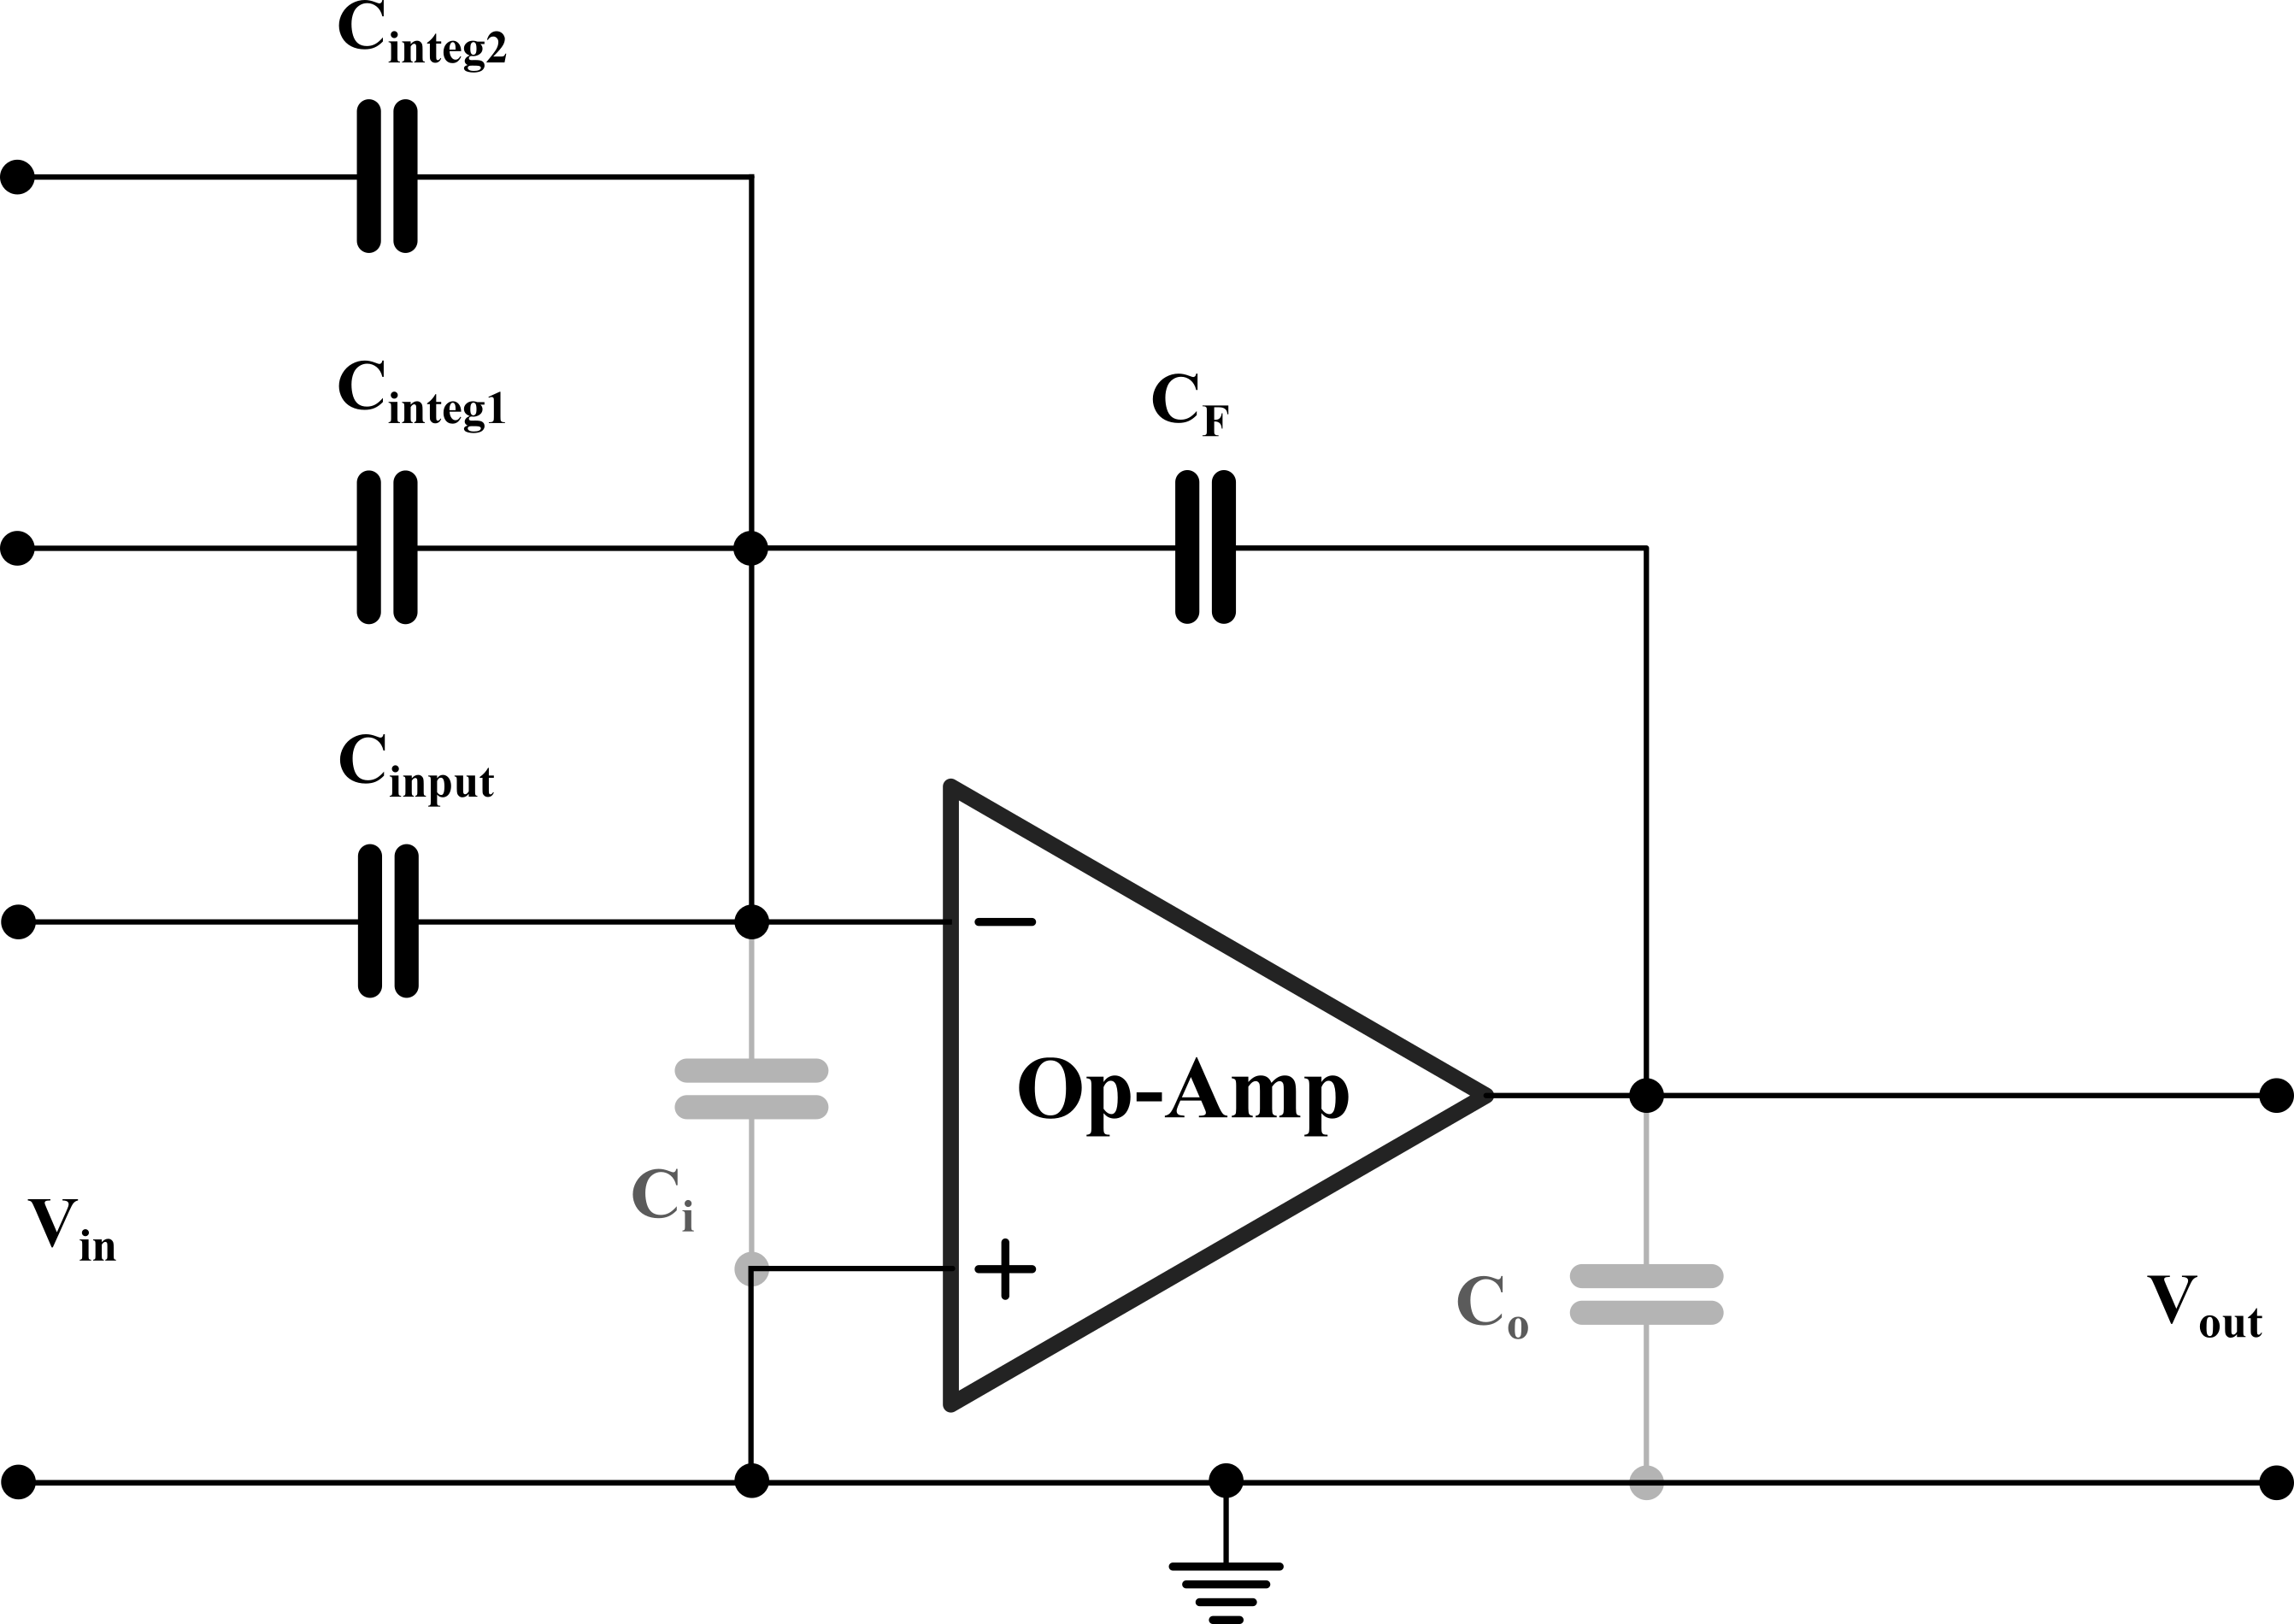
\includegraphics[width=0.6\columnwidth]{Chap05/Figures/ISG_opamp.png}
    \caption{Single ended representation of the Inter-stage Gain Block in the amplification phase}
    \label{fig:ISG_ampl}
\end{figure}
%

After considering the parasitic capacitance at virtual ground and the output node, the configuration of ISG in the integrating phase looks like as shown in Fig. \ref{fig:ISG_ampl}. Then the total load capacitance and the beta factor can be calculated as,
%
\begin{equation}
    C_{L_{ISG}}=\frac{C_{F}(C_{input}+C_{integ1}+C_{integ2}+C_i)}{C_{F}+C_{input}+C_{integ1}+C_{integ2}+C_i}+C_o
\end{equation}
%
%
\begin{equation}
    \beta_{ISG} = \frac{C_{F}}{C_{F}+C_{input}+C_{integ1}+C_{integ2}+C_i}
\end{equation}
%
The values of the capacitances are $C_{input}=C_{integ2}=400 fF$, $C_{integ1}=800 fF$ while $C_{F}=100 fF$. The parasitics considered prior to the design $C_i=100f$
and $C_o=100f$, which results in the total load capacitance of around $200 fF$ and the feedback factor $\beta = \frac{1}{18}$. However, the op-amp requirements are quite similar to that in the first integrator. Therefore, the similar architecture is employed for the amplifier also in the ISG for the specifications of low-frequency loop gain = 60~dB, and the GBW = 200~MHz for given load and the feedback factor.


\section{Supporting Blocks}
The two integrators, multi-bit quantizer, feedback DAC and the inter-stage gain block are the core blocks of the ERADC architecture where the functionality of the structure can be verified. However, few more blocks are needed to incorporate along with core blocks such as biasing block which is used to bias the op-amps in the integrators and the inter-stage gain block as well as the comparators in the quantizer, the timing block to generate various phases such as $\Phi_1$, $\Phi_2$ etc and some spacial signals such as End-of-Conversion ($\Phi_{EOC}$), reset integrators ($\Phi_{RST}$), the Dynamic Element Matching (DEM) to improve the linearity of the feedback DAC etc.

\subsection{Biasing}
There are op-amps in the two integrators and the ISG block and the comparators in the quantizer which need the biasing current of $10~\mu A$. Therefore a biasing circuit is developed as shown in Fig. \ref{fig:bias} which does the job.
%
\begin{figure}[h!]
\centering
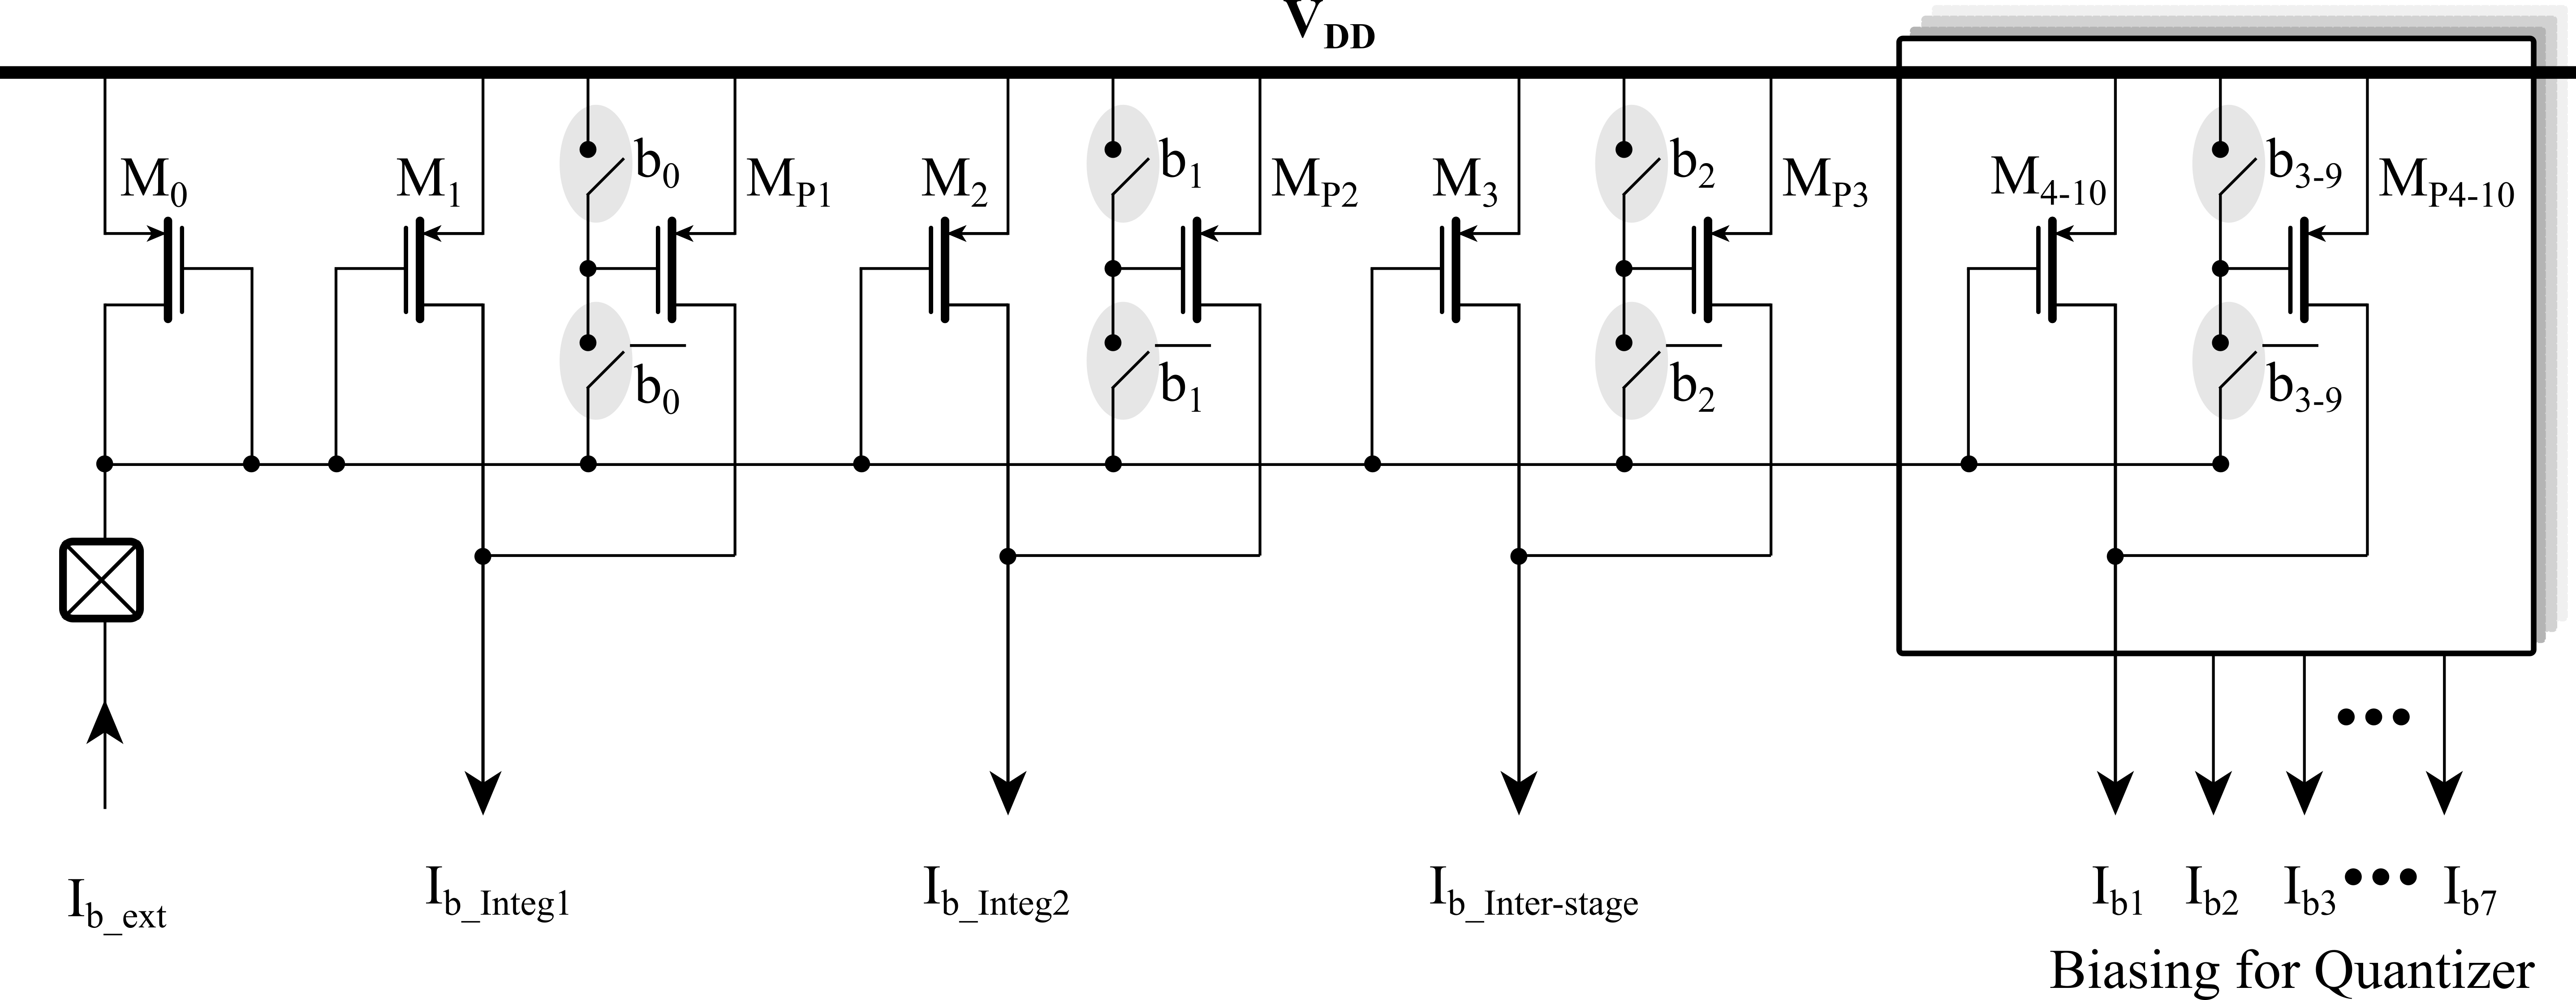
\includegraphics[width=\columnwidth]{Chap05/Figures/biasing_block.png}
\caption{Programmable Biasing Block Diagram}
\label{fig:bias}
\end{figure}
%
%
\begin{figure}[h]
\centering
\subfigure[]{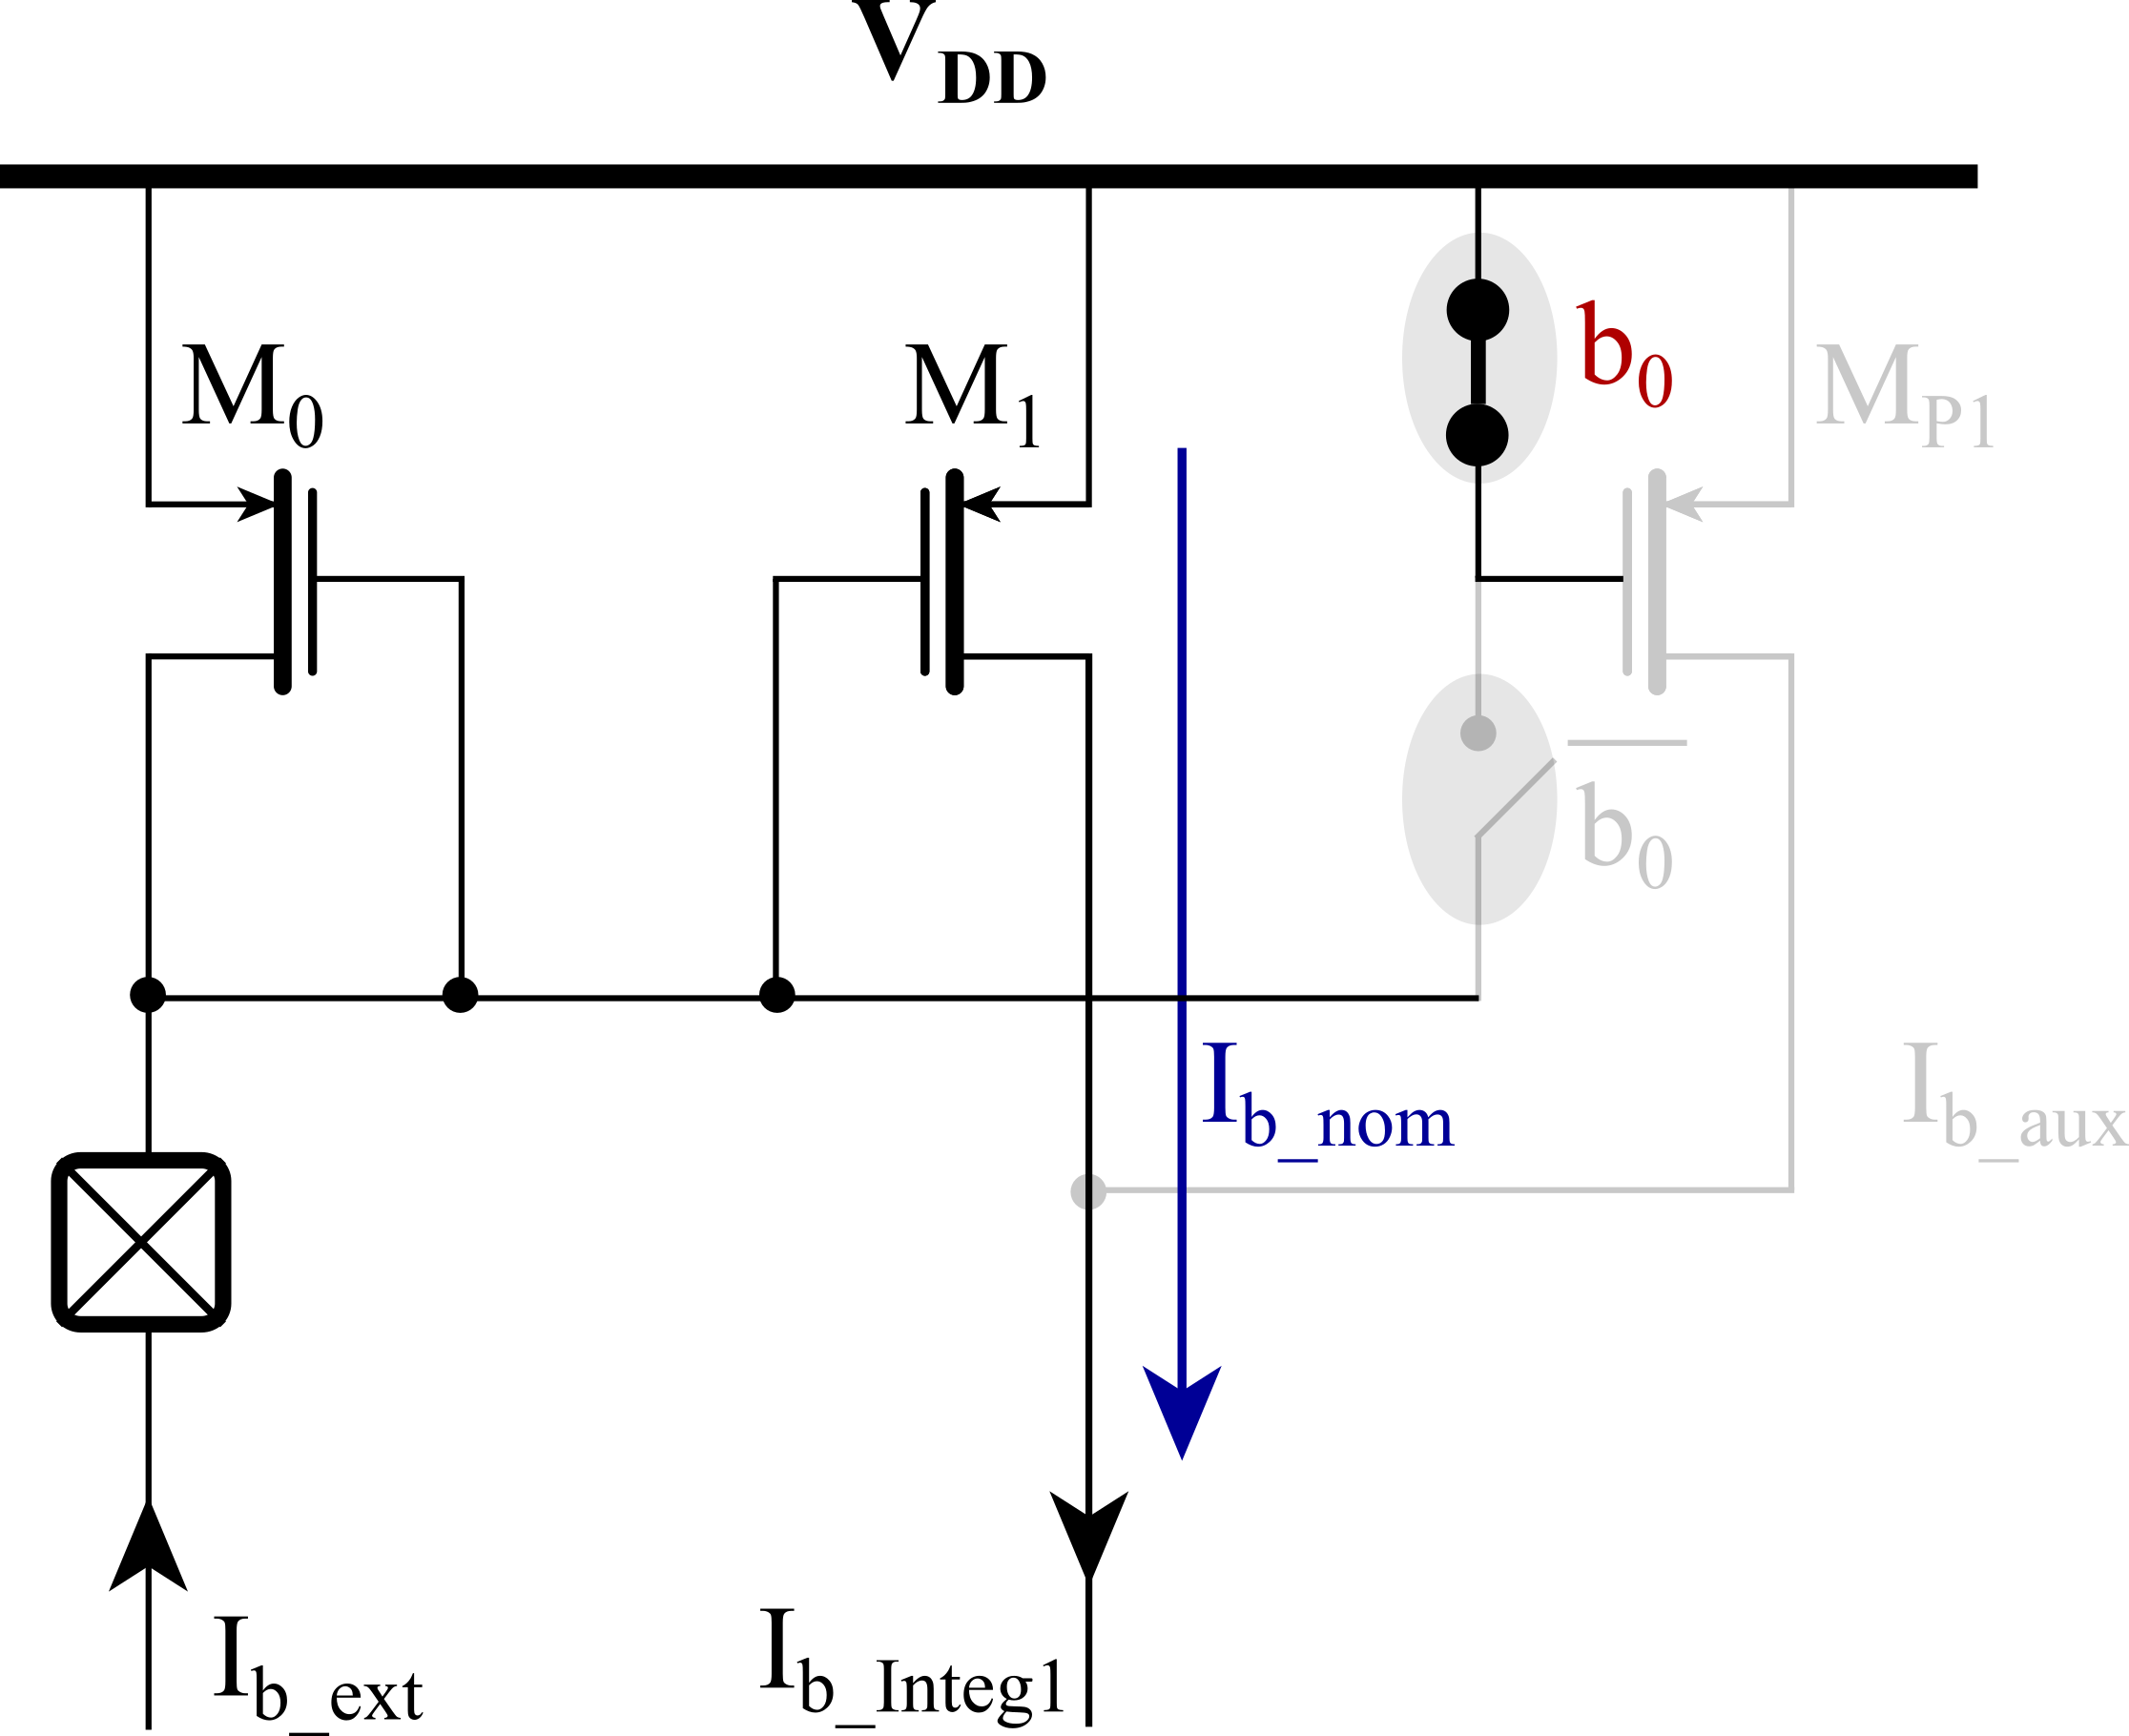
\includegraphics[scale=.33]{Chap05/Figures/biasing_block11.png}}
\qquad
\subfigure[]{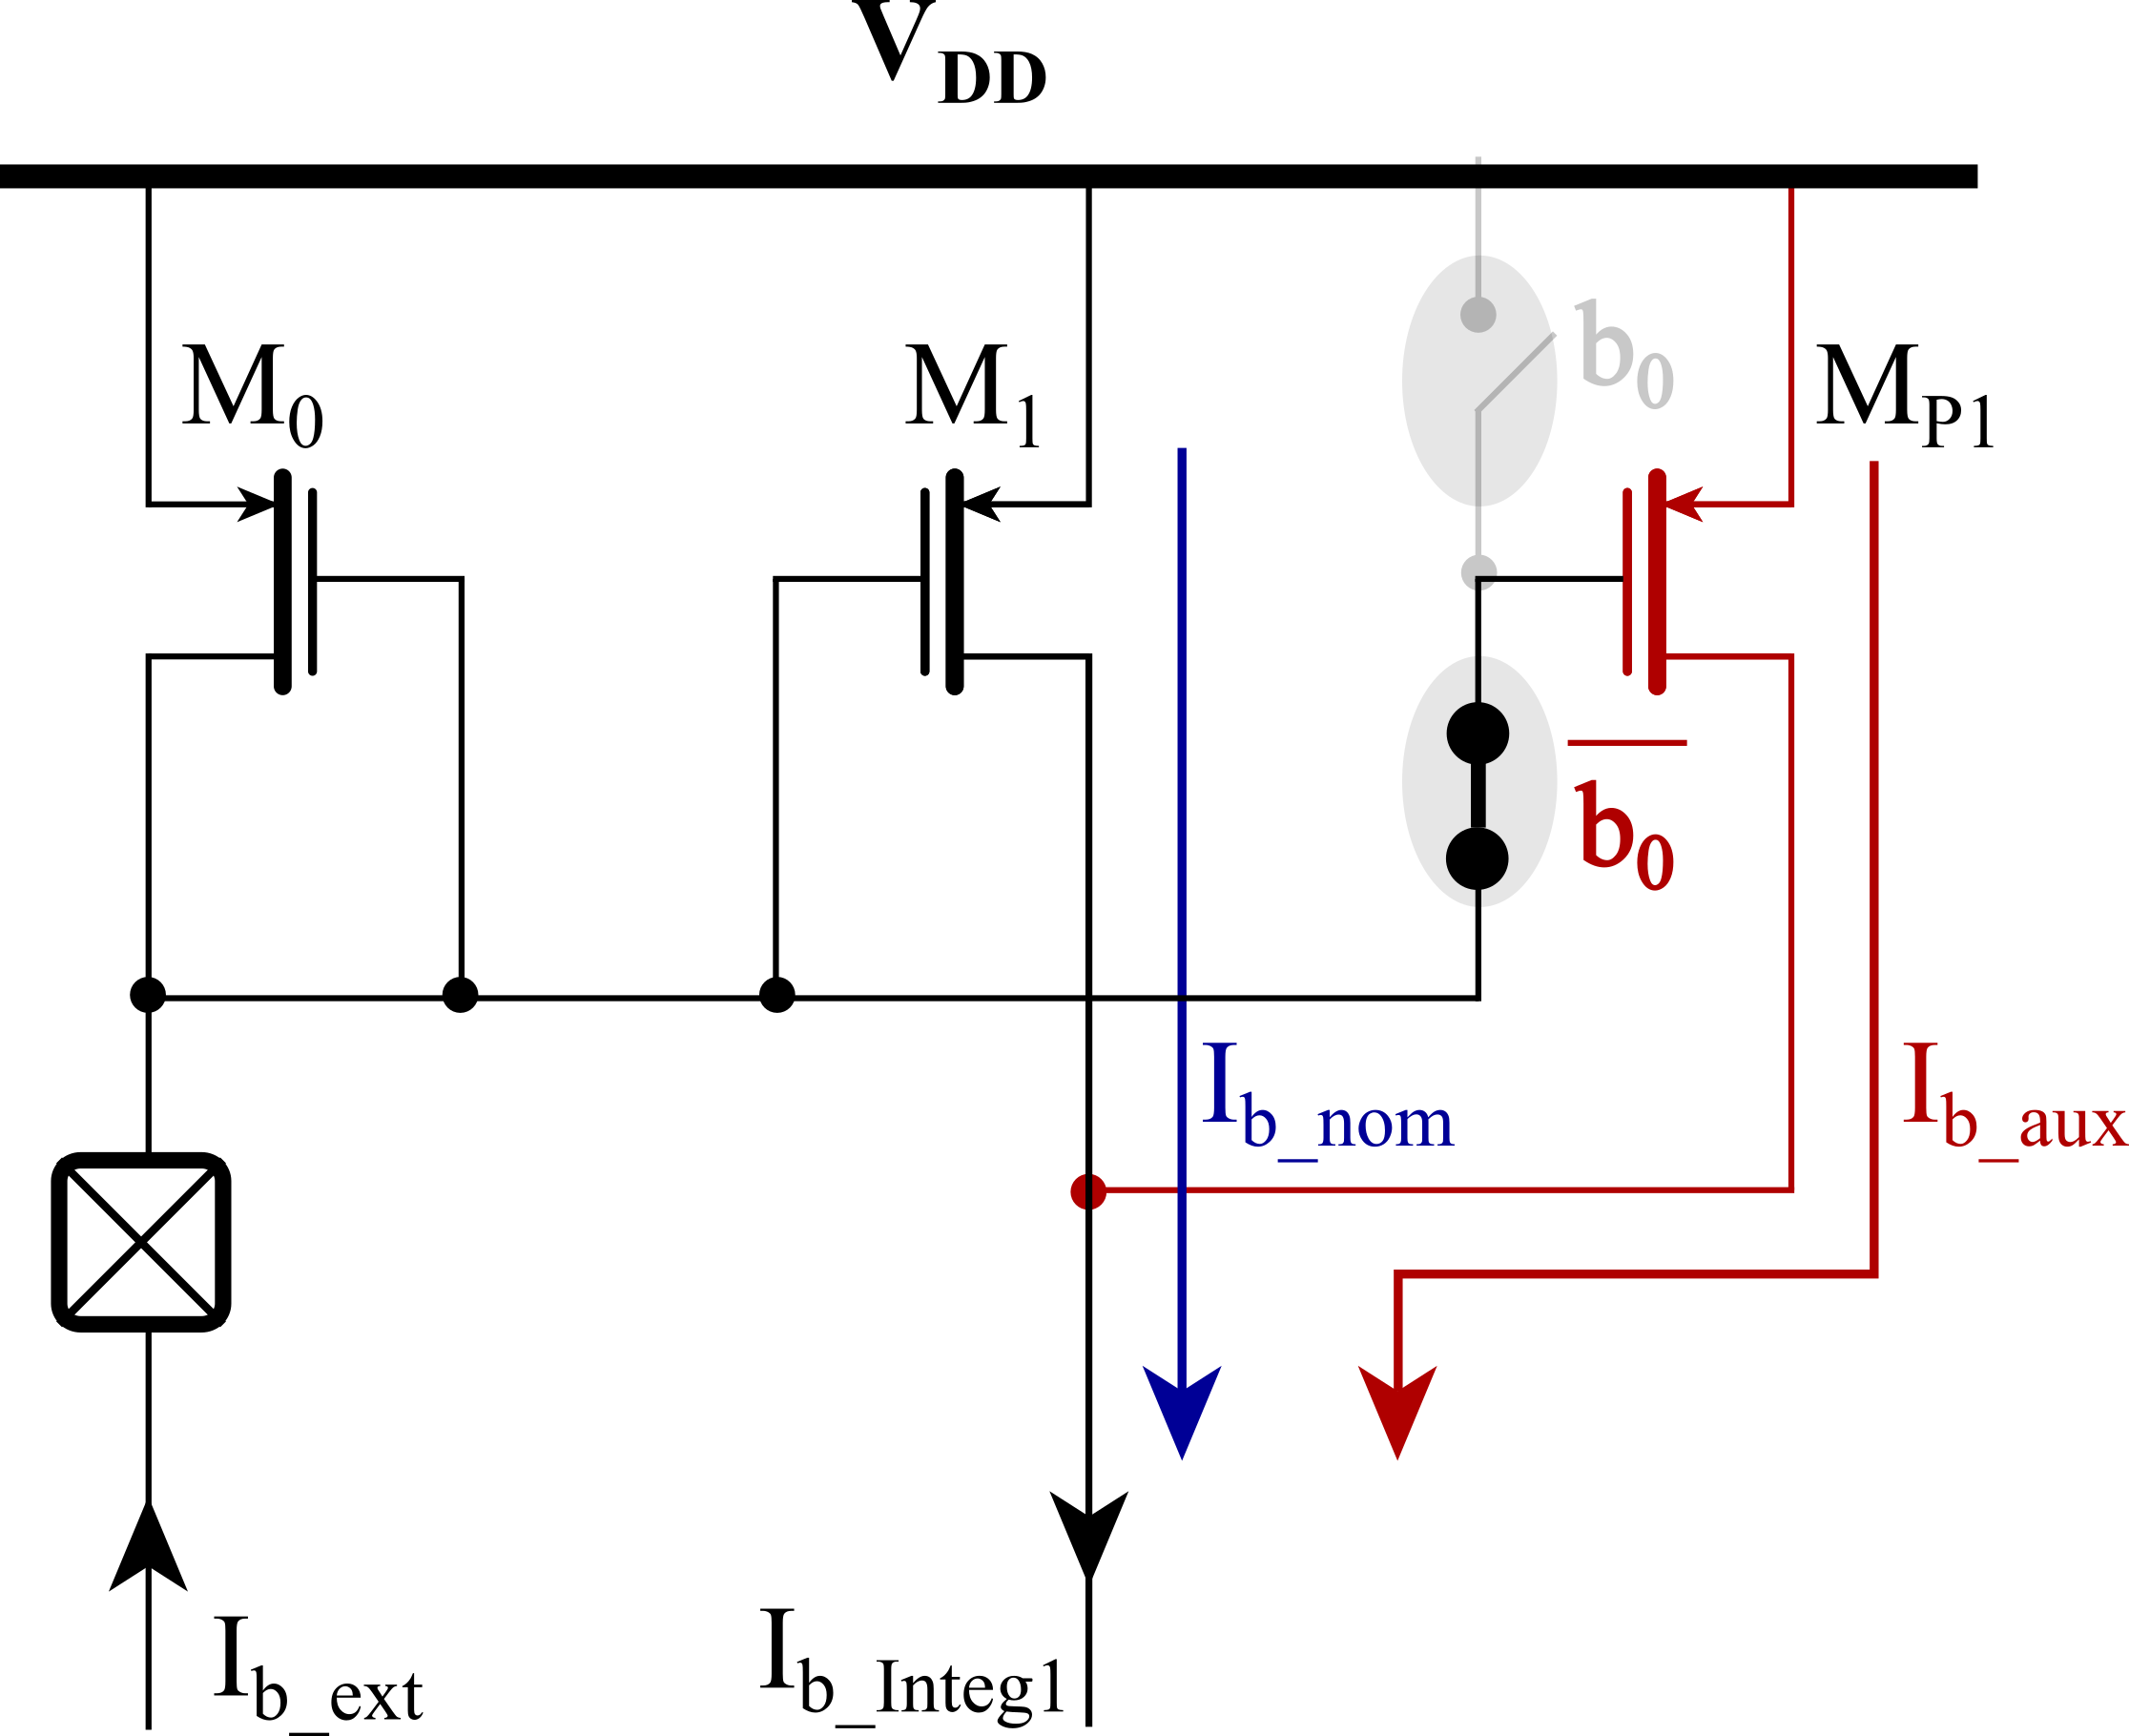
\includegraphics[scale=.33]{Chap05/Figures/biasing_block22.png}}
\caption{(a) Typical bias current: programming bit disables additional current (b) Higher bias Current: programming bit enables additional current}
\label{fig:bias_1}
\end{figure}
%
It needs an external biasing current of $10~\mu A$ draining from $V_{DD}$ through the diode connected transistor $M_0$ which generates the corresponding voltage $V_{SG}$ across it's source-to-gate. This voltage is then utilized to create the multiple copies of the biasing current. The dimensions of the transistors are similar to the $M_0$ i.e. $\left(\frac{W}{L}\right)_0=\left(\frac{W}{L}\right)_{1-10}=3\left(\frac{W}{L}\right)_{P1-P10}$ Transistor $M_1$, $M_2$, $M_3$ is used to bias the op-amps in the first integrator, second integrator and inter-stage gain block respectively while those from $M_4$ to $M_{10}$ biases the seven comparators in the quantizer. Furthermore, all the biasing current sources are made programmable through additional current source transistors $M_{P1}$ to $M_{P10}$ by programming bit $b_0$ to $b_9$ to have a flexibility to draw more current if needed by any particular block. When the programming bit is low, the gate of the transistors are connected to the $V_{DD}$ bringing it's $V_{SG}$ to $0~V$ turning it \textit{OFF} hence drawing zero current through the auxiliary source. Thus the nominal current is delivered.

The dimensions of the auxiliary current sources ($M_{P1}-M_{P10}$) are such a that they can add $30\%$ more current to the main current sources. 
%
\begin{figure}[h!]
\centering
\includegraphics[width=\columnwidth]{Chap05/Figures/dwa_circuit.png}
\caption{Data Weighted Averaging (DWA) implementation approach}
\label{fig:dwa}
\end{figure}
%
\subsection{Dynamic Element Matching (DEM)}
In case of multi-bit digital-to-analog converter (DAC), due to the process variations, there is a mismatch between the unit elements. This mismatch causes the DAC levels to deviate from the ideal ones, which in turn makes the input-output characteristic of the DAC non-linear. Therefore, if the sinusoidal signal is passed through this non-linear function, it gives rise to the harmonics, significantly reducing the SNR, usually called signal-to-noise and distortion ratio (SNDR).
%
\begin{figure}[h!]
\centering
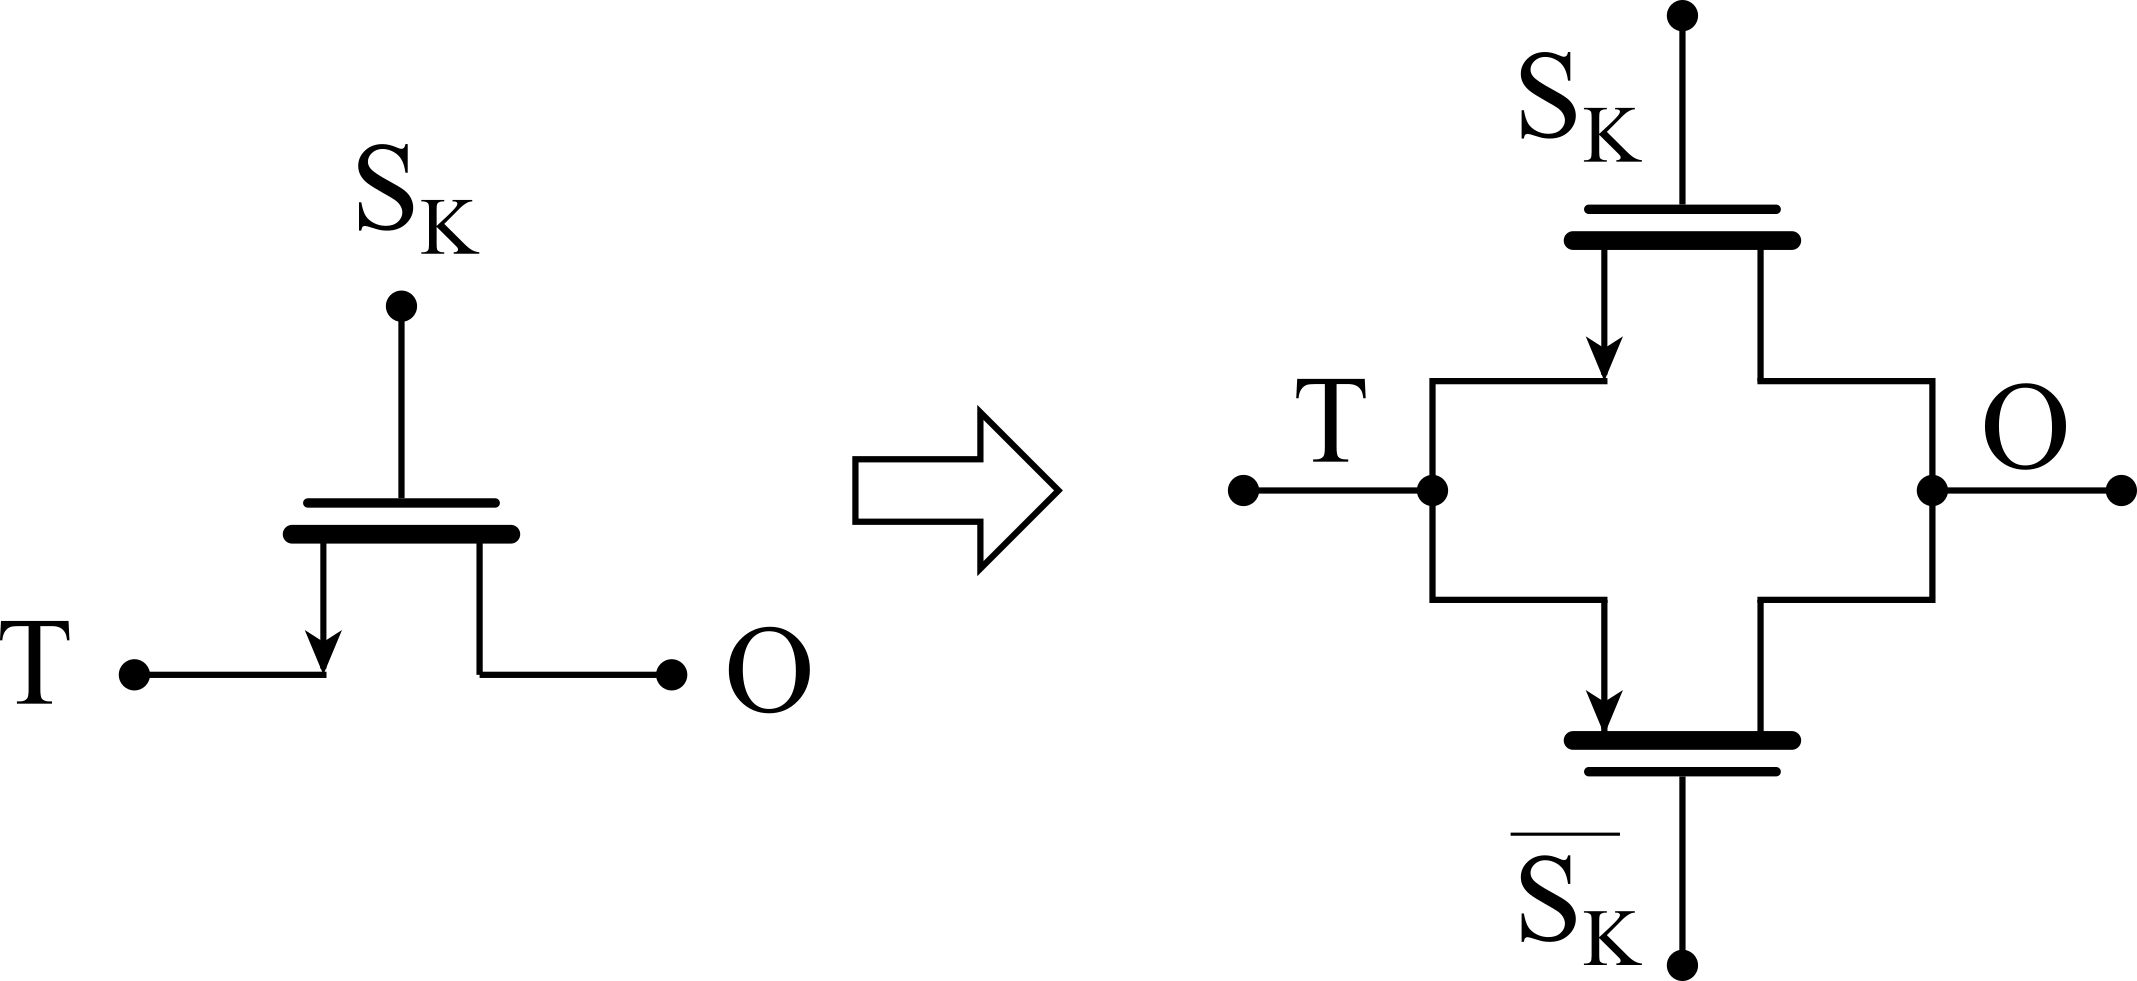
\includegraphics[width=0.5\columnwidth]{Chap05/Figures/transmission_gate.png}
\caption{Transmission Gate}
\label{fig:trans_gate}
\end{figure}
%
Different techniques exists to solve this problem arising from unit element mismatch resulting into the non-linearity. The Dynamic Element Matching (DEM) technique is one of them and it's implementation is done as shown in Fig. \ref{fig:dwa}. It it comprised of switching matrix and the selection logic. Switching matrix is shown just with NMOS switches, just for the representation, however, every switch in the design is consists of a pair of transmission gate switch, as shown in Fig. \ref{fig:trans_gate}. The switching matrix acquires the thermometer code ($T_7$ to $T_1$) from the flash ADC and pass it to the outputs ($O_7$ to $O_1$) with different combination depending upon the state of the selection logic ($S_7$ to $S_1$).
%
\begin{table}[h!]
\centering
\begin{tabular}{c|c|c|c|c|c|c|c|c|c|c|c|c|c}
\Xhline{4\arrayrulewidth}
\textbf{S\textsubscript{7}} & \textbf{S\textsubscript{6}} & \textbf{S\textsubscript{5}} & \textbf{S\textsubscript{4}} & \textbf{S\textsubscript{3}} & \textbf{S\textsubscript{2}} & \textbf{S\textsubscript{1}} & \textbf{O\textsubscript{7}} & \textbf{O\textsubscript{6}} & \textbf{O\textsubscript{5}} & \textbf{O\textsubscript{4}} & \textbf{O\textsubscript{3}} & \textbf{O\textsubscript{2}} & \textbf{O\textsubscript{1}} \\ \hline
1 & 0 & 0 & 0 & 0 & 0 & 0 & T\textsubscript{7} & T\textsubscript{6} & T\textsubscript{5} & T\textsubscript{4} & T\textsubscript{3} & T\textsubscript{2} & T\textsubscript{1} \\ \hline
0 & 1 & 0 & 0 & 0 & 0 & 0 & T\textsubscript{1} & T\textsubscript{7} & T\textsubscript{6} & T\textsubscript{5} & T\textsubscript{4} & T\textsubscript{3} & T\textsubscript{2} \\ \hline
0 & 0 & 1 & 0 & 0 & 0 & 0 & T\textsubscript{2} & T\textsubscript{1} & T\textsubscript{7} & T\textsubscript{6} & T\textsubscript{5} & T\textsubscript{4} & T\textsubscript{3} \\ \hline
0 & 0 & 0 & 1 & 0 & 0 & 0 & T\textsubscript{3} & T\textsubscript{2} & T\textsubscript{1} & T\textsubscript{7} & T\textsubscript{6} & T\textsubscript{5} & T\textsubscript{4} \\ \hline
0 & 0 & 0 & 0 & 1 & 0 & 0 & T\textsubscript{4} & T\textsubscript{3} & T\textsubscript{2} & T\textsubscript{1} & T\textsubscript{7} & T\textsubscript{6} & T\textsubscript{5} \\ \hline
0 & 0 & 0 & 0 & 0 & 1 & 0 & T\textsubscript{5} & T\textsubscript{4} & T\textsubscript{3} & T\textsubscript{2} & T\textsubscript{1} & T\textsubscript{7} & T\textsubscript{6} \\ \hline
0 & 0 & 0 & 0 & 0 & 0 & 1 & T\textsubscript{6} & T\textsubscript{5} & T\textsubscript{4} & T\textsubscript{3} & T\textsubscript{2} & T\textsubscript{1} & T\textsubscript{7} \\ \Xhline{4\arrayrulewidth}
\end{tabular}
\caption{The Output codes of the DEM based on the selection logic}
\label{tab:dem}
\end{table}
%
The Tab. \ref{tab:dem} shows how the flash ADC thermometer code is passed to the output for given combination of selection logic. Extra features are also added to the DEM such as Enabling or disabling of DEM and resetting of the DEM. When DEM is disabled, the selection logic freezes the configuration to the state where $S_7$ is logic high and other selection bit ($S_6$ to $S_1$) are logic low. This feature helps to know the SNDR improvement.


\subsection{Timing Block}
%
\begin{figure}[h!]
\centering
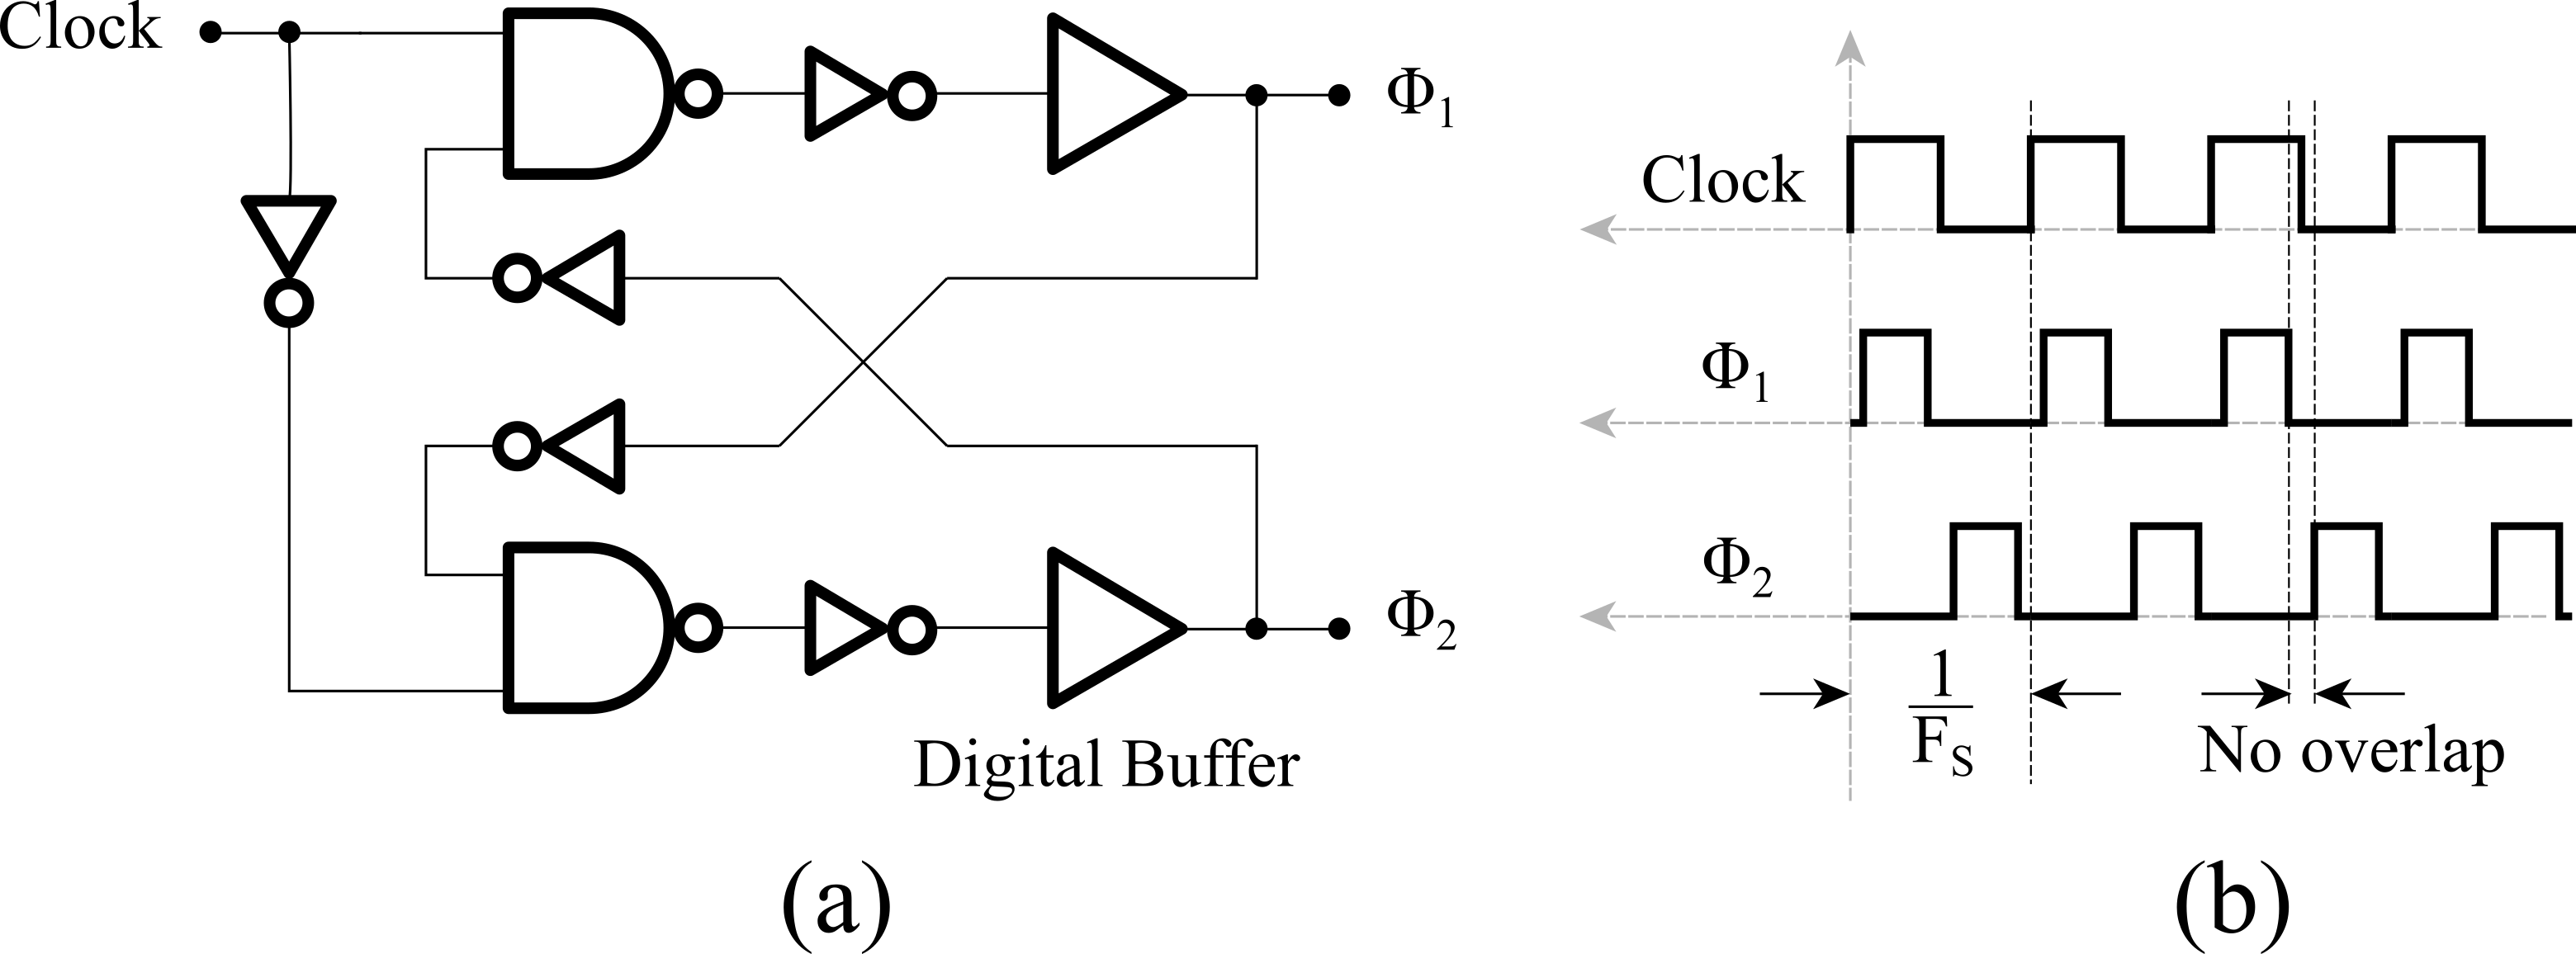
\includegraphics[width=\columnwidth]{Chap05/Figures/timing_circuit_phases.png}
\caption{Schematic for generation of non-overlapping clock phases}
\label{fig:clk_phase_circuit}
\end{figure}
%
The schematic of the non-overlapping phase generator is depicted in Fig. \ref{fig:clk_phase_circuit}. The implementation has been done in order to derive the two non-overlapping clock phases $\Phi_1$ and $\Phi_2$ (and their complements $\overline{\Phi_1}$ and $\overline{\Phi_2}$, not shown in figure). It is also possible, if required, to pull-out the advanced and (or) the delayed versions of these phases through the buffers by revising the locations of the nodes through which the signals has to be pulled out. The non-overlapping time for the designed phase-generator working at 80~MHz is around 1.25~ns. 
%
\begin{figure}[h!]
\centering
\includegraphics[width=\columnwidth]{Chap05/Figures/mod_18_counter.png}
\caption{Schematic for generation of the different control signals for IADC and ISG}
\label{fig:cntrl_sigs}
\end{figure}
%
After the fundamental phases are derived, some special control signals are required by the inter-stage gain (ISG) block such as phases for sampling the residue ($\Phi_{sampl}$), amplifying the residue ($\Phi_{ampl}$) and resetting the ISG ($\Phi_{ISGRST}$) while IADC requires the signals such as $\Phi_{EOC}$ and $\Phi_{RST}$.
These signals are generated by employing MOD-24 counter and a combinational logic as shown in Fig. \ref{fig:cntrl_sigs} and signals are depicted in Fig. \ref{fig:timing_cntrl_sigs}. 
%
\begin{figure}[h!]
\centering
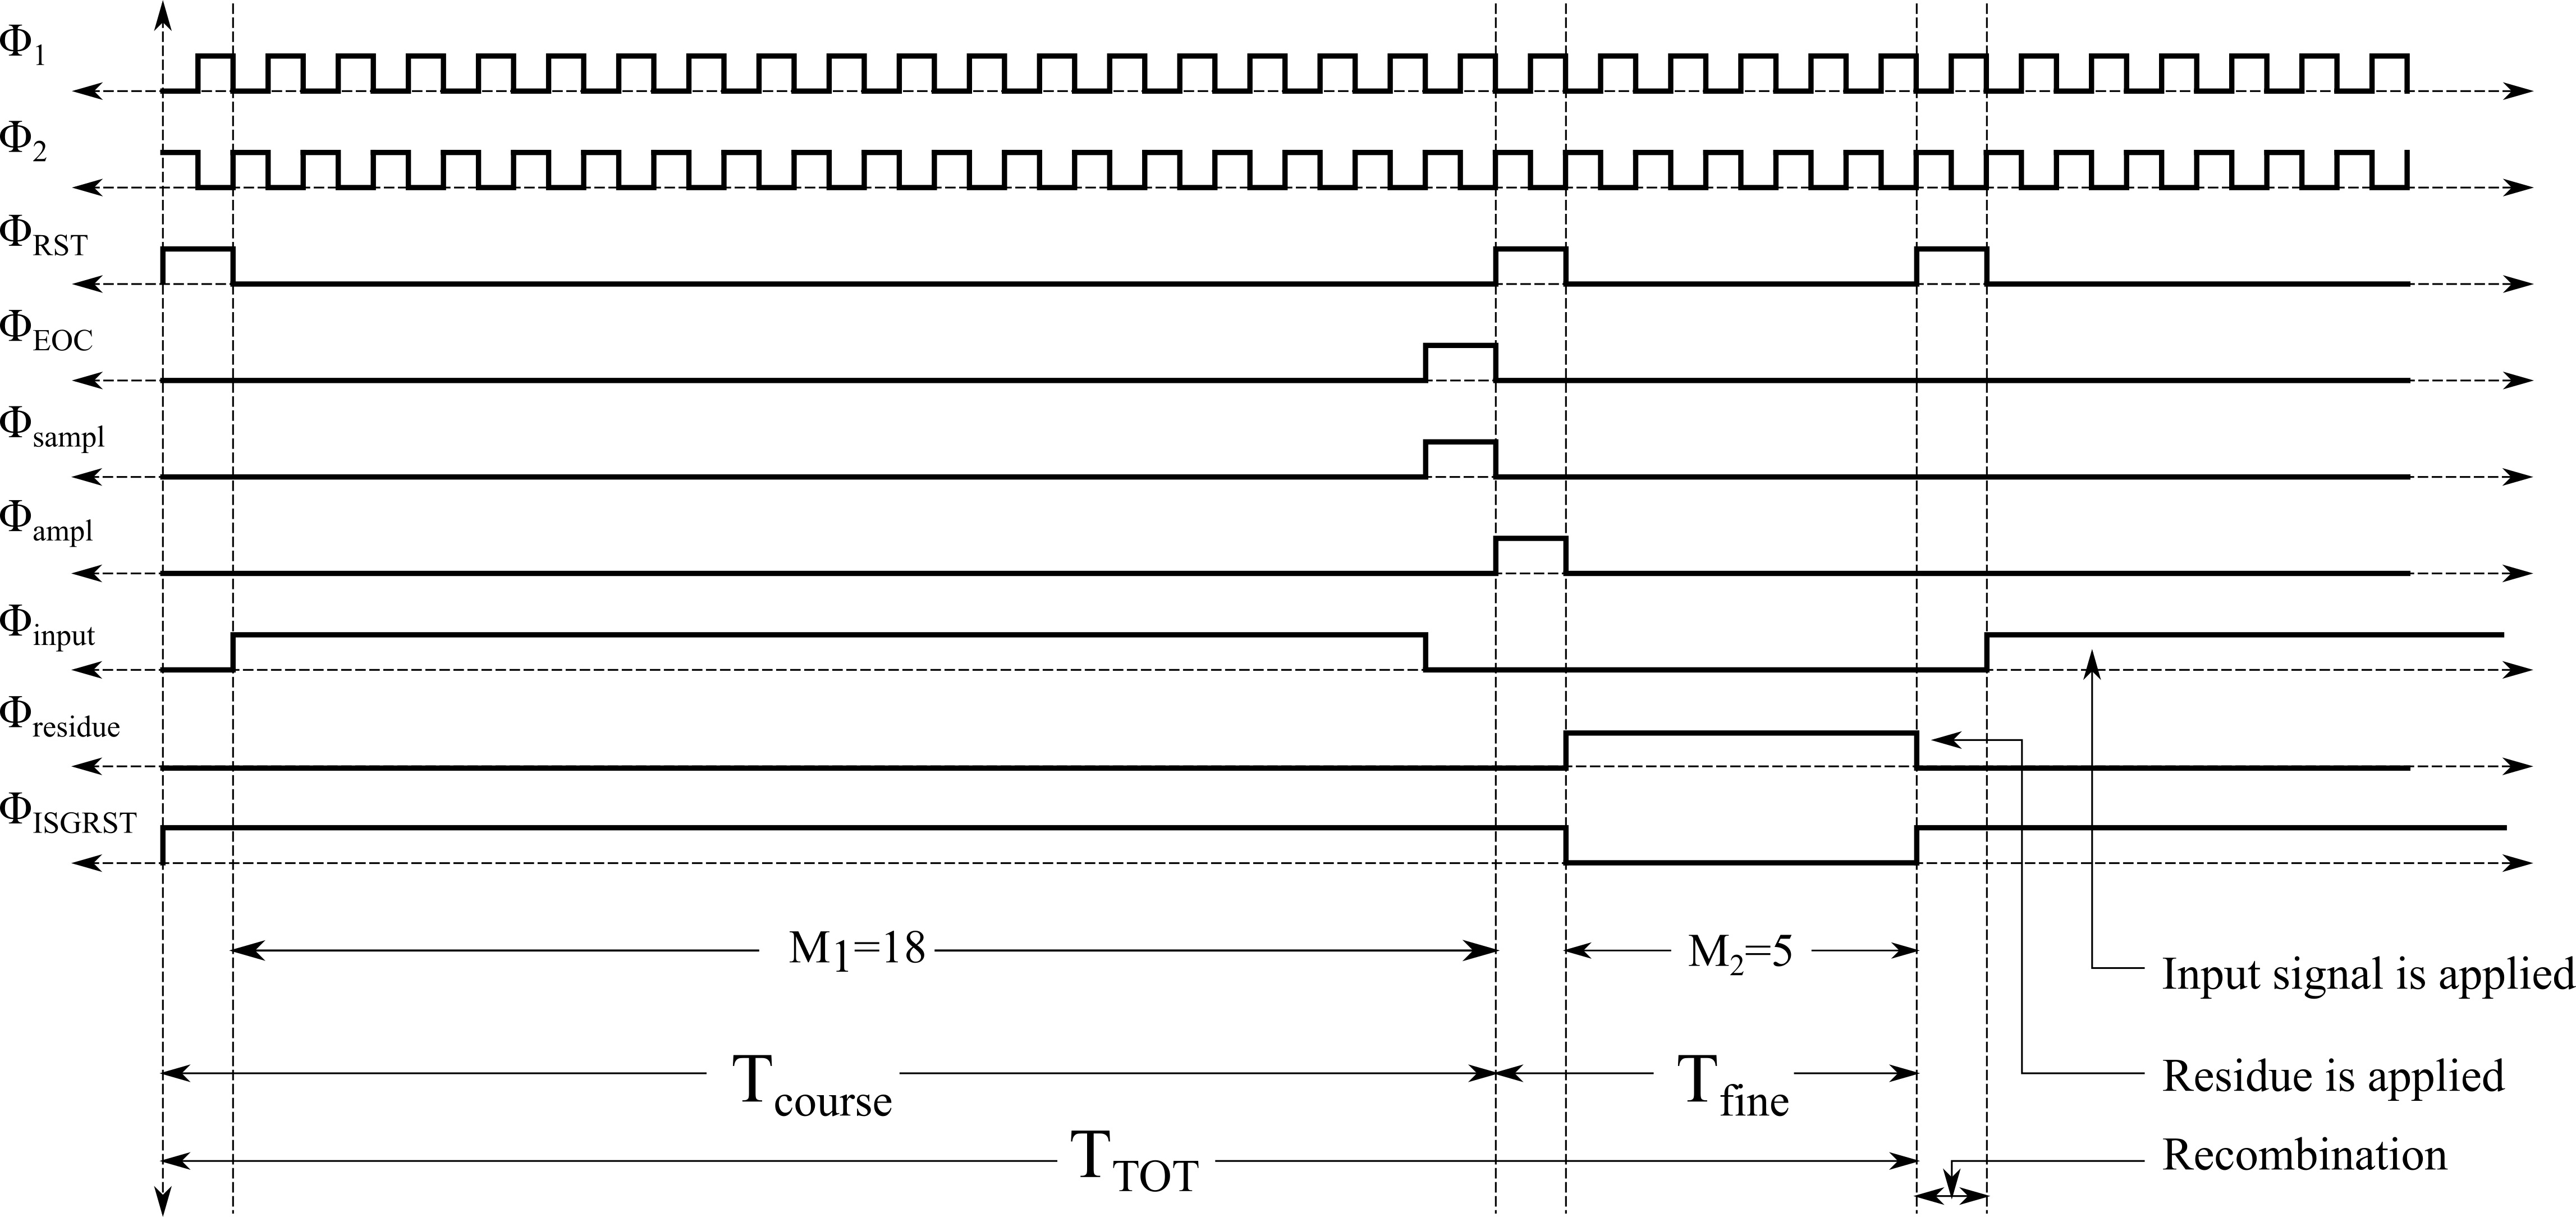
\includegraphics[width=\columnwidth]{Chap05/Figures/timing_control_phases.png}
\caption{Timing diagram of the different control signals for IADC and ISG}
\label{fig:timing_cntrl_sigs}
\end{figure}
%
\subsection{Thermometer to Binary Conversion}
%
\begin{figure}[h!]
\centering
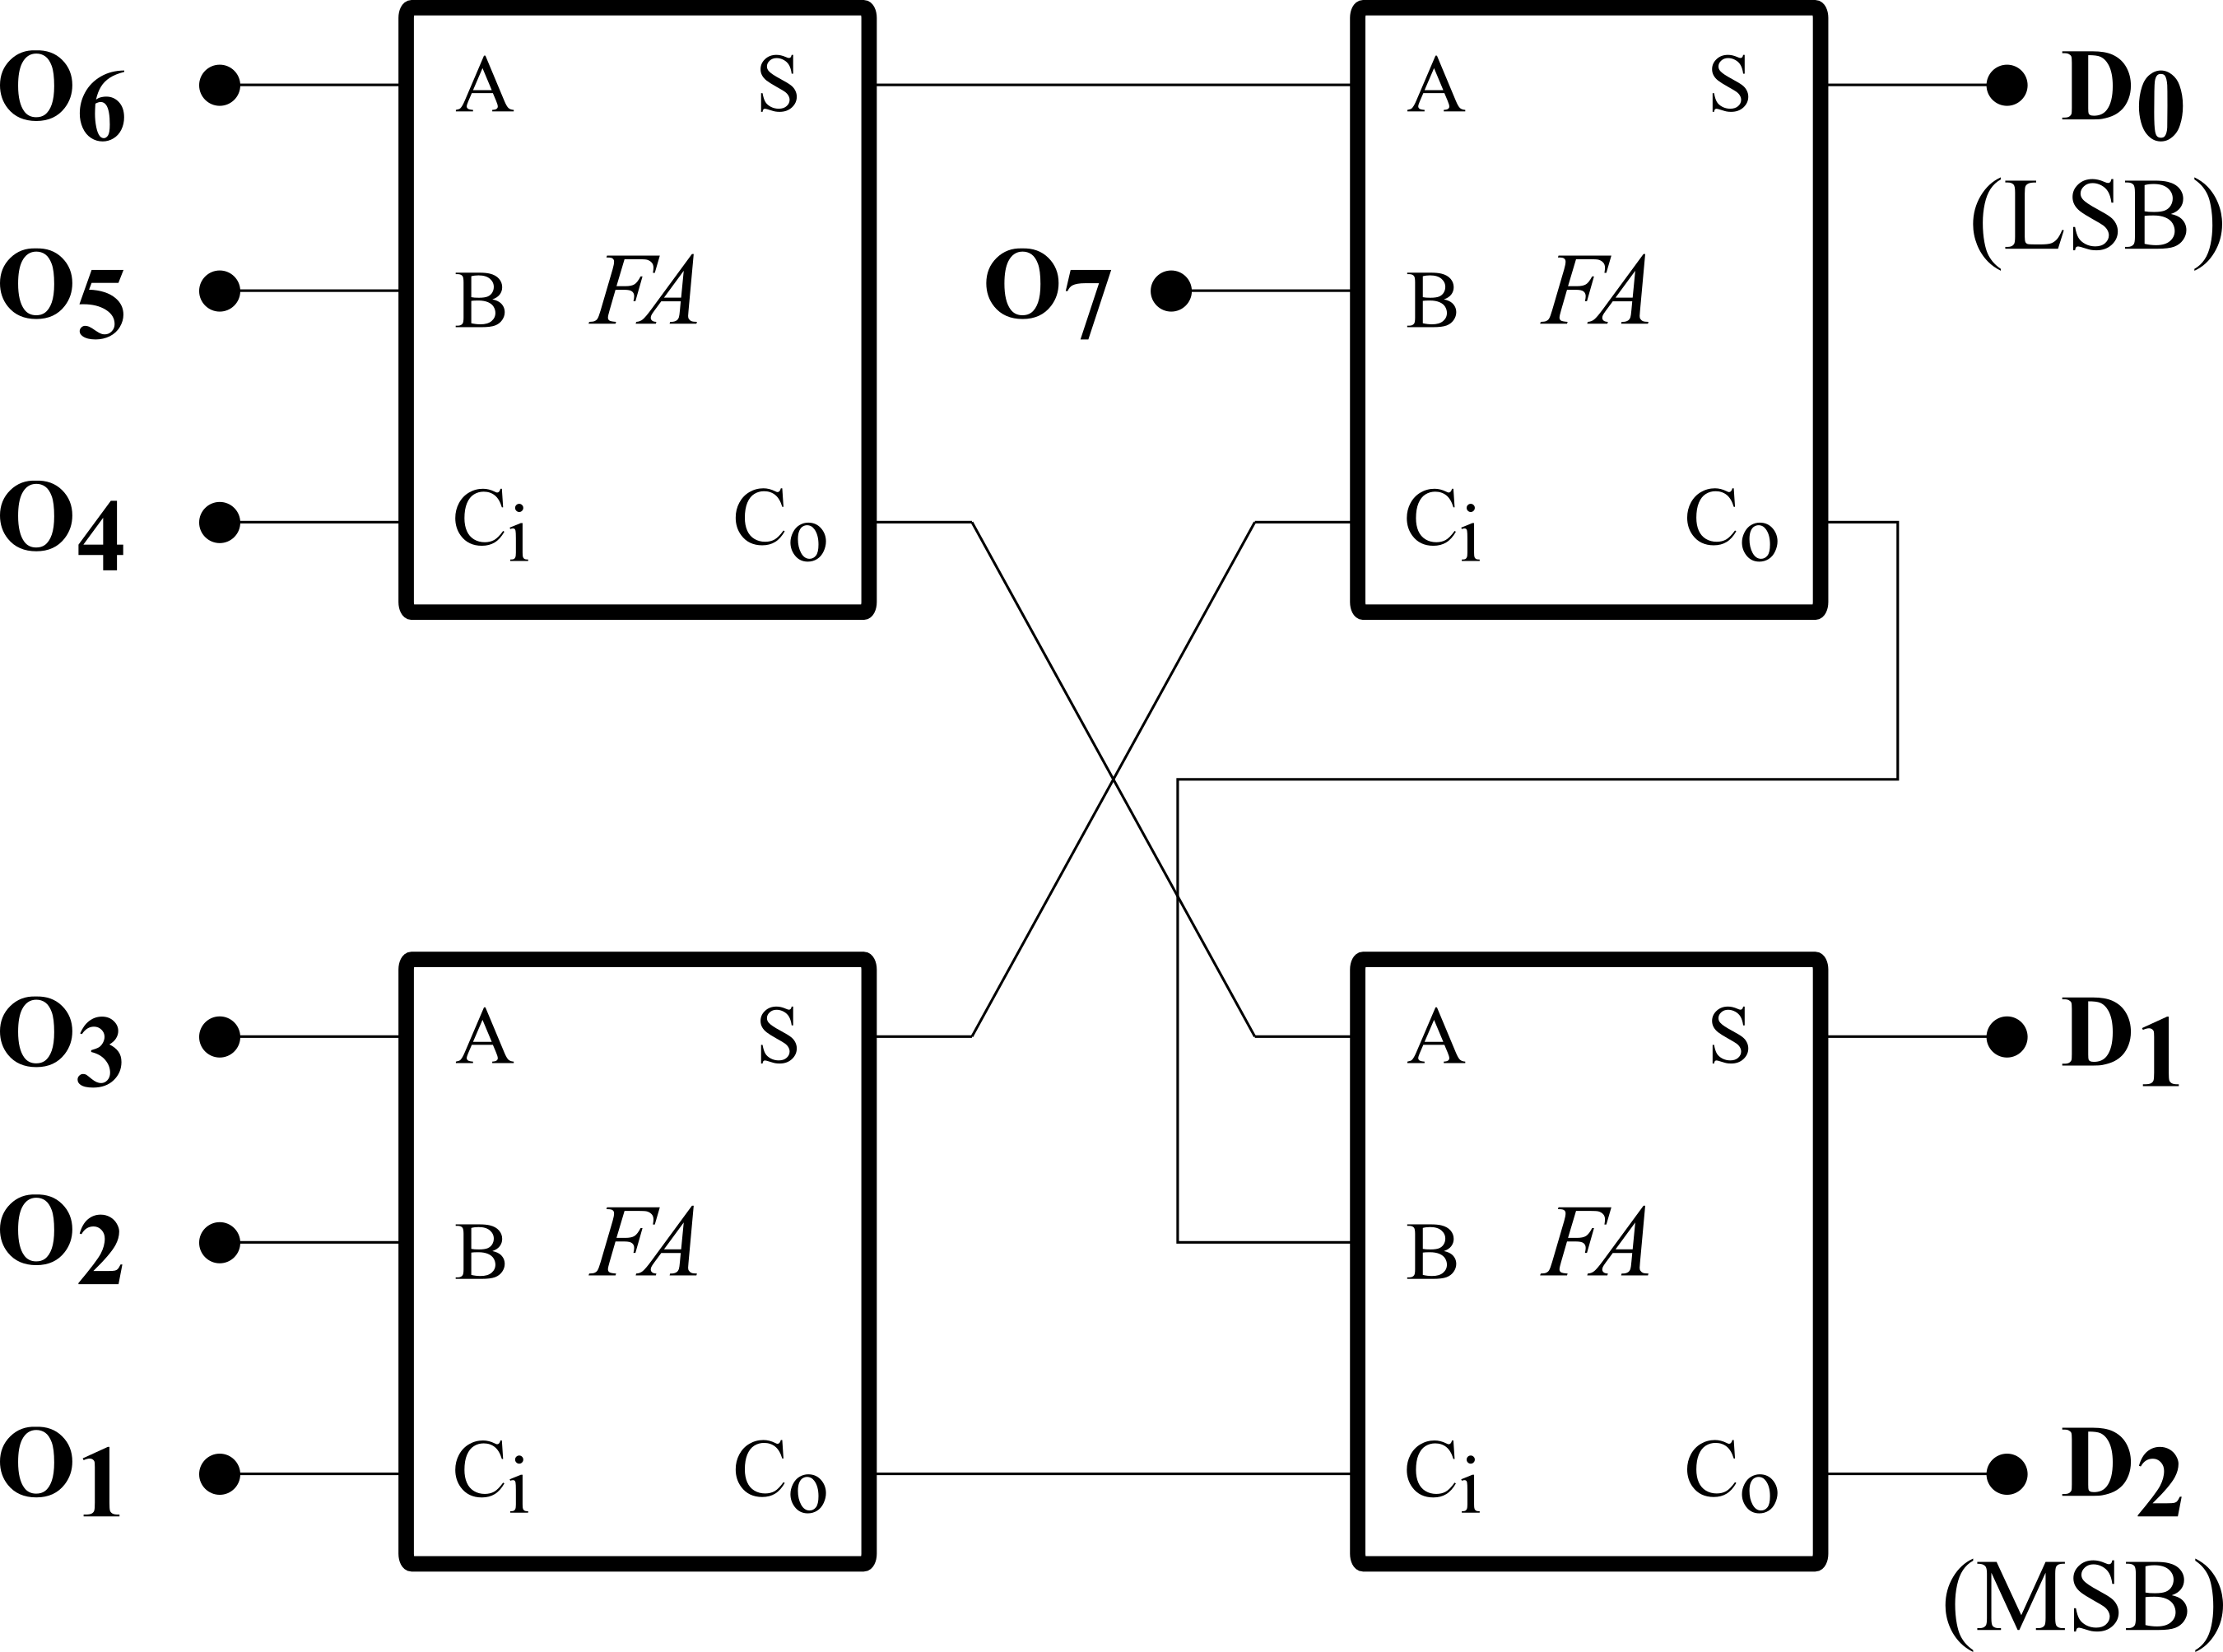
\includegraphics[width=0.5\columnwidth]{Chap05/Figures/wallece_tree.png}
\caption{Thermometer to Binary Encoder}
\label{fig:wallece_tree}
\end{figure}
%
A 7-bit thermometer code delivered by the flash ADC must be converted into a 3-bit binary code so as to ease the interface of the chip to the instrument reading the bit during the measurements. Therefore, a thermometer-to-binary encoder is employed as depicted in Fig. \ref{fig:wallece_tree}. The basic building block of this encoder is a full-adder (FA). The full adder counts the number of ones present at it's input and produces the sum $S$ and carry $C_o$. The encoder is also called as a ones counter since it counts the total number of 1s delivered by flash ADC and converts it into binary code. Even in presence of the bubble, this encoder works efficiently and converts into a correct binary code, this encoder is advantageous. The number of full adder cells needed for implementation of n-bit binary encoder is given as,
%
\begin{equation}
    K_n = \sum^{n}_{i=1}\left(i-1\right)2^{(n-i)}
\end{equation}
%

\begin{figure}[h!]
\centering
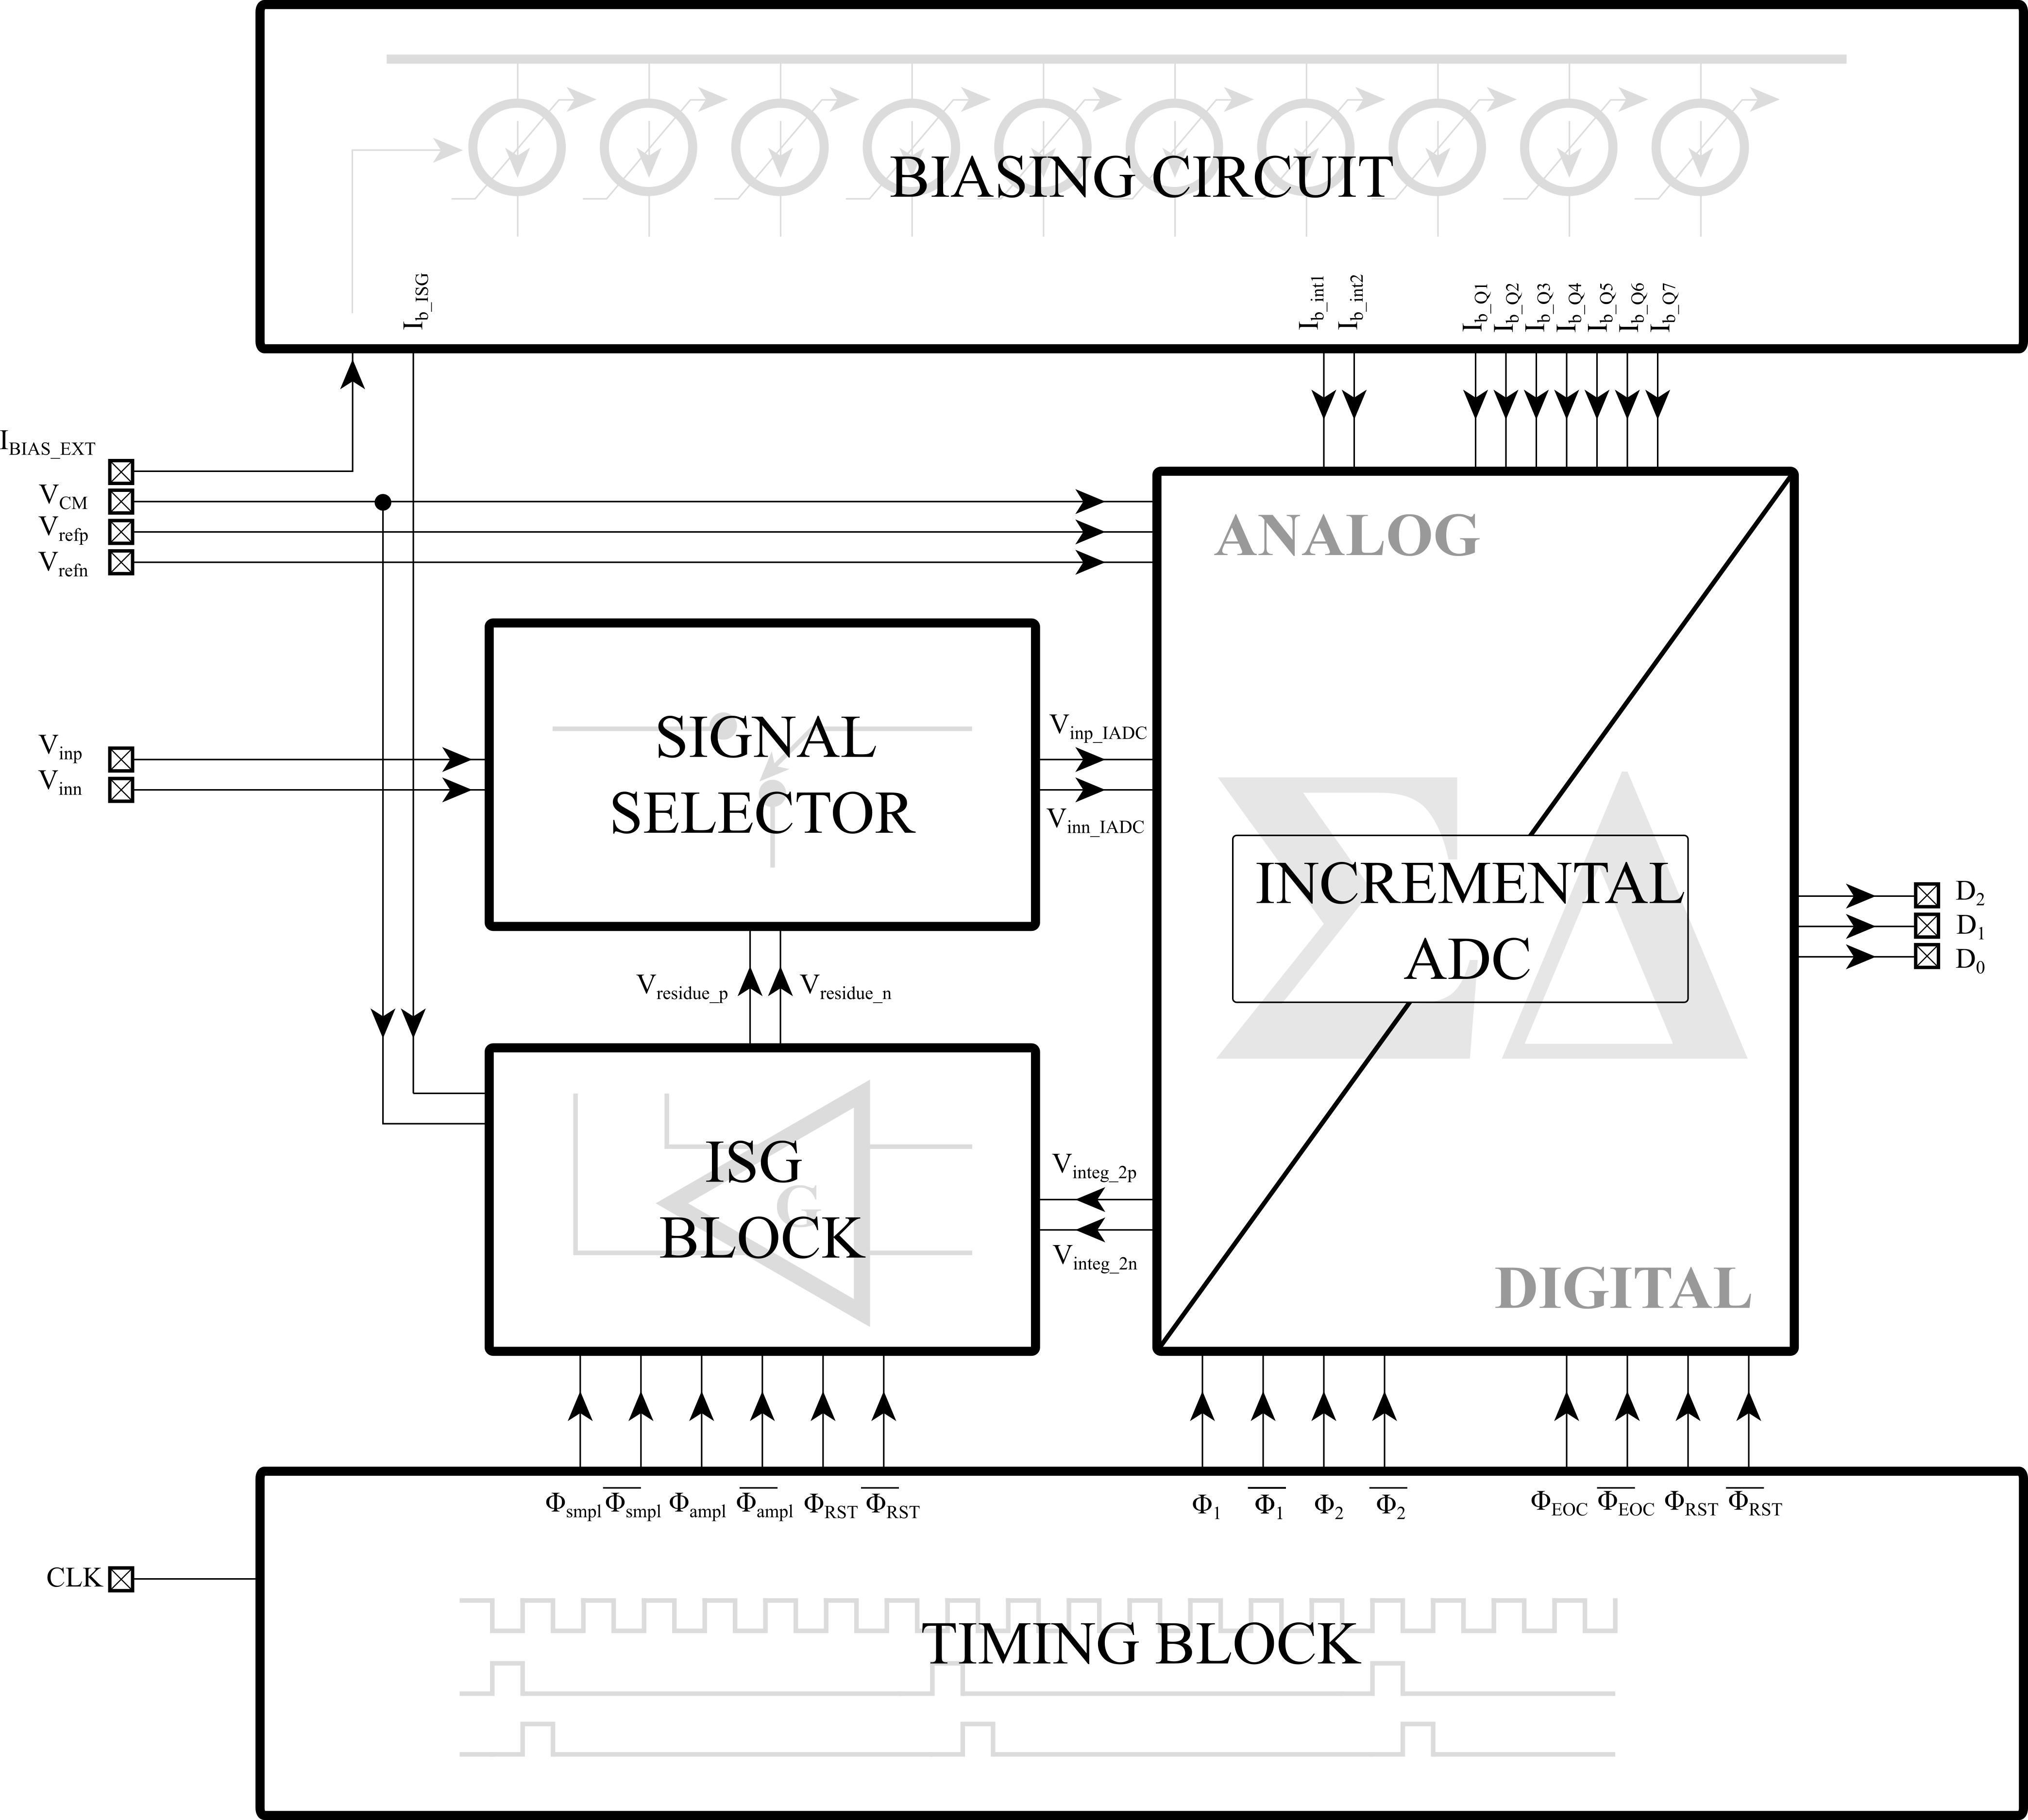
\includegraphics[width=\columnwidth]{Chap05/Figures/block_diagram.png}
\caption{Block Diagram of full architecture of ERADC with core and the supporting blocks}
\label{fig:block_diagram}
\end{figure}